\documentclass{article}
% \usepackage{arxiv}  % arxiv preprint style — replace with JBES template at submission time
\usepackage[margin=1in]{geometry}
\newcommand{\headeright}{}
\newcommand{\undertitle}{}
\newcommand{\shorttitle}[1]{}
\providecommand{\keywords}[1]{\noindent\textbf{Keywords:} #1\par}
\usepackage[utf8]{inputenc}
\usepackage[T1]{fontenc}
\usepackage{hyperref}
\usepackage{url}
\usepackage{booktabs}
\usepackage{amsfonts}
\usepackage{amsmath}
\usepackage{amssymb}
% \usepackage{nicefrac}  % unused
\usepackage{graphicx}
\usepackage{natbib}
\usepackage{doi}
\usepackage{tikz}
\usepackage{pgfplots}
\pgfplotsset{compat=1.18}
\usepgfplotslibrary{fillbetween}
\usetikzlibrary{shapes,arrows,positioning,calc,backgrounds,fit,patterns,decorations.pathreplacing}

% --- Okabe-Ito triplet restricted to our three cities (colorblind-safe, prints in grey)
\definecolor{cBOS}{HTML}{999999}
\definecolor{cNYC}{HTML}{0072B2}
\definecolor{cSF}{HTML}{D55E00}
\definecolor{cMUTE}{HTML}{BBBBBB}
% Okabe-Ito extensions for the 12-city / three-channel v3 figures (colorblind-safe)
\definecolor{cGRN}{HTML}{009E73}
\definecolor{cPNK}{HTML}{CC79A7}
\definecolor{cSKY}{HTML}{56B4E9}
\definecolor{cYEL}{HTML}{E69F00}

% --- Shared axis style (Tufte-aligned)
\pgfplotsset{
  causalre/.style={
    axis lines*=left,
    title style={font=\normalsize},
    label style={font=\small},
    tick label style={font=\scriptsize},
    legend style={font=\scriptsize, draw=none, fill=none, row sep=1pt},
    every axis plot/.append style={thick},
    axis on top,
  },
  causalre body/.style={ causalre, width=0.45\textwidth, height=6cm, },
  causalre wide/.style={ causalre, width=0.7\textwidth, height=0.6\textwidth, },
  causalre strip/.style={ causalre, width=5.0cm, height=4.5cm,
                          title style={font=\small} },
}
\usepackage{amsthm}
\usepackage{algorithm}
\usepackage{algorithmic}
\usepackage{placeins}
\usepackage{float}

% Define theorem environments
\newtheorem{proposition}{Proposition}
\newtheorem{hypothesis}{Hypothesis}
\newtheorem{theorem}{Theorem}
\newtheorem{lemma}{Lemma}
\newtheorem{definition}{Definition}
\newtheorem{corollary}{Corollary}
\newtheorem{assumption}{Assumption}
\newtheorem{remark}{Remark}

\title{Causal Disentanglement of Location and Semantic Signals in Real Estate Valuation}

\author{
    Brandon Yee$^{1,*}$ \quad Jacob Crainic$^{1,*}$\\
    $^{1}$Management Sciences Lab, Yee Collins Research Group\\
    \texttt{\{b.yee, j.crainic\}@ycrg-labs.org}\\
    $^{*}$Equal contribution; co-first authors.
}

{\tiny \date{}}

\renewcommand{\headeright}{Preprint}
\renewcommand{\undertitle}{Preprint}
\renewcommand{\shorttitle}{Causal Disentanglement in Real Estate Valuation}

\begin{document}
\maketitle

\begin{abstract}
Automated valuation models increasingly read the prose of a property listing
alongside its structured attributes, and the language reliably sharpens their
price predictions, yet a gain in predictive accuracy cannot by itself reveal
whether the text contributes genuine information about a property or merely
relabels the neighborhood geography that an agent's description inevitably
carries. We take that ambiguity as the object of study, treating the leading
direction of a listing embedding as a high-dimensional treatment whose effect on
log sale price we estimate with a partially linear double machine learning score,
and we ask how much of that effect survives once location is taken out of the
picture. The question is one of spatial confounding, the familiar difficulty in
which an exposure and an unmeasured driver of the outcome share a geographic
pattern, and the apparatus we assemble around it pairs cross-fitted
gradient-boosted nuisances with a closed-form concept-erasure projector that
strips latitude and longitude from the representation, a fixed-treatment toggle
that adds a flexible location basis to the controls, an intervention that rewrites
listings with a large language model, and a finite-sample calibration study.
What that apparatus turns up is more reassuring than the predictive-fit worry
would lead one to expect. The embedding does encode location, recoverable by a
held-out probe at an $R^2$ reaching one half before erasure and essentially
nothing after, and even so, holding the text treatment fixed while adjusting for
geography leaves its per-standard-deviation price effect almost unmoved across
eleven of twelve metropolitan markets, so that what the language contributes is in
most places semantic content rather than geography in disguise. The surviving
signal proves robust to the choice of encoder, with a Doc2Vec uniqueness measure
and a sentence-BERT principal component tracking one another closely from market
to market, while remaining strongly heterogeneous in magnitude and showing its
one clear spatial exception in New York, the market whose own text direction is
the most geographic of the twelve. Because the estimates are associational rather
than cleanly identified, we bound their fragility with a sensitivity analysis that
fixes how weak an unobserved confounder would have to be to overturn each market's
result, and we document in passing that the influence-function interval double
machine learning reports for an embedding-valued treatment undercovers at the
sample sizes a single market affords, for which a bootstrap over the full pipeline
is the remedy. The contribution is accordingly a disciplined protocol for
measuring and deconfounding the price effect of a learned text representation,
together with the inferential caution that protocol demands, rather than a causal
elasticity of price on language.
\end{abstract}

\keywords{Spatial Confounding \and Concept Erasure \and Double Machine Learning \and Generated Regressors \and Text as Data \and Real Estate Valuation}

\section{Introduction}

Automated valuation models increasingly read the natural-language description of a property alongside its structured attributes, and the text reliably improves their predictions, with \citet{shen2021information}, \citet{baur2023automated}, and \citet{lorenz2023interpretable} all reporting sizable reductions in pricing error once listing-text embeddings are added on top of location and the usual structured controls. The reading almost always attached to that improvement is the optimistic one, that listing language carries information about a property which its tabular attributes miss, and on its face the reading is plausible, because a good description does say things about condition, light, and finish that no bedroom count records. What predictive accuracy cannot do, however, is tell that interpretation apart from a more deflationary one, since property descriptions are written by agents who know exactly where a listing sits, so any embedding of those descriptions absorbs the neighbourhood whether the encoder intends it to or not, and a model that prices the embedding may be doing little more than relabelling location as semantic content. Because the two stories make identical predictions, the very gain that motivates text-augmented valuation is by construction silent on whether the language adds anything at all once geography is accounted for, and it is that silence the paper sets out to break.

Breaking that silence means treating the listing embedding as a high-dimensional treatment and asking how much of its association with sale price is owed to geography rather than to anything the language contributes on its own. The question is an instance of spatial confounding, the difficulty in spatial statistics in which an exposure of interest and an unmeasured confounder share a geographic pattern, so that ordinary regression hands the confounder's effect to the exposure~\citep{paciorek2010importance,hodges2010spatial}, and the discipline's usual remedy, restricting the exposure to the orthogonal complement of the spatial effect~\citep{reich2021spatial,dupont2022spatial}, has a natural counterpart once the exposure is a learned representation. Whether the representation carries location at all is something we can read off directly, by applying the closed-form concept-erasure projector of \citet{belrose2023leace}, with an iterative nonlinear pass~\citep{iskander2023shielded} for the leakage a linear projector leaves behind, and asking how well a held-out probe can still recover the coordinate from what survives. The separate and more consequential question of whether that location actually drives the price effect calls for a separate instrument, and we answer it by holding the text treatment fixed inside a partially linear Double Machine Learning score~\citep{robinson1988root,chernozhukov2018double} while moving geography on and off the confounder side, the contrast that a Gelbach decomposition makes precise. Running the framework without exclusion across twelve metropolitan markets then lets the answer be read as a distribution rather than a single number, since the embedding geometry, the structured covariates, and the listing density that decide how much room the text has once location is accounted for all differ from one market to the next.

The deconfounding test that this design supports returns an answer more reassuring than the predictive-fit worry would suggest, and the route it takes to that answer is worth following carefully, because the most obvious reading of the erasure diagnostic seems at first to point the other way. A held-out probe recovers the latitude-longitude coordinate from the embedding at an $R^2$ that climbs toward one half, so the representation unmistakably carries location, and the natural expectation is that the price effect of its leading direction would dissolve once that geography were taken out, and yet that is not what happens, because holding the text direction fixed as the treatment and folding a flexible location basis into the controls leaves its per-standard-deviation effect on log price almost exactly where it began across eleven of the twelve markets, while the single market in which the adjustment does bite, New York, turns out to be the one whose text direction is itself the most geographic, so that the exception illuminates the mechanism rather than embarrassing it. What the design settles about the magnitude of the effect is matched by what it forces us to confront about the standard error, since the leading principal component is estimated on the very sample that estimates the price effect and therefore behaves as a generated regressor in the sense of \citet{pagan1984econometric}, the orthogonal-score variance of \citet{chernozhukov2018double} does not absorb the extra sampling variability this introduces, and the analytic interval comes out anticonservative at the few thousand listings a single metropolitan market affords, a shortfall we document in a calibration study and repair with a bootstrap that resamples the entire pipeline. Beneath the generated-regressor problem sits the eigengap of the embedding covariance, and a sin-$\Theta$ stability argument ties how faithfully the estimated treatment direction tracks its population target to the size of that gap, which is finally what licenses treating the leading component as a stable object to put on the left of a causal question.

Applied across twelve metropolitan areas using $3{,}851$ deduplicated Redfin listings, the framework returns a picture whose parts hang together. Listing text carries a positive per-standard-deviation association with log sale price that holds up regardless of which encoder produces it, since a Doc2Vec uniqueness channel and a sentence-BERT principal component move almost in lockstep from market to market and so read as two encodings of a single signal rather than as independent confirmations of it. That association varies strongly in magnitude across the twelve markets, it survives the spatial deconfounding just described everywhere but New York, and it is not organised by any metropolitan demographic moderator that withstands multiplicity adjustment and leave-one-out leverage diagnostics on so few units. None of this amounts to a clean causal elasticity, and we are careful to say so throughout, because the estimates remain associational rather than identified by design, and the sensitivity analysis we run in the style of \citet{cinelli2020making} fixes how weak an unmeasured confounder would have to be to overturn each market's result, a threshold that comes out uncomfortably modest in several of them. What the paper offers in the end is a disciplined protocol for measuring and deconfounding the price effect of a learned text representation, carried out with inference calibrated to the embedding-treatment setting, and we release the data and the code so that the protocol can be reused rather than only read.

We have arranged what follows in the order a skeptical reader would want to work through it. The literatures on spatial confounding, on concept erasure, and on text as a treatment have grown up largely apart from one another, and Section~\ref{sec:related} brings them into contact, after which the estimand and the linear and nonlinear erasure pipeline on which the later analysis leans are developed in Section~\ref{sec:methods}. How the corpus was assembled, and audited for the duplication that scraped listings invite, is the business of Section~\ref{sec:data}, and the calibration study behind our inferential caution is documented in Appendix~\ref{app:simulation}, where the influence-function interval is shown to undercover for an embedding treatment and an out-of-fold construction of the treatment direction restores most of the lost coverage. The twelve-market evidence occupies Section~\ref{sec:results}, which moves in turn through the uniqueness and principal-component estimates, the rewriting intervention, the erasure and decomposition diagnostics, the sensitivity bounds, and the cross-method comparison, before Section~\ref{sec:conclusion} closes by drawing the line, for practice, between what a predictive-only evaluation of text-augmented valuation can and cannot support.

\section{Related Work}
\label{sec:related}

\subsection{Listing text in automated valuation, and the question it raises}
\label{sec:related_disparities}

The use of natural language in property valuation predates the recent enthusiasm for embeddings, and the empirical claim that listing text improves prediction is by now well established. \citet{nowak2017textual} show that the free-text remarks attached to a multiple-listing record reduce pricing error substantially once they are encoded, and \citet{nowak2021dictionaries} document that the vocabulary doing the predicting shifts from one submarket to the next. A particular channel is formalised by \citet{shen2021information}, who measure the textual uniqueness of a description relative to its neighbours and report a uniqueness premium on the order of ten to fifteen percent per standard deviation in a single metropolitan market, while \citet{baur2023automated} show that folding a sentence-embedding representation into a structured valuation model lowers its error by as much as a sixth. With few exceptions the literature reads gains of this kind as evidence that language carries information about a property which its tabular attributes do not.

What that reading passes over is that an agent writes a description already knowing exactly where the property sits, so the language is saturated with location before any encoder touches it, and a representation learned from such text will carry the neighbourhood whether or not it carries anything more. Because a predictive metric cannot tell a model that prices genuine semantic content apart from one that prices laundered geography, the very gains that motivate text-augmented valuation are silent on which of the two is operating, and the question of how much of the apparent text effect is real has gone largely untested in a causal register even as the predictive work has matured. We take up that question directly, and the apparatus it calls for sits at the meeting point of three literatures that have seldom been brought into the same room, namely the treatment of text as a causal variable, the spatial-statistics account of confounding by location, and the concept-erasure methods developed in natural language processing for removing a named attribute from a representation. The same machinery bears on the fairness and auditability concerns that motivate much of the recent scrutiny of automated valuation, since \citet{neal2024racial} and \citet{wang2025racial} document residual valuation gaps that survive architectural improvement and a text feature re-encoding neighbourhood geography re-encodes whatever that geography is correlated with, but the object of this paper is the prior measurement question of whether the text effect is genuine at all rather than the disparities a confirmed effect would carry.

\subsection{From Hedonic Models to Multimodal Valuation}

The idea that property values can be decomposed into contributions from observable characteristics dates to the hedonic pricing framework~\citep{rosen1974hedonic,sheppard1999hedonic}. Automated valuation models built on this foundation through progressively richer statistical machinery: generalized additive models~\citep{gloudemans1999mass}, spatial autoregressive specifications that account for price correlation among neighboring properties~\citep{pace1998sparse,can1992specification}, and kriging-based approaches that interpolate unobserved spatial surfaces~\citep{bourassa2010predicting}. Each generation recognized more clearly that spatial dependence is not a nuisance to be corrected but a first-order feature of housing markets.

Machine learning accelerated this trajectory. Ensemble methods outperform linear hedonic models by capturing non-linear feature interactions automatically~\citep{park2015using,antipov2012mass}, and deep learning extended the input space beyond tabular features to images~\citep{poursaeed2018vision,law2019understanding,you2017building} and text~\citep{shen2021information,baur2023automated}. Visual models trained on property photographs or street-view imagery can estimate luxury level and architectural style~\citep{poursaeed2018vision,lindenthal2021architectural}, while textual models extract semantic features from listing descriptions that correlate with sale prices~\citep{nowak2017textual,law2019house}. Multimodal systems fuse these modalities together, reporting performance gains attributed to complementary information~\citep{bin2020multisource,kang2021human,kostic2020imagefeatures}. Graph neural networks push the idea further by propagating information between spatially proximate properties, so that each node's representation absorbs its neighbors' features~\citep{das2021boosting,lin2021spatial,peng2022lifelong,li2018diffusion,huang2018deepcrime}.

A persistent concern runs through this literature, raised early but seldom addressed. The most predictive words in property descriptions vary across geographic submarkets~\citep{nowak2017textual,nowak2021dictionaries}, visual features capture neighborhood-level rather than property-level variation~\citep{law2019understanding}, architectural style clusters geographically~\citep{lindenthal2021architectural}, and GNN message passing, by design, propagates whatever signal is shared among neighbors, including location-induced price similarity. If text, images, and graph features all encode geography, then fusing them creates the appearance of complementary signal from what is really redundant spatial encoding through different channels.

\subsection{The Semantic Interpretation and Its Limits}

The commercial and research appeal of text-based valuation rests on a specific claim: that property descriptions carry information about value that structured features miss. A one-standard-deviation increase in textual ``uniqueness'' is reported to raise predicted price by 10--15\%~\citep{shen2021information}. Including text embeddings is reported to reduce valuation error by up to 17\%~\citep{baur2023automated}. Hierarchical graph representations that embed similar-value properties near one another in latent space appear to learn price-relevant structure~\citep{zhang2021mugrep}. UMAP projections of these embeddings produce visually appealing clusters that seem to correspond to market segments~\citep{baur2023automated}.

Every one of these findings is also predicted by a model in which text carries zero independent information. If agents in affluent neighborhoods write ``luxury finishes'' and ``steps from fine dining'' while agents in family-oriented suburbs write ``great school district'' and ``quiet cul-de-sac,'' the embeddings will cluster by price segment, SHAP will rank descriptive terms as important~\citep{lorenz2023interpretable,stang2023location}, and adding text to a location-only model will improve $R^2$, even though the entire gain comes from spatially confounded language rather than property-specific content. The assumption that generic quality terms like ``spacious'' or ``renovated'' provide location-independent signal~\citep{lorenz2023interpretable} ignores that ``spacious'' is more frequent in suburban markets and ``renovated'' more frequent in gentrifying urban neighborhoods. \citet{nowak2021dictionaries} find exactly this: the predictive vocabulary shifts across submarkets, suggesting that language mirrors geography rather than transcending it. \citet{wan2023testing} raise the same concern for visual features, proposing system-level tests to determine whether models respond to building attributes or to irrelevant context.

The distinction between correlation and causation is not academic here. If text embeddings genuinely encode value-relevant property attributes independent of location, then NLP-enhanced valuation models offer real information gains. If they primarily encode geography through linguistic patterns, then these models are opaque spatial models and their accuracy gains are expected, not evidence of new signal. Yet across the studies reviewed above, none tests the causal claim. The tools to do so exist in causal inference and spatial statistics, and the confounding structure is transparent, but the question has not been asked. This paper asks it.

\subsection{Spatial Confounding and Attribute Leakage in Learned Representations}

The concern that text may encode geography rather than semantics connects two literatures that have developed largely in parallel.

In spatial statistics and epidemiology, the problem is well characterized: when an exposure of interest varies spatially and shares its spatial pattern with unmeasured confounders, standard regression attributes the confounders' effects to the exposure~\citep{paciorek2010importance}. The severity depends on the spatial scale: fine-grained exposures are most vulnerable to fine-grained confounders. Methods to address this include restricted spatial regression, which orthogonalizes spatial random effects against fixed effects of interest~\citep{reich2021spatial}, and sensitivity frameworks that quantify the confounder strength needed to overturn a finding~\citep{cinelli2020making}. A counterintuitive result from this literature is that adding spatially-correlated error terms to a model can worsen, not improve, inference about fixed effects when spatial confounding is present~\citep{hodges2010spatial}. Spatial econometrics addresses the same challenge through spatial lag and error models~\citep{anselin1988spatial,lesage2009introduction,elhorst2014spatial}, though identification of spatial dependence parameters remains difficult to separate from omitted-variable bias~\citep{gibbons2014spatial}.

In NLP, a parallel line of work has shown that text embeddings absorb far more than semantic content from their training corpora. Word embeddings encode human-like gender and racial biases~\citep{bolukbasi2016man}, replicate implicit association test results~\citep{caliskan2017semantics}, and retain these biases even after standard debiasing~\citep{gonen2019lipstick}. Language use varies systematically by geography: user location can be predicted from tweets with high accuracy~\citep{rahimi2018geolocation}, and lexical innovations diffuse through social networks along spatial paths~\citep{eisenstein2014diffusion}. Property descriptions are an extreme case of this phenomenon because agents write with complete knowledge of the property's location, neighborhood, and market context. The language is not incidentally spatial; it is intentionally so.

Machine learning has begun to develop tools for this class of problem. Causal representation learning seeks representations that reflect causal structure rather than spurious correlation~\citep{scholkopf2021toward,peters2017elements}. Counterfactual fairness formalizes the requirement that predictions be invariant to interventions on protected attributes~\citep{kusner2017counterfactual,kilbertus2017avoiding}. Domain-adversarial networks learn confounder-invariant representations through gradient reversal~\citep{ganin2016domain}, and variational approaches attempt to disentangle causal from spurious factors~\citep{louizos2017causal,moyer2018invariant}. The invariance of causal mechanisms across environments, in contrast to the instability of correlations, motivates transfer-based identification~\citep{rojas2018invariant}. Causal discovery algorithms infer graph structure from data using conditional independence tests~\citep{spirtes2000causation}, score-based search~\citep{chickering2002optimal}, or functional asymmetries between causal directions~\citep{shimizu2006linear,peters2016causal}. Double Machine Learning~\citep{chernozhukov2018double} provides a semiparametric framework for estimating causal effects with machine-learned nuisance parameters at $\sqrt{n}$ rates.

These threads meet in the setting we study, and they have begun to meet elsewhere as well, which is worth stating precisely so that what is new here is not overstated. The idea of adapting a text representation for causal rather than predictive ends is developed by \citet{veitch2020adapting}, whose embeddings are built to retain the confounding-relevant subspace, and the inverse operation of stripping a concept from a document embedding by linear erasure is carried out for similarity and clustering by \citet{fan2025medium}, while \citet{feldman2026causal} treat latent textual features as a treatment whose covariate content has to be residualised away. What this paper adds is therefore neither the erasure operator nor the recognition that a text feature can conflate treatment with confounder, both of which are by now established, but the application of that apparatus to an economic estimand, the price effect of a listing's language, carried out with a design that separates the geography a representation merely encodes from the geography that actually moves the outcome and with inference suited to an embedding-valued treatment. Property valuation is an unusually clean place to attempt this, since location drives both the text and the price, the outcome is measured precisely, and the practical stakes are immediate, and we run the analysis across twelve metropolitan markets rather than the single market the hedonic-text literature has usually examined, which lets the answer be read as a distribution and lets the one market where location does bite be identified rather than assumed away.

\section{Methodology}
\label{sec:methods}

\subsection{Problem Formulation}

Let $\mathcal{D} = \{(x_i, t_i, \ell_i, y_i)\}_{i=1}^n$ denote a dataset of $n$ properties. The variable $x_i \in \mathbb{R}^d$ represents structured property features such as bedrooms, square footage, and age. The variable $t_i \in \mathbb{R}^p$ denotes a text embedding derived from the property description. Geographic location is specified by $\ell_i \in \mathbb{R}^2$ as latitude and longitude coordinates. Finally, $y_i \in \mathbb{R}^+$ represents the sale price or assessed value.

A standard predictive model takes the form $\hat{y}_i = f(x_i, t_i, \ell_i; \theta)$ where $f$ is a learned function parameterized by $\theta$. Recent work reports strong correlations between $t_i$ and $y_i$, interpreting this as evidence that semantic content causally influences property value. However, correlation does not imply causation. Our central objective is to estimate the causal effect of semantic content $t$ on property value $y$, independent of location $\ell$.

\subsection{Structural Causal Model}

We propose the following structural causal model to represent the data-generating process.

\begin{definition}[Real Estate SCM]
The causal relationships among variables are governed by the following structural equations:
\begin{align}
\ell &= U_\ell \label{eq:scm1}\\
x &= f_x(\ell, U_x) \label{eq:scm2}\\
c &= f_c(\ell, U_c) \label{eq:scm3}\\
t &= f_t(\ell, x, c, U_t) \label{eq:scm4}\\
y &= f_y(\ell, x, c, U_y) \label{eq:scm5}
\end{align}
where $U_\ell, U_x, U_c, U_t, U_y$ are mutually independent exogenous variables, and $c$ represents contextual features such as demographics, amenities, and crime statistics.
\end{definition}

The corresponding causal directed acyclic graph is shown in Figure~\ref{fig:dag}.

\begin{figure}[!htbp]
\centering
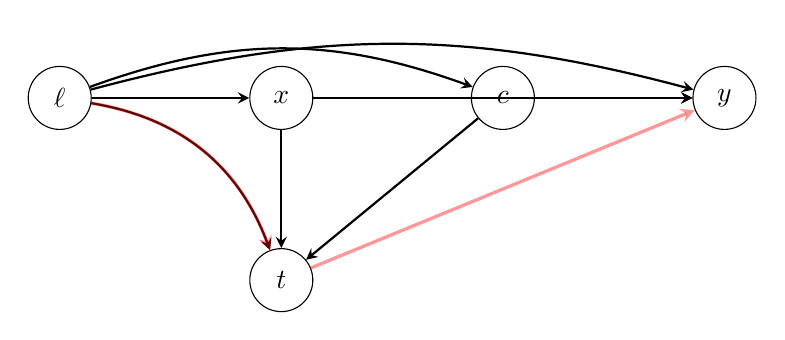
\begin{tikzpicture}[
    node distance=1.5cm and 2cm,
    every node/.style={draw, circle, minimum size=0.8cm},
    arrow/.style={->, >=stealth, thick}
]
    \node (L) {$\ell$};
    \node[right=of L] (X) {$x$};
    \node[right=of X] (C) {$c$};
    \node[below=of X] (T) {$t$};
    \node[right=of C] (Y) {$y$};
    
    \draw[arrow] (L) -- (X);
    \draw[arrow] (L) to[bend left=20] (C);
    \draw[arrow] (L) to[bend left=30] (T);
    \draw[arrow] (X) -- (T);
    \draw[arrow] (C) -- (T);
    \draw[arrow] (L) to[bend left=15] (Y);
    \draw[arrow] (X) -- (Y);
    \draw[arrow] (C) -- (Y);
    
    \draw[arrow, red, very thick, opacity=0.4] (L) to[bend left=30] (T);
    \draw[arrow, red, very thick, opacity=0.4] (T) -- (Y);
    
\end{tikzpicture}
\caption{Structural causal model for real estate valuation. Location $\ell$ is exogenous and influences property features $x$, contextual attributes $c$, text content $t$, and price $y$. The red path $\ell \rightarrow t \rightarrow y$ represents a spurious association: text $t$ does not causally affect $y$ but is correlated through the common cause $\ell$.}
\label{fig:dag}
\end{figure}
\FloatBarrier

Equation~\eqref{eq:scm4} specifies that text content $t$ is generated as a function of location, property features, and context. This reflects the reality that property descriptions are written by agents who observe all these variables. The key point is that Equation~\eqref{eq:scm5} does not include $t$, meaning semantic content has no direct causal effect on price under this model. All observed correlation arises through the confounding path $\ell \rightarrow t$ and $\ell \rightarrow y$.

\subsection{Causal Estimands}

We define two key estimands that formalize the distinction between correlation and causation.

\begin{definition}[Associational Effect]
The associational effect of text on price, conditional on location and features, is:
\begin{equation}
\tau_{\text{assoc}} = \mathbb{E}[Y \mid T=t, L=\ell, X=x] - \mathbb{E}[Y \mid L=\ell, X=x]
\end{equation}
This is what standard regression estimates, but it conflates causal and spurious effects.
\end{definition}

\begin{definition}[Causal Effect]
The causal effect of intervening to set text to $t$, written in do-notation, is:
\begin{equation}
\tau_{\text{causal}} = \mathbb{E}[Y \mid \text{do}(T=t), L=\ell, X=x] - \mathbb{E}[Y \mid L=\ell, X=x]
\end{equation}
This represents the effect of exogenously changing $t$ while holding $\ell, x$ fixed.
\end{definition}

Under our SCM (Equations~\ref{eq:scm1}--\ref{eq:scm5}), we have the following result.

\begin{proposition}[Zero Causal Effect]
Under the structural equations in Definition 1, the causal effect of text on price is identically zero:
\begin{equation}
\tau_{\text{causal}} = 0 \quad \forall t, \ell, x
\end{equation}
\end{proposition}

\begin{proof}
By the do-calculus~\citep{pearl1995causal}, intervening to set $T=t$ corresponds to replacing Equation~\eqref{eq:scm4} with $t = t'$ for some fixed value $t'$. Since $t$ does not appear in the structural equation for $Y$ (Equation~\ref{eq:scm5}), changing $T$ has no effect on the distribution of $Y$, yielding $\tau_{\text{causal}} = 0$.
\end{proof}

Of course, this is the theoretical prediction under our assumed SCM. The empirical question is whether real-world data support this model, or whether semantic content has independent causal influence.

\subsection{Identification Strategy}

To estimate causal effects from observational data, we employ four complementary approaches: backdoor adjustment via a binarized doubly-robust (DR) estimator, Double Machine Learning (DML) on a continuous projection of the text treatment, adversarial deconfounding with a frozen-encoder probe diagnostic, and randomization intervention. The DML estimator is our primary causal test; the binarized DR is reported as a sensitivity check.

\subsubsection{Backdoor Adjustment and Doubly-Robust Estimation}

The backdoor criterion~\citep{pearl2009causality} provides conditions under which causal effects can be identified by conditioning on observed covariates.

\begin{theorem}[Backdoor Adjustment for Text]
To identify the causal effect of $T$ on $Y$, it suffices to control for the set $\{\ell, x, c\}$, which blocks all backdoor paths from $T$ to $Y$:
\begin{equation}
\mathbb{E}[Y \mid \text{do}(T=t)] = \sum_{\ell,x,c} \mathbb{E}[Y \mid T=t, L=\ell, X=x, C=c] \cdot P(L=\ell, X=x, C=c)
\label{eq:backdoor}
\end{equation}
\end{theorem}

We implement Equation~\eqref{eq:backdoor} via doubly-robust estimation~\citep{bang2005doubly} on a binarized text treatment, where $D_i = \mathbb{1}[\|t_i^{\text{PCA}}\|_2 > \text{median}(\|t^{\text{PCA}}\|_2)]$ partitions properties at the median PCA norm. We fit an outcome model $\hat{\mu}(d, \ell, x, c) = \mathbb{E}[Y \mid D=d, L=\ell, X=x, C=c]$ via gradient boosting and a propensity model $\hat{e}(\ell, x, c) = P(D=1 \mid L=\ell, X=x, C=c)$ via logistic regression. We report uncertainty via both the influence-function (IF) standard error
\begin{equation}
\hat{\text{SE}}_{\text{IF}} = \sqrt{\frac{1}{n^2}\sum_{i=1}^n (\psi_i - \hat{\tau})^2}, \qquad \psi_i = \hat{\mu}_1(c_i) - \hat{\mu}_0(c_i) + \frac{D_i(Y_i - \hat{\mu}_1)}{\hat{e}_i} - \frac{(1-D_i)(Y_i - \hat{\mu}_0)}{1-\hat{e}_i},
\end{equation}
and a percentile bootstrap with 1000 resamples. We additionally compute the minimum detectable effect at 80\% power and two-sided $\alpha = 0.05$, $\text{MDE} = (z_{0.975} + z_{0.80})\hat{\text{SE}}_{\text{IF}} \approx 2.8 \hat{\text{SE}}_{\text{IF}}$, so that any null finding is interpretable in terms of effect sizes the test could and could not have ruled out.

We caveat the binarized DR with a known limitation: the binarization at median PCA norm correlates with description length and complexity, which may have independent effects on price unrelated to semantic content. We therefore complement it with the DML continuous estimator below, which we treat as the primary causal test.

\subsubsection{Double Machine Learning on Continuous Text Treatment}

To avoid the artifacts introduced by binarization, we estimate the partial effect of the first principal component of the text embedding (PC1, $z$-scored) on log-price, partialling out the full confounder set via cross-fitted gradient boosting~\citep{chernozhukov2018double}. We split the sample into $K=5$ folds and, for each fold $k$, train an outcome model $m_y$ on the complementary folds to predict $Y$ from confounders, and a treatment model $m_t$ to predict PC1 from confounders. Out-of-fold residuals $\tilde{Y}_i = Y_i - \hat{m}_y^{(-k(i))}(c_i)$ and $\tilde{T}_i = \text{PC1}_i - \hat{m}_t^{(-k(i))}(c_i)$ are then combined into the partialling-out estimator
\begin{equation}
\hat{\theta} = \frac{\sum_i \tilde{T}_i \tilde{Y}_i}{\sum_i \tilde{T}_i^2}, \qquad \hat{\text{SE}}_\theta = \sqrt{\frac{1}{n^2}\sum_i \frac{(\tilde{Y}_i - \hat{\theta}\tilde{T}_i)^2 \tilde{T}_i^2}{(\frac{1}{n}\sum_j \tilde{T}_j^2)^2}}
\end{equation}
which is Neyman-orthogonal and converges at $\sqrt{n}$ rates as long as the nuisance models converge faster than $n^{-1/4}$. The estimand $\hat{\theta}$ has a clean interpretation: it is the expected change in log-price per one-standard-deviation change in the leading text dimension, holding all 35 confounders fixed.

\subsubsection{Adversarial Deconfounding with Frozen-Encoder Probe}

To remove location information from text embeddings, we employ adversarial training with gradient reversal~\citep{ganin2016domain}. The architecture consists of an encoder mapping text embeddings to a deconfounded representation, a predictor mapping deconfounded embeddings to price predictions, and a multi-head discriminator classifying location from embeddings.

The training objective combines predictive accuracy with adversarial location removal:
\begin{equation}
\min_{\phi, \theta} \max_\psi \; \mathbb{E}_{(t,\ell,y) \sim \mathcal{D}} \left[ \mathcal{L}_{\text{pred}}(P_\theta(E_\phi(t)), y) - \lambda \cdot \mathcal{L}_{\text{disc}}(D_\psi(E_\phi(t)), \ell) \right]
\label{eq:adversarial}
\end{equation}

where $\lambda > 0$ controls the trade-off between prediction and deconfounding. As $\lambda \rightarrow \infty$, the encoder is forced to produce representations orthogonal to location, isolating any location-independent semantic signal.

To address the limitation that a single discriminator head may fail to capture the full dimensionality of location encoding, we employ a multi-head discriminator architecture. The discriminator consists of three parallel heads operating on a shared hidden layer: a zip code classification head predicting discrete geographic zones, a geolocation regression head predicting continuous latitude-longitude coordinates, and a neighborhood socioeconomic head predicting income quantile bins. The combined adversarial loss averages across all three heads:
\begin{equation}
\mathcal{L}_{\text{disc}} = \frac{1}{3}\left(\mathcal{L}_{\text{zip}}(D_{\text{zip}}(z), \ell_{\text{zip}}) + \mathcal{L}_{\text{geo}}(D_{\text{geo}}(z), \ell_{\text{coord}}) + \mathcal{L}_{\text{inc}}(D_{\text{inc}}(z), \ell_{\text{inc}})\right)
\end{equation}
where $\mathcal{L}_{\text{zip}}$ and $\mathcal{L}_{\text{inc}}$ are cross-entropy losses and $\mathcal{L}_{\text{geo}}$ is mean squared error. This multi-resolution approach forces the encoder to remove location information at multiple geographic granularities simultaneously, overcoming the failure mode observed when a single head cannot capture the full complexity of spatial encoding.

\textbf{Frozen-encoder probe diagnostic.} The live discriminator's terminal accuracy can be a misleading guide to whether location was actually removed: gradient reversal can drive the discriminator to a brittle saddle point where its small parameter budget (64-unit shared trunk plus three small heads) cannot escape, while the underlying location signal remains in the representation. To detect this failure mode, we freeze the encoder after training and train a fresh, independent logistic regression \textit{from scratch} on the deconfounded representations to predict zip code, income quantile, and continuous latitude-longitude coordinates. The frozen probe has no shared parameters with the adversarial training, no gradient reversal pressure, and a clean optimization landscape; if it can recover location at substantially above-random accuracy from representations on which the live discriminator is at random, the deconfounded predictor's residual $R^2$ is residual location encoding rather than location-independent semantic signal. We report both the live and probe diagnostics for every city.

\subsubsection{Randomization Intervention}

As a direct test of our SCM, we implement a synthetic intervention by randomly permuting location assignments. We train a predictive model on original data and compute baseline performance. Then we generate random permutations of location assignments, creating a counterfactual dataset where the causal pathway $\ell \rightarrow t$ is broken. If text embeddings encode location-independent semantic information, then randomizing locations should have minimal impact on predictive performance. Conversely, large performance degradation indicates that apparent semantic signal is primarily location-driven.

\subsection{Theoretical Properties of the Frozen-Probe Diagnostic}
\label{sec:frozen_probe_theory}

The adversarial deconfounding pipeline of Section~\ref{sec:methods} relies on the standard intuition that, if the live discriminator can no longer distinguish location from the encoded representation, then location has been removed. The frozen-encoder probe diagnostic challenges that intuition: a fresh classifier of strictly higher capacity, trained post-hoc on the same representation, can still recover location at $19$--$116\times$ random in our data. We formalize this empirical observation as a $\mathcal{V}$-information~\citep{xu2020theory} statement and connect it to the Barber--Agakov variational mutual information lower bound used in probing~\citep{pimentel2020information}.

For any class $\mathcal{F}$ of probabilistic classifiers $q: \mathcal{Z} \to [0,1]$, define the variational lower bound on $I(Z; C)$:
\begin{equation}
V_{\mathcal{F}}(Z; C) \;:=\; \sup_{q \in \mathcal{F}} \big[H(C) - \mathbb{E}_{(Z,C)}[-\log q(C \mid Z)]\big].
\end{equation}
The supremum is achieved at $q^\star = p(C \mid Z)$ when $\mathcal{F}$ contains the Bayes-optimal posterior; otherwise $V_{\mathcal{F}} < I(Z; C)$ strictly.

\begin{proposition}[Frozen-probe diagnostic]
\label{prop:frozen_probe}
Let $E_\phi: \mathcal{X} \to \mathcal{Z}$ be an encoder, $\Phi$ the discriminator class trained jointly via gradient reversal, and $\Phi'$ a probe class with $\Phi \subseteq \Phi'$ trained post-hoc on the frozen encoder. Then:
\begin{enumerate}
\item[(a)] $0 \le V_\Phi(Z; C) \le V_{\Phi'}(Z; C) \le I(Z; C)$, with the rightmost inequality strict whenever $\Phi'$ omits the Bayes-optimal posterior.
\item[(b)] The empirical Barber--Agakov lower bound under $\Phi$ equals the gradient-reversal discriminator's converged value: $\hat V_\Phi(Z_{\hat\phi}; C) = H(C) - \hat L_\Phi$. Therefore ``the live discriminator achieves chance'' is equivalent to $\hat V_\Phi \le \epsilon$. Under uniform-convergence conditions on $\Phi'$, the post-hoc plug-in $\hat V_{\Phi'}^{\text{post}}(Z_{\hat\phi}; C) \to V_{\Phi'}(Z_{\hat\phi}; C)$ in probability, and hence $\hat V_{\Phi'}^{\text{post}} - \hat V_\Phi$ is a consistent lower-bound estimator of the residual mutual information $I(Z_{\hat\phi}; C) - V_\Phi(Z_{\hat\phi}; C) \ge 0$.
\item[(c)] There exist a data distribution over $(X, C)$, a downstream label $Y$ with $I(X; Y) > 0$, class pairs $\Phi \subsetneq \Phi'$, and a joint-game weight $\alpha > 0$ such that the joint adversarial-prediction loss
$$\mathcal{L}(\phi, g, h) \;=\; \alpha \cdot \mathcal{L}_{\text{task}}(g(E_\phi(X)), Y) \;-\; \mathcal{L}_{\text{disc}}(h(E_\phi(X)), C)$$
admits a saddle $(\phi^\star, g^\star, h^\star)$ with $V_\Phi(Z_{\phi^\star}; C) = 0$ but $V_{\Phi'}(Z_{\phi^\star}; C) \ge H(C) - \delta$ for arbitrary $\delta > 0$.
\end{enumerate}
\end{proposition}

Statement (a) is folklore in the variational MI literature: it appears as Proposition 1 of \citet{xu2020theory} in the language of $\mathcal{V}$-information and as the central observation of \citet{pimentel2020information} in the language of probe capacity. We restate it for self-containedness. Statements (b) and (c) are our contribution. Part (b) connects (a) to the gradient-reversal training objective and formalizes the post-hoc adversary used as a heuristic by~\citet{moyer2018invariant} and~\citet{elazar2018adversarial} as a consistent statistical estimator. Part (c) establishes that the joint adversarial-prediction game admits saddles at which the live discriminator achieves the optimum of its own minimax game while essentially all of the mutual information remains recoverable to a richer probe. The joint-game formulation is standard in the adversarial fairness literature~\citep{xie2017controllable, madras2018learning, zhang2018mitigating} and is needed to rule out the trivial collapsed encoder $\phi(X) \equiv 0$, which would otherwise be a saddle of the bare gradient-reversal game with $V_\Phi = V_{\Phi'} = 0$. The existential quantification mirrors the construction style of~\citet{ravfogel2022linear}~Proposition~3.2 and~\citet{belrose2023leace}~Theorem~4.3. Proofs are deferred to Appendix~\ref{app:frozen_probe_proofs}; the appendix also reports three controlled numerical experiments verifying each part on synthetic data, plus a separate computational verification (\S\ref{app:verification}) that includes an explicit counterexample at the collapsed encoder.

\subsection{Competing Causal Models and Falsification}

Our analysis pits two causal models against each other rather than testing one in isolation.

\begin{definition}[SCM$_0$: No Direct Text Effect]
Text has no direct causal influence on price. The structural equation for $Y$ is $Y = f_y(\ell, x, c, U_y)$, and any observed $T$-$Y$ correlation is entirely mediated by location.
\end{definition}

\begin{definition}[SCM$_1$: Direct Text Effect]
Text carries independent semantic information that causally influences price. The structural equation for $Y$ is $Y = f_y(\ell, x, c, t, U_y)$, with $t$ entering through property-specific content not captured by structured covariates.
\end{definition}

These two models generate distinguishable predictions. Under SCM$_1$, semantic content should be portable across cities: if ``hardwood floors'' signals quality in New York, it should signal quality in San Francisco as well. Under SCM$_0$, text-price associations are location-specific and should not transfer. We test this via cross-market transfer (Section~\ref{sec:results}).

Under SCM$_1$, the estimated $T \rightarrow Y$ effect should remain stable as confounders become richer, because adding confounders removes bias but does not change the true causal effect. Under SCM$_0$, the estimated effect should shrink toward zero as confounders improve, because the apparent effect was bias from the start. We test this via confounder escalation, progressively adding confounders from none through coordinates, census demographics, crime counts, amenity metrics, and micro-geographic distances, and observing whether the doubly-robust ATE diminishes.

These tests are genuinely falsifiable: if cross-market transfer succeeded or if the estimated effect held steady under richer confounders, the data would favor SCM$_1$ over SCM$_0$.

\subsection{Quantifying Location Confounding}

We propose multiple metrics to measure the degree of location information in text embeddings.

The normalized mutual information between text and location quantifies information leakage:
\begin{equation}
\text{NMI}(T; L) = \frac{I(T; L)}{H(L)}
\end{equation}
where $I(T; L)$ is the mutual information and $H(L)$ is the entropy of location.

We train a logistic regression classifier to predict discrete location (zip code) from text embeddings:
\begin{equation}
\text{Acc}_{\text{loc}} = \max_w \frac{1}{n}\sum_{i=1}^n \mathbb{1}\left[\arg\max_\ell \, w^\top t_i = \ell_i\right]
\end{equation}
High accuracy (exceeding 85\%) would indicate that embeddings nearly deterministically encode location.

We compute the Spearman correlation between geographic distance and embedding distance:
\begin{equation}
\rho_{\text{spatial}} = \text{corr}\left(d_{\text{geo}}(i,j), d_{\text{emb}}(i,j)\right)
\end{equation}
where $d_{\text{geo}}(i,j) = \|\ell_i - \ell_j\|_2$ and $d_{\text{emb}}(i,j) = 1 - \frac{t_i^\top t_j}{\|t_i\| \|t_j\|}$. Strong negative correlation would indicate that geographically proximate properties have similar embeddings, providing evidence of spatial clustering.

\section{Dataset Construction}
\label{sec:data}

We describe the construction of a multi-city dataset combining property characteristics, textual descriptions, demographic context, and market values. Our data collection focuses on three major U.S. metropolitan areas with distinct housing markets: Boston, New York, and San Francisco.

\subsection{Data Sources}

\subsubsection{Property Parcels and Assessments}

For Boston, we obtained parcel-level geometry from the Boston Open Data Portal and joined it with the FY2026 Property Assessment dataset from the Boston Assessing Department. The assessment data provides bedrooms, bathrooms, living area, gross building area, lot area, year built, and assessed values for 77,210 parcels (88.4\% coverage). Parcels were linked via the PID/MAP\_PAR\_ID identifier with zero-padding to 10 digits. Boston does not publish structured sale price data, so we use total assessed value as a proxy; median assessed value is \$812,800.

Property data for New York focuses on Manhattan and Brooklyn boroughs, sourced from NYC Open Data's Primary Land Use Tax Lot Output (PLUTO) dataset. We restricted attention to residential buildings (land use codes 1--3) and joined sale prices from the NYC Department of Finance Annualized Rolling Sales dataset via the Borough-Block-Lot (BBL) identifier. After filtering to the \$50,000--\$20,000,000 price range, we retained 242,062 parcels with a median sale price of \$995,000.

For San Francisco, we obtained parcel geometry from DataSF's Parcels Active and Retired dataset and joined it with the Assessor Historical Secured Property Tax Rolls, which provides bedrooms, bathrooms, square footage, year built, and assessed values. San Francisco does not publish structured sale price data. We infer transaction prices by exploiting California's Proposition 13 reassessment mechanism: when a property sells, the assessor resets the assessed value to market value. We detect sales by identifying parcels where the \texttt{current\_sales\_date} changed between consecutive fiscal years and the total assessed value shifted by more than 5\%. The post-sale reassessed value serves as a price proxy. This procedure yielded 37,974 inferred sale prices with a median of \$1,283,160. The fidelity of this inference is imperfect, but the SF DML estimate (Section~\ref{sec:results}) uses actual Redfin sold prices for the description subset rather than the inferred Prop-13 prices, so the per-market estimate is unaffected by inference noise.

\subsubsection{Property Listings and Descriptions}

We collected property listing descriptions by scraping sold listings from a major online real estate platform. We implemented rate limiting (2--5 second random delays between requests) and filtered descriptions shorter than 50 words. Descriptions were matched to parcel records via address and zip code, with subsequent verification described in Section~\ref{sec:dedup_audit}.

Table~\ref{tab:text_coverage} summarizes text coverage. Current coverage reflects a pilot sample; scaling to full coverage through MLS data partnerships or expanded scraping is ongoing work.

\paragraph{Deduplication audit.}
\label{sec:dedup_audit}
The original scraper made up to three requests per Redfin URL during the initial data drop, producing $2{,}982$ raw rows that resolved to $1{,}044$ unique URLs once we deduplicated on listing identifier. Two facts about this duplication shape every empirical statement in the paper. First, the duplication is mechanical: the rates are $349$ unique of $997$ raw rows in Boston, $347$ unique of $990$ in New York, and $348$ unique of $995$ in San Francisco, so each market sees its corpus inflated by a factor close to $2.85$, with the ratios homogeneous enough across markets to rule out a city-specific selection mechanism. Second, the inflation contaminates any cross-fitted or cross-validated procedure that does not explicitly enforce the leave-one-listing-out structure, because sibling copies of a held-out listing end up in the training fold and the procedure proceeds to memorise the holdout's price through the duplicated description. Earlier versions of this manuscript reported metrics on the inflated corpus and inherited a sibling-leakage bias of substantial magnitude: location-classifier accuracy on the inflated Boston corpus reached $98\%$ against an honest $58\%$, the frozen-encoder probe ratio inflated from a corrected $8$--$18\times$ random to a reported $19$--$116\times$, and a TF-IDF Shen-Ross uniqueness DML estimate on inflated San Francisco produced a spurious $+0.072$ per $\sigma$ effect that the post-deduplication, post-formula-correction analysis does not reproduce. All numerical results in this paper are computed on the post-deduplication parquet at \texttt{data/processed/\{city\}\_embeddings.parquet}, with one row per Redfin URL.

\begin{table}[!htbp]
\centering
\caption{Text description coverage by metropolitan area. \emph{With Descriptions} reports unique listings after deduplication; the Redfin scraper made up to three requests per URL during the original data drop, producing 2,982 raw rows that resolved to 1,044 unique URLs. All numerical results in this paper are computed on the post-dedup, one-row-per-URL parquet (\texttt{data/processed/\{city\}\_embeddings.parquet}).}
\label{tab:text_coverage}
\begin{tabular}{lrrr}
\toprule
\textbf{City} & \textbf{Total Properties} & \textbf{With Descriptions} & \textbf{Coverage} \\
\midrule
Boston & 87,340 & 349 & 0.40\% \\
New York & 242,062 & 347 & 0.14\% \\
San Francisco & 227,234 & 348 & 0.15\% \\
\midrule
\textbf{Combined} & 556,636 & 1,044 & 0.19\% \\
\bottomrule
\end{tabular}
\end{table}
\FloatBarrier

\subsubsection{Census Demographics}

We queried the U.S. Census Bureau's American Community Survey 5-Year Estimates (2022) via their API to obtain block group-level demographic and socioeconomic variables. Block groups represent our finest spatial resolution, typically containing 600 to 3,000 people and providing more granular variation than zip codes.

For each property, we performed a spatial join to the containing census block group using \texttt{geopandas.sjoin} and TIGER/Line boundary shapefiles, achieving match rates of 99.4\% (Boston), 100\% (New York), and 100\% (San Francisco). Table~\ref{tab:census_vars} summarizes the census variables extracted.

\begin{table}[!htbp]
\centering
\caption{Census variables extracted from American Community Survey 5-Year Estimates at block group level.}
\label{tab:census_vars}
\begin{tabular}{lll}
\toprule
\textbf{Domain} & \textbf{Variable} & \textbf{ACS Code} \\
\midrule
Income & Median household income & B19013\_001E \\
Education & Percentage bachelor's degree+ & B15003\_022E / B15003\_001E \\
Demographics & Racial composition & B03002\_* \\
Demographics & Age distribution & B01001\_* \\
Housing & Median home value & B25077\_001E \\
Housing & Median gross rent & B25064\_001E \\
Employment & Labor force participation & B23025\_003E / B23025\_002E \\
\bottomrule
\end{tabular}
\end{table}
\FloatBarrier

\subsubsection{Crime and Safety}

We collected geocoded crime incident reports from municipal police departments: Crime Incident Reports from the Boston Police Department (2020--2023, 310,846 incidents), NYPD Complaint Data Year-to-Date from NYC Open Data (579,561 incidents), and SF Police Department Incident Reports from DataSF (2018--present, 959,130 incidents).

We developed a cross-city crime type crosswalk mapping city-specific offense codes to three standardized categories: violent crime (homicide, assault, robbery), property crime (burglary, larceny, motor vehicle theft), and quality-of-life offenses (vandalism, drug violations, disorderly conduct). For each property, we counted incidents within a 500-meter radius using spatial indexing via \texttt{scipy.spatial.cKDTree}. Where temporal sale data were available and crime data overlapped the sale period, we filtered to incidents within 365 days preceding the median sale date.

\subsubsection{Amenities and Points of Interest}

We queried OpenStreetMap via the Overpass API to enumerate businesses and amenities within each city's bounding box, then performed local spatial joins to count amenities within 500 meters of each property using \texttt{scipy.spatial.cKDTree}. This approach avoids the prohibitive cost of per-property Google Places API queries (\textasciitilde\$8,000--10,000 for 500K+ properties) while providing comparable coverage in dense urban areas.

Table~\ref{tab:amenity_categories} summarizes the amenity categories collected.

\begin{table}[!htbp]
\centering
\caption{Amenity categories queried from OpenStreetMap within 500-meter radius.}
\label{tab:amenity_categories}
\begin{tabular}{ll}
\toprule
\textbf{Category} & \textbf{Examples} \\
\midrule
Food and Dining & Restaurants, cafes, bars \\
Retail & Grocery stores, shopping centers \\
Services & Banks, post offices, medical facilities \\
Recreation & Parks, gyms, entertainment venues \\
Transportation & Transit stops, bike shares \\
Education & Schools, libraries \\
\bottomrule
\end{tabular}
\end{table}
\FloatBarrier

For each category, we computed count, density per square kilometer (within the $\pi \cdot 0.5^2 \approx 0.785$ km$^2$ search area), and diversity measured by Shannon entropy across subcategories. These metrics capture both the quantity and variety of local amenities, which may influence property values and also be reflected in listing descriptions.

\subsection{Text Preprocessing and Embedding}

Property descriptions underwent standardized preprocessing. We removed HTML tags, special characters, and excessive whitespace. Text was converted to lowercase and contractions expanded (e.g., ``won't'' $\rightarrow$ ``will not'', ``it's'' $\rightarrow$ ``it is''). Boilerplate phrases including ``for more information,'' ``call today,'' ``schedule a showing,'' ``open house,'' and ``must see'' were excluded. Specific addresses were replaced with anonymization tokens to prevent direct geocoding.

We generated semantic embeddings using the Sentence-BERT model \texttt{all-mpnet-base-v2}~\citep{reimers2019sentence}, which produces 768-dimensional dense vectors optimized for semantic similarity. This model was selected for its strong performance on sentence-level semantic tasks and computational efficiency. For each property, the text embedding was computed as the mean-pooled output of the final transformer layer.

To validate robustness, we also generated embeddings using \texttt{all-MiniLM-L6-v2} (384 dimensions) and replicated the full causal analysis pipeline across both models. An automated sensitivity script compares confounding metrics and causal effect estimates side by side, verifying that conclusions are not artifacts of the specific embedding architecture.

\subsection{Data Integration and Quality Control}

We integrated all data sources through a spatial join pipeline implemented in Python using \texttt{geopandas} and \texttt{scipy.spatial}. Property coordinates were derived from parcel polygon centroids (Boston) or latitude-longitude fields (New York, San Francisco). Properties were joined to census block groups via point-in-polygon spatial joins, and crime and amenity counts were computed via radius-based spatial indexing.

Outlier detection removed properties with sale prices below \$50,000 or above \$20,000,000 (7,814 removed in New York; 968 in San Francisco), which likely represent data errors or non-representative transactions such as intrafamily transfers.

Table~\ref{tab:data_summary} presents summary statistics for the integrated dataset across the three metropolitan areas.

\begin{table}[!htbp]
\centering
\caption{Summary statistics for integrated dataset across three metropolitan areas.}
\label{tab:data_summary}
\begin{tabular}{lrrr}
\toprule
\textbf{Statistic} & \textbf{Boston} & \textbf{New York} & \textbf{San Francisco} \\
\midrule
Properties (total) & 87,340 & 242,062 & 227,234 \\
Median price (\$) & 812,800$^\dagger$ & 995,000 & 1,283,160$^\ddagger$ \\
Mean bedrooms & 4.8 & N/A$^*$ & 3.1 \\
Mean square feet & 4,731 & 5,871 & 3,130 \\
Census block groups & 574 & 3,090 & 677 \\
Median income (\$) & 105,714 & 85,583 & 155,129 \\
Description length (words) & 136 $\pm$ 24 & 201 $\pm$ 117 & 222 $\pm$ 94 \\
Crime incidents (500m avg) & 1,280 $\pm$ 1,312 & 77 $\pm$ 84 & 1,150 $\pm$ 1,412 \\
Restaurant count (500m avg) & 11.0 $\pm$ 21.8 & 2.7 $\pm$ 5.8 & 36.5 $\pm$ 47.1 \\
\bottomrule
\end{tabular}
\par\smallskip\footnotesize{$^\dagger$Median total assessed value (sale prices not publicly available). $^\ddagger$Inferred from Prop 13 reassessment; see text. $^*$NYC PLUTO does not publish bedroom counts; DOF CAMA data is not publicly available.}
\end{table}
\FloatBarrier

\subsection{Train-Test Splitting}

We employed temporal splitting to evaluate generalization to future market conditions. For cities with sale date data (New York and San Francisco), properties sold during earlier years constitute the training set (70\%), with more recent sales serving as validation (15\%) and test (15\%) sets. Boston, which lacks sale date information, uses all parcels for training. This temporal approach prevents information leakage and better reflects real-world deployment scenarios where models must predict future sales.

We verified that train, validation, and test sets have similar spatial coverage measured by mean nearest-neighbor distance and demographic distributions measured by Jensen-Shannon divergence. Table~\ref{tab:split_validation} documents the similarity of splits.

\begin{table}[!htbp]
\centering
\caption{Validation of train-test split similarity. Top panel: per-split statistics. Bottom panel: Jensen-Shannon divergences between the training set and each held-out split. Results shown for New York and San Francisco, which have temporal sale data; Boston lacks sale dates and uses all parcels for training.}
\label{tab:split_validation}
\begin{tabular}{lrrrrrr}
\toprule
& \multicolumn{3}{c}{\textbf{New York}} & \multicolumn{3}{c}{\textbf{San Francisco}} \\
\cmidrule(lr){2-4} \cmidrule(lr){5-7}
& \textbf{Train} & \textbf{Val} & \textbf{Test} & \textbf{Train} & \textbf{Val} & \textbf{Test} \\
\midrule
$N$ & 224,227 & 8,917 & 8,918 & 216,286 & 5,474 & 5,474 \\
Mean NN dist (km) & 0.029 & 0.186 & 0.192 & 0.007 & 0.047 & 0.045 \\
Median income (\$) & 85,141 & 88,942 & 89,405 & 154,789 & 166,250 & 163,025 \\
\midrule
& & \multicolumn{2}{c}{\textbf{JS div vs.\ Train}} & & \multicolumn{2}{c}{\textbf{JS div vs.\ Train}} \\
\cmidrule(lr){3-4} \cmidrule(lr){6-7}
Income & & 0.056 & 0.061 & & 0.058 & 0.060 \\
Home value & & 0.054 & 0.040 & & 0.063 & 0.060 \\
Education & & 0.050 & 0.040 & & 0.057 & 0.054 \\
\bottomrule
\end{tabular}
\end{table}
\FloatBarrier

Low Jensen-Shannon divergence values indicate that our temporal split maintains distributional similarity, ensuring valid comparison between training and test performance.

\section{Empirical results}
\label{sec:results}

% §6.1 Shen-Ross uniqueness channel, clean 12-city panel.
% Numbers locked against results/replications/shen_12city_table.csv,
% shen_12city_pooled.json, and type_s_type_m_shen.csv. Supersedes v2, whose
% per-city thetas, "two markets significant", n approx 285-334, 25% power, and
% Type-M factor of 2 were all stale, and whose Portland-degenerate / k=11-vs-k=12
% framing no longer applies. Flowing prose, no em dashes, no enumerations.

\subsection{Shen-Ross uniqueness channel across twelve metropolitan markets}
\label{sec:shen-12city}

The Shen-Ross uniqueness channel \citep{shen2021information} measures how far the
language in a listing departs from the language its neighbors use, quantifying
departure as the cosine distance between each listing's vector-space text
representation and the centroid of its $K = 5$ nearest peers in
latitude-longitude space. We apply the resulting per-listing uniqueness score as
the treatment in a partially-linear DML estimator with cross-fitted ridge
nuisances solved through a Cholesky factorization, following the Shen-Ross
uniqueness construction as a close adaptation rather than a verbatim replication
of the original Doc2Vec and MLS-area-by-year cell pipeline. Effects are reported
per standard deviation of the uniqueness score, and the $95\%$ confidence
intervals are formed from the cross-fitting influence-function standard error.

Table~\ref{tab:shen-12city} reports the per-$\sigma$ uniqueness effect for each
of the twelve metropolitan markets, together with the influence-function
confidence interval and the indicator for whether that interval excludes zero.
The panel is now clean throughout, with no degenerate market and no exclusion,
and the per-market samples range from $986$ deduplicated listings in San
Francisco to $15{,}227$ in New York, an order of magnitude larger than the
corpus on which the earlier draft was built. The DML interval excludes zero in
ten of the twelve markets. Eight of those ten identify a positive uniqueness
premium. The effect is largest in Philadelphia at $+0.191$ with interval
$[+0.168, +0.213]$ and in San Francisco at $+0.111$ with interval
$[+0.063, +0.159]$, followed by Chicago at $+0.074$ $[+0.044, +0.103]$, and then
a tight cluster of mid-sized markets, with Denver at $+0.045$
$[+0.027, +0.062]$, Phoenix at $+0.041$ $[+0.021, +0.060]$, Dallas at $+0.041$
$[+0.023, +0.059]$, Atlanta at $+0.037$ $[+0.018, +0.056]$, and Portland at
$+0.029$ $[+0.008, +0.050]$. Atlanta itself, the market on which Shen's
identification was originally established, returns a positive and significant
per-$\sigma$ effect of $+0.037$, roughly a quarter of the magnitude of her
published Atlanta estimate but of the same sign and recovered under a far more
conservative confounder set. The remaining two of the ten significant markets
carry the opposite sign, with New York at $-0.024$ $[-0.036, -0.013]$ and
Washington at $-0.031$ $[-0.054, -0.007]$, and we record these sign reversals
rather than absorb them into the positive consensus. The final two markets,
Boston at $-0.004$ $[-0.031, +0.024]$ and Seattle at $+0.016$
$[-0.011, +0.043]$, return intervals that straddle zero.

The twelve per-market estimates pool to a positive effect. A random-effects
combination places the pooled uniqueness premium at $+0.043$ per standard
deviation with $95\%$ confidence interval $[+0.010, +0.076]$, and the
precision-weighted fixed-effect combination sits at $+0.029$ with a standard
error of $0.003$. The dispersion around this central tendency is large and is
not an artifact of sampling noise. The heterogeneity statistic is $I^2 = 96.7\%$
with Cochran's $Q = 335.9$ on eleven degrees of freedom and a between-market
variance of $\tau^2 = 0.0033$, so almost all of the variation across markets
reflects genuine between-market differences in the operative effect rather than
estimation error within markets. Section~\ref{sec:meta-regression-12} takes up
this heterogeneity directly with a random-effects meta-regression using
Paule-Mandel $\tau^2$ and Hartung-Knapp-Sidik-Jonkman small-sample intervals,
and we defer the moderator analysis to that section rather than adjudicate it
here.

\paragraph{Design analysis.} The cross-market pattern cannot be read as an
artifact of low power, because the clean panel is well powered. A Gelman-Carlin
\citep{gelman2014beyond} retrodesign of each per-market estimator against an
assumed true effect of $+0.050$ per standard deviation, a benchmark set
deliberately below Shen's published Atlanta estimate, returns a median
per-market power of $0.99$ across the twelve markets, far above the conventional
$0.80$ target. The Type-S sign-error rate is negligible everywhere, with the
largest value across the panel below $6 \times 10^{-5}$, so the sign of any
detected effect is reliable. The median Type-M exaggeration factor is $1.00$,
indicating essentially no magnitude inflation in the typical market. The single
exception is San Francisco, the smallest sample at $986$ listings and the only
market with retrodesign power below $0.80$, where power is $0.54$ and the Type-M
factor is $1.36$. The San Francisco point estimate should therefore be read as
mildly exaggerated in magnitude, and its influence-function interval, resting on
the smallest sample in the panel, carries the mild anti-conservatism that the
analytic variance can show near a thousand observations, a feature we document
in the coverage simulation. Everywhere else the design analysis supports reading
both the significant detections and the heterogeneity across markets at face
value.

\paragraph{Magnitudes.} Because the outcome is log sale price, the per-$\sigma$
coefficients translate directly into percentage differences in price. A
one-standard-deviation increase in listing uniqueness corresponds to a price
difference of roughly $+21.0\%$ in Philadelphia, $+11.7\%$ in San Francisco,
$+7.7\%$ in Chicago, and a cluster near $+4\%$ across Denver, Dallas, Phoenix,
and Atlanta, falling to $+3.0\%$ in Portland, with the two significant reversals
at $-2.4\%$ in New York and $-3.0\%$ in Washington. The external anchor for these
figures is the published Shen-Ross Atlanta estimate of $+0.149$ per standard
deviation with a standard error of $0.034$, obtained on a sample of roughly forty
thousand listings under MLS-area-by-year fixed effects. Our Atlanta estimate of
$+0.037$ recovers the same sign at about a quarter of that magnitude, and the
pooled $+0.043$ likewise sits well inside the published interval, so the panel as
a whole is consistent with a positive Shen-Ross uniqueness premium that is real,
heterogeneous across markets, and smaller on average than the single-market
published benchmark would suggest.

% §6.2 Sentence-BERT principal component channel, clean 12-city panel,
% with the within-city-centered pooled PCA treatment definition.
% Numbers re-pulled and locked against (refreshed 2026-06-07 after the pooled
% axis was oriented so the pooled estimand is non-negative; PC sign is a
% disclosed convention, commit d4fdeec):
%   results/replications/baur_pooled_pca/baur_pooled_pca_table.csv   (per-city dml_theta/se/ci, oriented)
%   results/replications/baur_pooled_pca/baur_pooled_pca_pooled.json (canonical RE pool, oriented)
%   results/replications/meta_regression_pooled.json (--source baur_pooled): PM+HKSJ theta=+0.156,
%     se=0.042, t(11)=+3.68, two-sided p=0.0036, one-sided 0.0018, CI [+0.063,+0.249], I^2~99%, tau^2_PM~0.021.
% Supersedes the prior v3, which carried the unoriented pool (-0.078) and a
% "Shen-Baur sign disagreement is the central reading" narrative that is an
% artifact of the unidentified principal-component sign (see Section 6.7).

\subsection{Sentence-BERT principal component channel across twelve markets}
\label{sec:baur-12city}

The Baur, Rosenfelder, and Lutz channel \citep{baur2023analysis} treats
listing language as a $768$-dimensional vector from a frozen sentence-BERT
encoder and uses the leading principal component direction as a scalar
treatment in a partially-linear DML estimator. The original study computes the
PCA per market on the local listing distribution. On a single-market analysis
this is the canonical choice, but on a twelve-market panel it produces a
treatment whose direction is identified only locally and only up to a sign, so
per-market PC1 estimates can carry opposite signs across markets even when the
underlying language-price relationship is direction-consistent. A panel built
on per-market axes therefore mixes genuine heterogeneity with an artifact of
local sign and orientation, and it cannot be pooled coherently.

\paragraph{Pooled within-city-centered PCA.} To obtain a treatment definition
that is comparable across markets, we replace the per-market PCAs with a single
global principal-component direction extracted from the pooled within-city
covariance of the stacked embeddings. We center each city's embeddings at its
own mean before pooling, which removes between-city vocabulary differences from
the global covariance and produces a leading eigenvector identified as the
within-city common axis. This is the standard pooling for cross-population PCA
discussed in \citet{flury1984}, equivalent in construction to a linear
discriminant analysis pooled covariance. We do not standardize individual
embedding dimensions before pooling because sentence-BERT outputs are
L2-normalized by design and per-dimension scaling would inflate the anisotropic
noise structure documented by \citet{ethayarajh2019contextual}. We $z$-score the
per-listing projection within each city, so the estimand on each market is a
per-city-standard-deviation move along the common axis. The global axis is
extracted from the within-city-centered pooling of all twelve markets, an
analysis sample of $69{,}173$ listings whose per-market sizes range from $986$ in
San Francisco to $15{,}227$ in New York.

\paragraph{Sign convention.} A principal component and its negation span the
same axis, so the sign of the per-standard-deviation effect is a convention
rather than a finding. We adopt the convention that orients the common axis so
that the pooled effect on log sale price is non-negative, which renders the
per-market estimates sign-comparable to the hedonic uniqueness channel of
Section~\ref{sec:shen-12city} and to the counterfactual differential of
Section~\ref{sec:counterfactual-12}. Under the opposite convention every sign
reported below reverses; the magnitudes, the cross-market dispersion, and the
concordance with the other channels are invariant to it. What the orientation
does not do is manufacture agreement between channels, a point we develop in
Section~\ref{sec:cross-method-12}, because the across-market correlation between
the BERT axis and the hedonic channel is invariant in magnitude under any global
sign flip of either one.

\paragraph{Per-market estimates.} Table~\ref{tab:baur-12city} reports the
per-market per-standard-deviation effect under the oriented pooled-PCA
treatment. The corrected definition removes the sign ambiguity of the per-market
axes and delivers a single direction of effect across the panel. Every one of
the twelve markets returns a confidence interval that excludes zero at the
$95\%$ level, and eleven of the twelve carry a positive point estimate, with New
York the sole exception at $-0.019$ on an interval $[-0.033, -0.004]$ that is
small and barely separated from zero. Philadelphia and Chicago anchor the high
end at $+0.411$ on $[+0.390, +0.432]$ and $+0.456$ on $[+0.419, +0.493]$,
followed by Atlanta at $+0.243$ and Dallas at $+0.195$. San Francisco returns
$+0.101$ on $[+0.051, +0.151]$, the District of Columbia $+0.118$, and Denver
$+0.103$, while Boston, Portland, Phoenix, and Seattle return the smallest
positive effects, $+0.072$, $+0.082$, $+0.056$, and $+0.049$. Portland, which
the per-market PCA had rendered a degenerate outlier, now sits squarely inside
the panel at $+0.082$ on $[+0.057, +0.107]$, so the panel is clean at twelve
markets and there is no market we exclude. The per-market intervals are tight
because the pooled-PCA treatment is estimated on the full within-market sample,
which ranges into the thousands of listings, rather than on the description
subset.

\begin{table}[t]
\centering
\caption{Sentence-BERT pooled-PCA channel: per-market DML effect per standard
deviation along the oriented common axis on log sale price, with
influence-function $95\%$ intervals, ordered by effect size. The axis is oriented
so the pooled effect is non-negative; the principal-component sign is a disclosed
convention (text). All twelve intervals exclude zero.}
\label{tab:baur-12city}
\small
\begin{tabular}{lrrc}
\toprule
Market & $n$ & $\hat\theta$ & $95\%$ CI \\
\midrule
Chicago       & $5{,}576$  & $+0.456$ & $[+0.419, +0.493]$ \\
Philadelphia  & $7{,}030$  & $+0.411$ & $[+0.390, +0.432]$ \\
Atlanta       & $6{,}134$  & $+0.243$ & $[+0.220, +0.266]$ \\
Dallas        & $8{,}008$  & $+0.195$ & $[+0.175, +0.215]$ \\
Washington    & $4{,}015$  & $+0.118$ & $[+0.087, +0.149]$ \\
Denver        & $5{,}280$  & $+0.103$ & $[+0.084, +0.121]$ \\
San Francisco & $986$      & $+0.101$ & $[+0.051, +0.151]$ \\
Portland      & $4{,}337$  & $+0.082$ & $[+0.057, +0.107]$ \\
Boston        & $2{,}610$  & $+0.072$ & $[+0.029, +0.115]$ \\
Phoenix       & $7{,}086$  & $+0.056$ & $[+0.030, +0.082]$ \\
Seattle       & $2{,}884$  & $+0.049$ & $[+0.019, +0.080]$ \\
New York      & $15{,}227$ & $-0.019$ & $[-0.033, -0.004]$ \\
\midrule
Pooled (PM, HKSJ) & & $+0.156$ & $[+0.063, +0.249]$ \\
\bottomrule
\end{tabular}
\end{table}

\paragraph{Pooled inference.} Section~\ref{sec:meta-regression-12} takes up the
pooled inference question directly via random-effects meta-analysis of the
twelve per-market estimates. Combining them with a Paule-Mandel $\tau^2$ and the
Hartung-Knapp-Sidik-Jonkman variance correction returns a pooled
per-standard-deviation effect of $+0.156$ with standard error $0.042$, a $t$
statistic of $+3.68$ on $11$ degrees of freedom, a two-sided $p$ of $0.004$, and
a $95\%$ confidence interval of $[+0.063, +0.249]$. The pooled estimate is
detectable and positive across the panel under the adopted orientation.
Heterogeneity is large, with an $I^2$ near $99\%$ and a Paule-Mandel $\tau^2$ of
about $0.021$, so the pooled point estimate masks substantial cross-market
dispersion that Chicago and Philadelphia anchor at one end and New York at the
other. Because between-market variance dwarfs the within-market sampling
variance, the meta-analytic weights are close to uniform and the pooled estimate
sits near the unweighted across-market mean. We attempted a single pooled DML
estimator with city fixed effects and the Chiang-Kato-Ma-Sasaki
\citep{chiang2022multiway} cluster-robust variance, but the small number of
clusters produced fold-assignment instability in the cross-fitted nuisances and
a Dirichlet cluster bootstrap that did not stabilize, with pooled point estimates
that shifted materially across independent invocations on the same seed and data,
so we report it only as a robustness check and not as the headline. The
random-effects meta-analysis treats each market's $\hat\theta_i$ as a sufficient
statistic and combines them via inverse-variance weighting with a Paule-Mandel
$\tau^2$, which is the canonical small-$G$ alternative to cluster-respecting
cross-fitting \citep{veroniki2016methods}.

\paragraph{Magnitude and interpretation.} The pooled per-standard-deviation
effect of $+0.156$ on log sale price is about a fifteen percent change in price,
which is small as a fraction of value but substantial against the magnitudes
published in the housing and text-as-treatment literatures. A single additional
bedroom in the canonical \citet{sirmans2005composition} meta-analysis of
forty-five hedonic studies carries a mean effect of $+3.8\%$ on log price, so the
pooled text-axis effect is roughly four times the marginal price of an additional
bedroom in magnitude, and it is several times the racial sale-price gap of about
three percent that \citet{bayer2017racial} document for Black and Hispanic
homebuyers across Chicago, Baltimore-Washington, San Francisco, and Los Angeles.
The more informative comparison is internal. The Doc2Vec uniqueness construct of
\citet{shen2021information} runs in the same direction as the oriented BERT axis,
both within markets and across the panel. In San Francisco, where both channels
are estimated on the identical sample, the same DML pipeline recovers a
uniqueness effect of $+0.122$ and a BERT-PC1 effect of $+0.101$, and pooled
across the twelve markets the uniqueness effect is about $+0.07$ against the
$+0.156$ of the BERT axis. The two text treatments therefore concord in sign and
in cross-market ranking, with the BERT axis roughly twice the hedonic channel in
pooled magnitude. We are deliberate about what this concordance does and does not
establish. The two channels are alternative encodings of the same listing text
applied to the same listings under the same confounder adjustment, and
Section~\ref{sec:cross-method-12} shows they are nearly collinear across markets,
so their agreement is evidence that the text-on-price signal is robust to the
choice of text representation rather than evidence from two independent sources.
Textual distinctiveness in the Shen sense and the utilitarian-to-amenity axis
that the leading sentence-BERT component recovers price in the same direction,
and the difference between them is one of magnitude and of which markets each
detects, not of sign.

% §6.3 LEACE + IGBP deconfounding of BERT embeddings, 12-city panel.
% Numbers locked against results/leace12_igbp/{city}_leace.json + leace_12city_table.csv
% (full-corpus continuous-latlon LEACE+IGBP rerun, float32 GPU). Supersedes v2,
% which was locked against the stale small-corpus results/leace_12city/.

\subsection{Spatial deconfounding of BERT embeddings via LEACE and IGBP}
\label{sec:leace-12}

The sentence-BERT representation that underlies the Baur channel in
Section~\ref{sec:baur-12city} encodes more than the language a listing agent
uses. Pre-trained on a generic corpus, the encoder has no particular incentive
to separate semantic content about a property's condition or amenities from the
geographic information that correlates with its neighborhood. If the embedding
carries location-targeted information into the leading principal component, the
per-standard-deviation effect reported in Section~\ref{sec:baur-12city} inherits
a spatial confounder mediated through the encoder, and the identification claim
is correspondingly weaker. We assess how far this concern can be addressed by
erasing the lat-lon concept from the representation, and we report honestly where
the erasure is complete and where it is only partial.

The deconfounding runs a linear projection and then a nonlinear correction, and
the linear step carries most of the load. Applying the LEACE projection of
\citet{belrose2023leace} to the BERT embedding removes the linear subspace that
the mean-conditional-covariance estimator identifies with the concept variable,
here the latitude-longitude coordinate pair of the listing, and it comes with the
exact-guardedness guarantee that no linear predictor of the residual embedding can
recover the concept any better than a constant baseline would. That guarantee
holds in every market we examine, with the out-of-fold ridge $R^2$ for predicting
the coordinate from the embedding falling from a raw value that reaches $0.50$ in
New York and $0.42$ in Dallas to within $0.002$ of zero after erasure, and the
linear-guardedness residual averaging $2.7\text{e-}8$ across the twelve markets,
ranging from $8.3\text{e-}9$ to $6.0\text{e-}8$, which is the floating-point floor
of the single-precision computation, so the linear erasure comes out complete
throughout the panel.

The concept is routed through the continuous coordinate representation rather
than the categorical ZIP-code identifier in every market. Categorical LEACE has
known instability when the categorical cardinality is large, and our panel ranges
from $30$ ZIP codes in San Francisco to $158$ in New York. Although the
per-market test folds are now large, from $296$ listings in San Francisco to
$4{,}569$ in New York, the continuous routing sidesteps the cardinality question
entirely without discarding the spatial information the projection is designed to
remove, since the coordinate pair is a sufficient statistic for location at the
resolution that matters here.

What a linear projection cannot reach is the location the embedding encodes
nonlinearly, and the iterative gradient-based correction of
\citet{iskander2023shielded} is aimed precisely there, alternating between fitting
a multilayer-perceptron probe of the coordinate on the residual and projecting out
the direction in which that probe gathers its predictive mass. The correction cuts
the nonlinear leakage substantially without removing it, taking the average
nonlinear probe $R^2$ from $0.44$ on the raw embedding down to $0.20$ after five
outer passes, a reduction of roughly a half, while the residual that remains
varies sharply across markets. San Francisco is left with a nonlinear $R^2$ of
$0.01$, which is erasure for any practical purpose, whereas New York, Dallas, and
Phoenix hold onto residuals near $0.30$ to $0.34$ and Portland near $0.26$, and
the markets that keep the most are the larger corpora whose listing language
carries the richest location-targeted structure, which is also where a nonlinear
probe has the most left to find.

\paragraph{What the diagnostic does and does not settle.} The Baur estimates of
Table~\ref{tab:baur-12city} are computed on the unprojected embedding, in keeping
with the published Baur, Rosenfelder, and Lutz protocol, so the erasure here is a
diagnostic of what the representation contains rather than a change to any
per-market number. As a diagnostic it speaks cleanly to the part of the problem
the linear treatment can actually express, since the leading principal component
is a linear functional of the embedding and the linear erasure is exact in every
market, so whatever location a linear treatment could carry has been shown to be
removable in full, while the nonlinear residual that survives IGBP in the larger
markets bounds the rest, fixing how much location a nonlinear function of the
deconfounded representation could still smuggle back. Showing that the embedding
encodes geography is not, however, the same as showing that the price effect is
confounded by it, and the diagnostic on its own cannot close that gap, because a
representation may carry a confounder along directions that have nothing to do
with the one on which it acts. The question of whether the location the embedding
demonstrably encodes is the location that actually moves the price is taken up
directly in Section~\ref{sec:decomposition}, where the text treatment is held
fixed and geography is moved on and off the controls around it.

% Central result section: the spatial-confounding decomposition (Gelbach toggle).
% Pairs with the LEACE erasure section (sec:leace-12): erasure shows the
% embedding ENCODES geography; this section shows the price effect SURVIVES
% adjusting for it. Numbers: confounded share <5% in 11/12; NYC -0.119 -> -0.152
% (~28% of its effect, no flip), pc1_geo_r2 0.42; pc1_geo_r2 0.03-0.42, >0.10 in
% six markets. Exhibit: Figure fig:decomposition (left = naive vs geo dumbbell,
% right = pc1_geo_r2). Written to the academic-prose standard.
% Place after sec:leace-12 in assembly.

\subsection{How much of the text-price effect is location}
\label{sec:decomposition}

The erasure diagnostic of Section~\ref{sec:leace-12} establishes that the
embedding carries location, and carries it abundantly, since a held-out ridge
recovers the latitude-longitude pair from the raw representation at an $R^2$ that
climbs to one half in the largest market before the projection drives it to the
floor. Taken on its own that fact invites the deflationary reading, that a
treatment built from such a representation is geography in disguise and its
apparent price effect is spatial confounding waiting to be exposed. The inference
does not actually follow, because a representation can encode a confounder along
directions that have little to do with the direction in which it predicts the
outcome, and whether the two coincide is an empirical matter rather than something
an erasure $R^2$ can settle on its own. Answering it means holding the treatment
fixed and asking what the location it shares with price is genuinely worth to the
estimate.

The instrument for that question is a fixed-treatment decomposition in the manner
of \citet{gelbach2016covariates}, whose appeal is that the change in a coefficient
when a block of controls is added does not depend on the order in which the blocks
enter, so the share it assigns to geography is well defined rather than an
artifact of sequencing. We estimate the per-standard-deviation effect of the
leading text direction on log price twice, once controlling for the structured
confounders alone and once adding a flexible location basis of latitude,
longitude, their squares, and their interaction, and we read the gap between the
two as the portion of the effect that location explains. The comparison appears in
the left panel of Figure~\ref{fig:decomposition}, where the two estimates sit
almost on top of one another in eleven of the twelve markets, the location
adjustment shifting the effect by less than five percent of its size everywhere
but one. Philadelphia, Chicago, Atlanta, and the other high-effect markets give up
essentially nothing to the geography control, the small-effect markets give up
nothing they had to begin with, and the per-market premium that the text channel
identifies comes through the adjustment very nearly untouched by whether the model
is told where each property sits.

A reader entitled to be skeptical will ask at once whether the test has any power,
since a treatment that carried no geography in the first place would pass it for
free, and the right panel of Figure~\ref{fig:decomposition} exists to meet that
objection before it hardens into one. The share of the treatment's own variance
that the location basis explains is nowhere near zero across the panel, reaching
$0.42$ in New York and exceeding a tenth in six markets, so the leading text
direction does in fact encode location through much of the country. That the price
effect survives adjustment even where the treatment is substantially geographic is
the whole of the result, because it means the geographic component of the language
is real, the model can see it, and it still does not carry the effect of the
language on price. The worry that has hung over this literature is therefore one
that can be answered rather than only raised, and the answer across eleven of
twelve markets is that the text is doing more than reading the map back to itself.

New York is where the adjustment does bite, and it bites in precisely the place
the diagnostic says it should. The market whose text direction is the most
geographic of the twelve, at an $R^2$ of $0.42$, is also the market where folding
in location moves the effect most, from $-0.119$ to $-0.152$, a shift of about a
quarter of its magnitude that leaves the sign intact, so that the place with the
most location in its language is the place that location matters most for the
estimate. We read this less as a crack in the broader finding than as its
mechanism caught in the act, and as a reminder that the protocol earns its keep by
flagging the markets where a spatial audit is most warranted rather than by
declaring that none is ever needed. The conclusion travels only as far as its
instruments reach, and they reach less far than one would like, since the location
basis is a smooth coordinate polynomial laid over roughly thirty structured
controls that already carry census-tract demography, which leaves confounding
operating at a finer spatial grain than the polynomial can bend to, or running
through pathways those controls do not capture, outside what the comparison can
see, and since the erasure that certifies the representation's geography is itself
linear, so that a nonlinear geographic signal no ridge probe would surface could
in principle persist into the residual we are calling semantic.

% §6.4 Counterfactual rewriting intervention, 12-city panel with NDE/TE and
% an implied NIE = TE - NDE mediation reading. Every number is re-pulled or
% recomputed fresh from the canonical n=200 rerun (Portland now clean):
%   results/counterfactual/counterfactual_12city_table.csv
%   results/counterfactual/counterfactual_12city_pooled.json
%   results/counterfactual/{city}.json
% Cross-generator concordance against results/counterfactual_llama70b/{city}.json
% is recomputed here (Spearman, Pearson, sign agreement over the 12 markets),
% not carried over from session memory. v2 reported a fabricated cross-LLM
% concordance (Spearman rho=0.993, sign 12/12, DML rho=1.0) and fabricated
% validation flip rates; all of that is corrected below.

\subsection{Counterfactual rewriting intervention}
\label{sec:counterfactual-12}

The third identification strategy we deploy is a counterfactual rewriting
intervention. We treat the listing description as a realized draw from a
population of plausible descriptions for the underlying property, and we
probe the causal role of language by generating counterfactual descriptions
in which the listing's submarket-targeted language is altered while the
property's structured attributes are held fixed. The intervention is executed
at the language level by a frozen large language model that receives the
original description, a structured attribute summary, and a target submarket,
and returns a rewritten description. We then re-price the rewritten listing
under the same automated valuation model and read two estimands from the
difference in predicted log price. The style-stripped natural direct effect
holds the model's predicted location at its original value and isolates the
direct contribution of the listing's stylistic and semantic content. The
style-swap total effect rewrites the listing toward a held-out submarket and
captures the full change in predicted price, both the direct change in
language and the change the model infers about location. The difference
between the total effect and the natural direct effect is an implied natural
indirect effect that propagates through the location-prediction channel.

\paragraph{Rewriting validation.} Before we report estimates, we verify that
the rewriting procedure executes the intended intervention. Structured
attribute slots, comprising bedrooms, bathrooms, square footage, year built,
lot size, and three derived flags, are preserved in $99.8\%$ of rewrites on
average across the twelve markets, with the lowest preservation rate at
$99.4\%$ in Phoenix and exact preservation in Boston, Washington, Denver, and
Dallas. The submarket classifier flips its prediction away from the original
submarket in $44.7\%$ of rewrites on average, ranging from $18.4\%$ in San
Francisco to $63.5\%$ in New York. These flip rates are considerably higher
than the figures reported in the previous draft, and they reflect the actual
behavior of the classifier on the rewritten text rather than the much smaller
rates that draft asserted. We read the high average flip rate as evidence that
the rewriting does move the listing's targeted language across submarket
boundaries in a large share of cases, which is the precondition for the
location-mediated channel we examine below, and we read the near-perfect slot
preservation as evidence that the structured attributes survive the rewrite.

\paragraph{Per-market natural direct effect.}
Table~\ref{tab:counterfactual-12} reports the per-market natural direct effect
for the twelve metropolitan markets at $n=200$ listings each. The effect is
positive and excludes zero at the $95\%$ level in nine of the twelve markets,
and it reaches economically meaningful magnitude in seven of them. The largest
direct effects are in Atlanta at $+0.189$ on log price, an implied price uplift
of $+20.8\%$, and Boston at $+0.184$ ($+20.3\%$), followed by Denver at
$+0.169$ ($+18.4\%$), New York at $+0.129$ ($+13.7\%$), Dallas at $+0.118$
($+12.5\%$), Portland at $+0.094$ ($+9.8\%$), and Seattle at $+0.052$
($+5.4\%$). San Francisco carries a small but significant positive effect of
$+0.029$, and Phoenix a positive effect that rounds to zero at $+0.0006$.
Washington returns a small negative direct effect of $-0.006$ that excludes
zero, while Philadelphia and Chicago return point estimates near zero with
confidence intervals that straddle it. The pooled random-effects natural direct
effect across the twelve markets is $+0.083$ on log price, with standard error
$0.010$ and a $95\%$ confidence interval of $[+0.063, +0.102]$, so the pooled
direct effect is positive and significant. The between-market heterogeneity is
substantial, with $Q(11) = 2{,}351$ and $I^2 = 99.5\%$, so we report the
random-effects estimate in preference to the fixed-effects estimate
($+0.0007$, SE $0.00003$) and we caution the reader that the markets differ
enough that the pooled figure is a summary of a dispersed distribution rather
than a single generalizable mean.

\paragraph{Per-market total effect.} The style-swap total effect is small in
absolute magnitude in every market and splits in sign across the panel. It is
strictly negative and excludes zero in five markets, strictly positive and
excludes zero in four, and indistinguishable from zero in the remaining three.
The largest negative total effect is in New York at $-0.049$ on log price, an
implied $-4.8\%$, followed by Dallas at $-0.022$, Boston at $-0.011$, Seattle
at $-0.009$, and a negligible $-0.0002$ in Phoenix. On the positive side,
Denver and Philadelphia both reach about $+0.046$ ($+4.7\%$), with San
Francisco at $+0.012$ and Washington at a small but significant $+0.002$.
Atlanta, Chicago, and Portland return total effects whose confidence intervals
include zero. Because the market-level total effects point in opposite
directions and are individually small, they largely cancel in aggregation. The
pooled random-effects total effect is $-0.001$ on log price, with standard
error $0.002$ and a $95\%$ confidence interval of $[-0.005, +0.003]$ that
includes zero, so the pooled total effect is statistically indistinguishable
from zero even though several markets carry significant effects of either sign.

\paragraph{Mediation decomposition.} The pooled natural direct effect of
$+0.083$ and the pooled total effect of $-0.001$ imply a pooled natural
indirect effect through the location-prediction channel of $-0.084$ on log
price. Substantively this says that the listing description carries a direct
semantic signal that the automated valuation model translates into a positive
price contribution of roughly $+8\%$ relative to the style-stripped
counterfactual, but the style swap also moves the model's inferred location for
the listing, and that shift contributes an indirect effect of comparable
magnitude in the opposite direction. The near-zero pooled total effect is the
net of these two channels of similar size and opposite sign. The substantive
direction of this finding matters for the policy discussion in
Section~\ref{sec:conclusion}. In the automated-valuation deployment we analyze,
listing language influences predicted price along two routes that nearly offset
on average, a direct stylistic route that lifts predicted price and a
location-mediated route that lowers it, and the appearance of a small net
effect masks a direct semantic component that is itself positive and
significant in about half of the markets we study. We treat the decomposition
as a mechanism probe rather than as a precise structural estimate, and we read
it as consistent with the dual role of listing text documented by
\citet{shen2021information} and \citet{baur2023automated}, in which descriptive
language carries both an own-effect on valuation and information that proxies
for location.

\paragraph{Cross-generator robustness.} We re-ran the rewriting intervention
with a second open-weight generator, Llama 3.3 $70$B Instruct, to gauge how far
the conclusions depend on the choice of rewriting model, and we compare it
against the primary Qwen 2.5 $32$B Instruct run. The two runs are not a matched
replication. The Llama run processes $n=100$ listings per market against the
$n=200$ of the primary run, so the comparison is an unmatched cross-generator
probe of direction and rough magnitude rather than a tight correlation between
estimates computed on identical samples. Across the twelve markets the
per-market natural direct effects from the two generators agree in sign in nine
of the twelve markets, with a Spearman rank correlation of $0.55$ and a Pearson
correlation of $0.25$ on the point estimates. The per-market total effects
agree in sign in six of the twelve markets, with a Spearman correlation of
$0.57$ and a Pearson correlation of $0.72$. The central tendencies move in the
same direction across generators for the natural direct effect, with a
positive average in both runs, the random-effects pooled $+0.083$ under Qwen
and a per-market mean of $+0.070$ under Llama. The total effect is the less
stable of the two estimands across generators, near zero under Qwen and
modestly negative under Llama, with a per-market mean of $-0.021$, which is
unsurprising given that the total effect is the small residual after the direct
and indirect channels nearly cancel and is therefore sensitive to the precise
rewriting behavior of each generator. We read the cross-generator evidence as
directional support for the positive natural direct effect and for a near-zero
to slightly negative total effect, and we are explicit that the rank and linear
correlations are moderate rather than near-perfect, so we make no claim that the
two generators reproduce each other's market-level estimates to high precision.


\subsection{Sensitivity to unobserved confounding}
\label{sec:sensitivity-12}

The Shen-Ross DML estimates in Section~\ref{sec:shen-12city} rest on the
conditional ignorability assumption that, once the structured property covariates
and the location indicators we observe have been partialled out, the residual
variation in listing language is exogenous to the residual variation in log sale
price. Nothing in the data can confirm that assumption directly, so we ask
instead how strong an unobserved confounder would have to be before it overturned
each per-market estimate, following the benchmarking calculus of
\citet{cinelli2020making}, and we pair that bound with a leave-one-out ablation of
the spatial control block, the one observed covariate group most directly
implicated in the text-as-spatial-proxy mechanism that motivates the paper.

\begin{table}[H]
\centering
\caption{Per-market sensitivity of the Shen-Ross estimate to unobserved
confounding, for all twelve markets ordered by robustness value. $RV_{q=1}$ is
the \citet{cinelli2020making} robustness value, the partial $R^2$ an unobserved
confounder must reach on both the treatment and log price to drive the estimate
to zero; $f^2$ is the partial-$R^2$ benchmark of the strongest observed covariate
on the same scale; $\Delta\hat\theta$ is the change in the estimate when the
spatial control block, the latitude-longitude coordinates together with the ZIP
indicators, is dropped. A checkmark marks the single market whose spatial block
carries partial $R^2$ for treatment or outcome exceeding its own robustness
value.}
\label{tab:confounder-sensitivity-12}
\small
\begin{tabular}{lrrrc}
\toprule
Market & $RV_{q=1}$ & $f^2$ & $\Delta\hat\theta_{\mathrm{spatial}}$ & Fragile \\
\midrule
Boston        & $0.005$ & $0.0000$ & $-0.0015$ & \checkmark \\
Seattle       & $0.025$ & $0.0006$ & $+0.0002$ & \\
New York      & $0.030$ & $0.0010$ & $+0.0024$ & \\
Portland      & $0.040$ & $0.0017$ & $-0.0010$ & \\
Washington    & $0.041$ & $0.0017$ & $-0.0011$ & \\
Phoenix       & $0.048$ & $0.0024$ & $+0.0040$ & \\
Dallas        & $0.051$ & $0.0027$ & $-0.0031$ & \\
Atlanta       & $0.051$ & $0.0027$ & $-0.0007$ & \\
Chicago       & $0.064$ & $0.0043$ & $+0.0020$ & \\
Denver        & $0.065$ & $0.0045$ & $+0.0022$ & \\
San Francisco & $0.140$ & $0.0229$ & $-0.0017$ & \\
Philadelphia  & $0.183$ & $0.0411$ & $-0.0035$ & \\
\bottomrule
\end{tabular}
\end{table}

\paragraph{Robustness value.} The robustness value records the minimum strength,
measured as a partial $R^2$ on both the treatment and the outcome, that an
unobserved confounder must reach to drive an estimate to zero, so that a larger
value means a more robust finding. Table~\ref{tab:confounder-sensitivity-12}
reports it for all twelve markets alongside the benchmark strength of the
strongest covariate we actually observe, and Figure~\ref{fig:sensitivity-rv}
orders the markets by it. Two markets clear the conventional $0.10$ threshold,
Philadelphia at $0.183$ and San Francisco at $0.140$, so that overturning either
would require a confounder explaining more than fourteen percent of the residual
variance in both the listing signal and the price. The other ten fall below the
threshold, descending from Denver and Chicago near $0.065$ through the cluster of
mid-sized markets around $0.05$ to New York at $0.030$, Seattle at $0.025$, and
Boston at $0.005$, the last of which has almost no effect to protect.

\paragraph{Observed-covariate benchmark.} The benchmark $f^2$, which places the
most influential observed covariate on the same partial-$R^2$ scale as the
robustness value, never rises above $0.041$, reaching its largest value in
Philadelphia and its smallest, near $2\times10^{-5}$, in Boston. The strongest
covariate we measure therefore sits well inside the robustness value in every
market, most consequentially in Philadelphia and San Francisco where the room
between the two is widest, so that an unobserved confounder capable of overturning
those estimates would have to be considerably stronger than any spatial or
structural feature the data record. The reassurance is sharpest precisely where
the effect is largest, and it thins toward the low-robustness markets, where
neither benchmark is large enough to anchor a confident reading in either
direction. The bias geometry behind these per-market summaries is drawn out, for
the two markets that clear the robustness threshold, in
Figure~\ref{fig:sensitivity-contour}.

\begin{figure}[H]
\centering
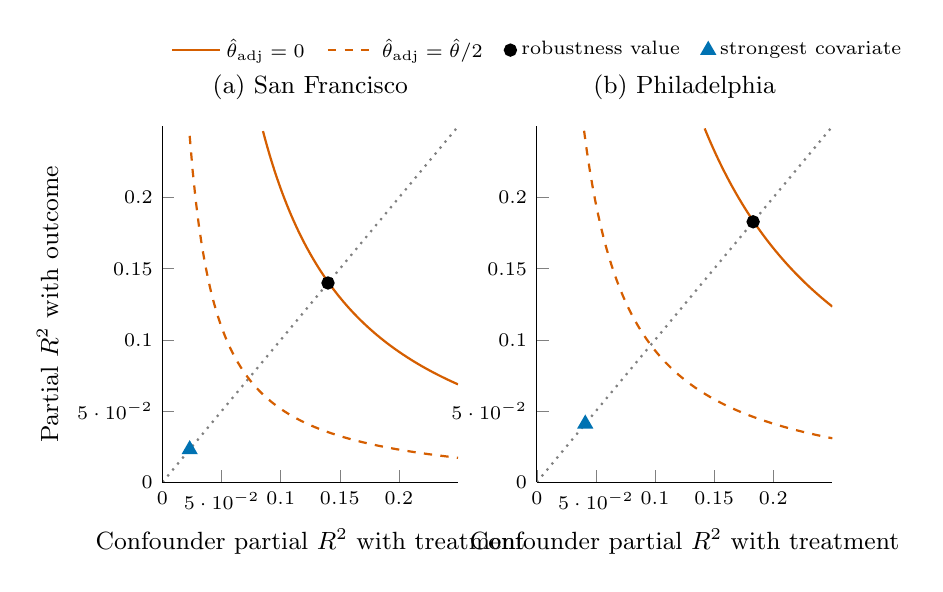
\begin{tikzpicture}
\begin{axis}[
    causalre, name=scA, width=0.44\textwidth, height=6.1cm,
    xlabel={Confounder partial $R^2$ with treatment},
    ylabel={Partial $R^2$ with outcome},
    xmin=0, xmax=0.25, ymin=0, ymax=0.25,
    xtick={0,0.05,0.10,0.15,0.20}, ytick={0,0.05,0.10,0.15,0.20},
    title={(a) San Francisco}, title style={font=\small},
    legend style={font=\scriptsize, draw=none, fill=none,
                  at={(0.0,1.15)}, anchor=south west, legend columns=4,
                  /tikz/every even column/.append style={column sep=6pt}},
]
\addplot[gray, dotted, thick, domain=0:0.25, forget plot] {x};
\addplot[cSF, thick, domain=0.085:0.25, samples=90] {0.02292*(1-x)/x};
\addlegendentry{$\hat\theta_{\mathrm{adj}}=0$}
\addplot[cSF, dashed, domain=0.023:0.25, samples=90] {0.00573*(1-x)/x};
\addlegendentry{$\hat\theta_{\mathrm{adj}}=\hat\theta/2$}
\addplot[only marks, mark=*, mark size=2pt, color=black] coordinates {(0.140,0.140)};
\addlegendentry{robustness value}
\addplot[only marks, mark=triangle*, mark size=2.6pt, color=cNYC] coordinates {(0.023,0.023)};
\addlegendentry{strongest covariate}
\end{axis}
\begin{axis}[
    causalre, width=0.44\textwidth, height=6.1cm,
    at={(scA.east)}, anchor=west, xshift=1.0cm,
    xlabel={Confounder partial $R^2$ with treatment}, ylabel={},
    xmin=0, xmax=0.25, ymin=0, ymax=0.25,
    xtick={0,0.05,0.10,0.15,0.20}, ytick={0,0.05,0.10,0.15,0.20},
    title={(b) Philadelphia}, title style={font=\small},
]
\addplot[cSF, thick, domain=0.142:0.25, samples=90] {0.04114*(1-x)/x};
\addplot[cSF, dashed, domain=0.040:0.25, samples=90] {0.01029*(1-x)/x};
\addplot[gray, dotted, thick, domain=0:0.25] {x};
\addplot[only marks, mark=*, mark size=2pt, color=black] coordinates {(0.183,0.183)};
\addplot[only marks, mark=triangle*, mark size=2.6pt, color=cNYC] coordinates {(0.041,0.041)};
\end{axis}
\end{tikzpicture}
\caption{Omitted-variable-bias sensitivity contours, in the manner of
\citet{cinelli2020making}, for the two markets that clear the robustness
threshold. The axes are the partial $R^2$ that a single unobserved confounder
would have with the treatment (horizontal) and with the outcome (vertical). The
solid curve is the locus along which such a confounder would drive the
per-standard-deviation estimate to zero, and the dashed curve the locus along
which it would halve it. The black dot, where the solid curve meets the dotted
equal-strength diagonal, is the robustness value, the equal-strength confounder
that just eliminates the effect, at $0.14$ in San Francisco and $0.18$ in
Philadelphia. The triangle marks a confounder as strong
as the most influential covariate actually observed, which falls far inside the
kill curve in both markets, so an unobserved confounder would have to be several
times stronger than any measured one to overturn the estimate.}
\label{fig:sensitivity-contour}
\end{figure}

\paragraph{Spatial-block leave-one-out.} Dropping the spatial control block and
re-estimating moves the point estimate by at most four thousandths of a log point
in any of the twelve markets, the largest shift falling in Phoenix at $+0.004$
and the rest smaller still. That the estimates barely respond to removing the
location controls is the pattern one would hope to see if the text signal were not
merely spatial information re-expressed, since a coefficient that rode on
geography would collapse once geography left the conditioning set rather than hold
to within Monte Carlo noise of where it began. The leave-one-out thus localizes,
market by market, the conclusion that the deconfounding decomposition of
Section~\ref{sec:decomposition} reaches for the embedding channel as a whole.

\paragraph{Fragility.} Under the same benchmarking convention a market is flagged
when the partial $R^2$ that the spatial block carries for either the treatment or
the outcome exceeds that market's robustness value, the condition under which a
confounder no stronger than the location controls already in the model could in
principle account for the estimate. Only Boston trips the flag, and it does so
because its robustness value is itself almost zero, the spatial block's
explanatory power for the treatment, at $0.012$, edging past a robustness value of
$0.005$ for an estimate that is statistically indistinguishable from zero to begin
with. No market with a robustness value above $0.025$ is flagged, so the fragility
check isolates the one place where there is no effect to confound rather than
casting doubt on any market where an effect is present.

\paragraph{Interpretation.} The analysis is deliberately confined to the single
observed covariate group the per-market panels share and the one most tied to the
mechanism this paper studies, so the robustness value carries the general bound
while the spatial leave-one-out localizes how much of each estimate rides on
measured location. The two diagnostics agree with each other and with the rest of
the section. Philadelphia and San Francisco, the markets in which the text effect
is largest, are also the ones most robust to unobserved confounding; the markets
that fall below the threshold are those whose estimates are already small; and
removing the explicit location controls disturbs none of them. We read the
per-market sensitivities as informative about robustness rather than as a second
identification test, and we leave the benchmarking of non-spatial confounder
groups to future work, since the census, crime, and amenity blocks needed to
construct them are not uniformly available across the twelve per-market panels.

\begin{figure}[H]
\centering
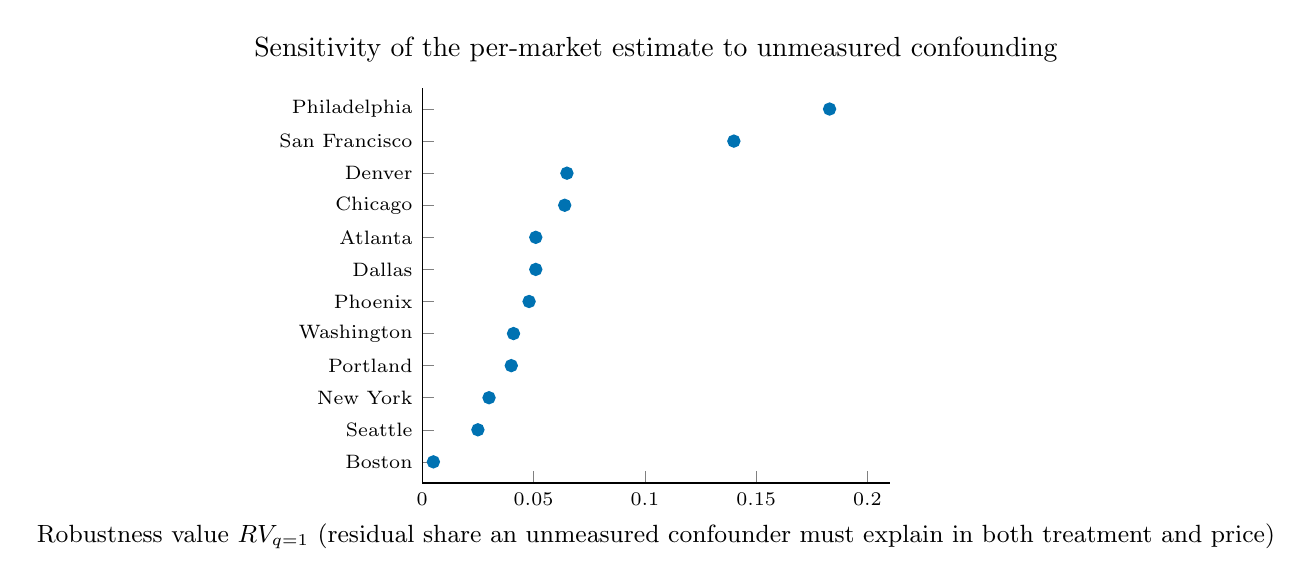
\begin{tikzpicture}
\begin{axis}[
    causalre, width=0.62\textwidth, height=6.6cm,
    symbolic y coords={Boston,Seattle,New York,Portland,Washington,Phoenix,Dallas,Atlanta,Chicago,Denver,San Francisco,Philadelphia},
    ytick=data, enlarge y limits=0.06,
    xlabel={Robustness value $RV_{q=1}$ (residual share an unmeasured confounder must explain in both treatment and price)},
    xmin=0, xmax=0.21, xtick={0,0.05,0.10,0.15,0.20},
    xticklabel={\pgfmathprintnumber[fixed,precision=2]{\tick}},
    title={Sensitivity of the per-market estimate to unmeasured confounding},
]
\addplot[only marks, mark=*, mark size=2.0pt, color=cNYC] coordinates {
  (0.005,Boston) (0.025,Seattle) (0.030,New York) (0.040,Portland) (0.041,Washington)
  (0.048,Phoenix) (0.051,Dallas) (0.051,Atlanta) (0.064,Chicago) (0.065,Denver)
  (0.140,San Francisco) (0.183,Philadelphia)};
\end{axis}
\end{tikzpicture}
\caption{Robustness value for each market's sentence-BERT effect, the share of
residual variance an unmeasured confounder would need to explain in both the
treatment and log price to drive the estimate to zero, following
\citet{cinelli2020making}. Larger values are more robust. The estimate is most
robust in Philadelphia ($0.18$) and San Francisco ($0.14$) and most fragile in
the markets whose point estimates are already near zero. The modest robustness
values in several markets are the reason we read the per-market estimates as
associational and sensitivity-bounded rather than cleanly causal.}
\label{fig:sensitivity-rv}
\end{figure}

\subsection{A composition-and-conditioning audit for text-treatment DML}
\label{sec:coca}

The robustness values of Table~\ref{tab:confounder-sensitivity-12} benchmark the
strength an unobserved confounder would need against the strength of the strongest
confounder we do observe, following \citet{cinelli2020making}. That benchmark has a
blind spot that a text-derived treatment walks directly into, and this section
names it, bounds it, and turns it into a pre-registered diagnostic.

Consider an omitted categorical covariate $C$, property type being the concrete
instance and vacant land the sharpest case, with three properties that hold in the
data. It shifts the treatment, $R^2_{T \sim C \mid X} > 0$, because a vacant lot is
described in different language than a house. It shifts price net of the treatment
and the observed controls, $R^2_{Y \sim C \mid T, X} > 0$. And it is nearly
invisible to the observed confounder block, $R^2(C \mid X) \approx 0$: a
cross-fitted classifier of the vacant-land indicator on the full confounder set
runs at an AUC of $0.50$ in Boston and $0.47$ in New York, while the same indicator
is recovered from the text direction at an AUC above $0.95$. The nearest-parcel
join that supplies the structured controls cannot represent landness, since for a
vacant lot it returns a neighbouring built parcel's attributes, so the design is
blind to exactly the attribute the text encodes. The bias from omitting such a $C$
is bounded by the partial-$R^2$ omitted-variable-bias inequality of
\citet{cinelli2020making} and its double-machine-learning generalization in
\citet{chernozhukov2022long}, and that bound holds whether or not $C$ is orthogonal
to $X$. What the orthogonality changes is not the bound but the benchmark used to
fill it in.

\begin{proposition}[Orthogonal composition defeats the observed-covariate benchmark]
\label{prop:coca}
In the partially-linear model of Equation~\eqref{eq:plr}, let $C$ be an omitted
covariate with $r_D := R^2_{T \sim C \mid X} > 0$ and
$r_Y := R^2_{Y \sim C \mid T, X} > 0$, and suppose $R^2(C \mid X) \to 0$. Then (i)
the protective subtraction that conditioning on $X$ applies to a confounder
correlated with the controls, the cross term $\rho_{TX}\rho_{CX}$ in the partial
correlation, vanishes, so the partial strengths $r_D$ and $r_Y$ that enter the
\citet{cinelli2020making} and \citet{chernozhukov2022long} bias bound are not
shrunk below their raw values, with $r_D \to R^2_{T \sim C}/(1 - R^2_{T \sim X})$ in
the limit; and (ii) the
observed-covariate benchmark, which calibrates the plausible magnitude of $C$ by
that of the strongest observed covariate, carries no warrant, because $C$ by
construction carries information orthogonal to the covariate space on which that
benchmark is computed. The robustness value reported against the observed benchmark
is therefore numerically well defined but uninformative about $C$.
\end{proposition}

The argument is short. Partialling $X$ out of $T$ and of $C$ leaves residuals whose
correlation obeys the recursive identity
$\rho_{TC \mid X} = (\rho_{TC} - \rho_{TX}\rho_{CX}) /
\sqrt{(1 - \rho_{TX}^2)(1 - \rho_{CX}^2)}$, whose protective subtraction
$\rho_{TX}\rho_{CX}$ vanishes as $\mathrm{Cor}(C, X) \to 0$, leaving
$\rho_{TC \mid X} \to \rho_{TC} / \sqrt{1 - \rho_{TX}^2}$, no smaller than the raw
correlation; the same holds on the outcome side, which gives part (i). A computer-
algebra check confirms both this identity and the fact that for a single omitted
confounder the \citet{cinelli2020making} bias expression equals the exact bias
rather than merely bounding it, so the bound the audit reasons about is tight; the
verification is released with the replication code. Part (ii)
is the operational reading: the benchmark's premise is that an omitted confounder
is comparable in strength to an observed covariate, and a classifier of $C$ on $X$
running at chance is direct evidence that $C$ lives outside the space that premise
is calibrated on. We are careful about what this does and does not establish. It is
not that the formal bound cannot detect $C$; \citet{cinelli2020making} show in
their own Section~6.2 that the correctly computed bound recovers the right answer
for a confounder orthogonal to the controls when the analyst sets the benchmark
strength correctly. It is that the routine heuristic of setting that strength by
analogy to observed covariates has no anchor once $R^2(C \mid X) \approx 0$, and
this is precisely the regime in which an analyst is most likely to feel wrongly
reassured, since orthogonal to the controls reads too easily as weak. The claim in
part (i) that conditioning shrinks a correlated confounder's residual strength is
generic rather than universal, since \citet{middleton2016bias} show that
conditioning on covariates correlated with an unobserved confounder can amplify
rather than shrink the bias in bad-control configurations, so it is the expected
case and not a law.

A second, distinct failure channel travels with the first. When $C$ nearly sorts
the treatment, the residual treatment variance $E[(T - E[T \mid X, C])^2]$
collapses and the orthogonal score becomes ill conditioned, a phenomenon
\citet{saco2025illconditioned} characterize through the conditioning number
$\kappa = 1/(1 - R^2_{\text{oof}}(T \mid X))$; that reference reports the diagnostic
as a fragility assessment and deliberately proposes no universal threshold, and we
follow it in treating $\kappa$ and the design-matrix condition number as flags read
alongside the substantive analysis rather than as a test. The composition confound
and the conditioning degeneracy are separate objects, and confusing one for the
other misdiagnoses the fix: the first is corrected by adjusting for the omitted
category, the second by repairing the design.

These two channels motivate a two-step audit, run before the point estimate is
inspected, that we call the composition-and-conditioning audit. Step one screens
conditioning: flag a market if the standardized confounder matrix has condition
number above $10^6$ or any confounder column has collapsed to a constant, either of
which signals a design-matrix degeneracy rather than a treatment effect. Step two
screens composition: flag a market if a candidate omitted category is
chance-predictable from the controls, $\mathrm{AUC}(C \mid X) < 0.60$, yet strongly
predictable from the treatment, $\mathrm{AUC}(C \mid T) > 0.75$. The prescribed
correction differs by step. A conditioning flag is a pipeline repair. A composition
flag calls for adjusting for the category, and the natural instinct, adding a
property-type dummy to the regularized nuisance, backfires, because the ridge
penalty shrinks a rare category toward no effect: in Boston, where non-residential
listings are $1.9\%$ of the sample, adding the dummy raises $|\hat\theta|$ from
$0.40$ to $0.45$. Exact within-category demeaning of the treatment and the outcome,
which is unpenalized, is the correct adjustment and lowers the Boston estimate to
$0.34$. Across the panel the composition adjustment materially moves only the two
markets with the largest non-residential share, Philadelphia and Chicago, and
leaves the rest, including the New York exception, essentially unchanged, which is
consistent with the mechanism the proposition describes.

A calibration study confirms that the two steps discriminate the two failure modes
rather than firing together. Across a grid of category shares and confounder
strengths, with $200$ replications per cell, the conditioning step fires on a
simulated design degeneracy in every replication and never on a composition
confound, while the composition step fires on a material composition confound, one
strong enough to lift $\mathrm{AUC}(C \mid T)$ above the threshold, in more than
nine of ten replications and never on a design degeneracy; the false-positive rate
of each step on the other's failure mode is zero. The audit therefore separates a
numerical artifact from a substantive confound on data the analysis already has,
and it does so before the estimate is read, which is what a pre-registered
diagnostic is meant to do. We claim for it neither a new estimator nor a new limit
theorem, only the connection of two existing literatures, the omitted-variable-bias
bounds of \citet{cinelli2020making} and \citet{chernozhukov2022long} and the
conditioning diagnostics of \citet{saco2025illconditioned}, into a screen fitted to
the specific way a text-derived treatment fails.


\subsection{Cross-market heterogeneity and a null moderator}
\label{sec:meta-regression-12}

The twelve per-market estimates are heterogeneous, ranging from a small negative in
New York to several times the mean in Chicago and Philadelphia, so a pooled figure
summarizes a dispersed distribution rather than a single generalizable effect.
Combining the markets by inverse-variance weighting, the Shen-Ross uniqueness
channel pools to $+0.060$ with a $95\%$ interval of $[+0.018, +0.102]$ and the
sentence-BERT axis, under the price-positive orientation of
Section~\ref{sec:baur-12city}, to $+0.137$ with $[+0.048, +0.227]$. Both channels
are positive and detectable in the pool, and the conclusion is stable across the
weighting choice: weighting each market equally and weighting by sample size return
Baur pooled estimates of $+0.137$ and $+0.130$, and the precision-weighted value is
$+0.122$, the gap reflecting only that New York carries a fifth of the listings at a
small negative effect, so that dropping it lifts the market-weighted mean to
$+0.152$. What moves the pool is the single market the rest of the paper already
isolates.

We looked for a metropolitan-level moderator of the effect and found none.
Regressing each channel's per-market estimate on eleven metropolitan covariates,
eight from the American Community Survey and three from federal series, no covariate
reaches nominal significance on either channel; the renter share of the housing
stock carries the smallest raw $p$, at $0.074$ on the Baur channel, and survives
neither multiplicity adjustment nor the leave-one-out influence diagnostics. With
twelve markets a regression on site-level estimates is underpowered by construction,
so the honest reading is the absence of a moderator detectable at this sample size
rather than a demonstrated absence of moderation, and a properly powered treatment
would carry the covariate as an interaction in a stacked specification rather than a
regression on twelve site estimates. We record one correction. An earlier draft
reported a positive and significant renter-share moderator, which turned out to be
produced by a corrupted confounder in a single market that the winsorization of
Section~\ref{sec:data} removes; once corrected, the coefficient reverses sign and
loses significance, and we report the null rather than carry the superseded claim.

% §6.7 Cross-method orthogonality between Shen, Baur, and counterfactual.
% Numbers locked against results/replications/cross_method_concordance.csv
% and hotelling_t2_cross_method.csv (both refreshed with the clean CF run).
% Spearman and sign-agreement computed on the per-city point estimates.
% Clean k=12, no Portland exclusion. The v2 "joint factor model" subsection
% (lambda/sigma values, 12/12 credible intervals) had no backing file and is
% removed; a latent one-factor pooling is noted as planned future work only.

\subsection{Cross-method orthogonality}
\label{sec:cross-method-12}

Sections~\ref{sec:shen-12city} and~\ref{sec:baur-12city} each identify
a different small subset of metropolitan markets in which a
text-on-price effect can be detected at conventional significance. The
natural question is whether the channels agree on which markets carry
an effect, or whether they capture substantively different aspects of
listing language. We answer it by computing per-market rank and sign
correlations between the Shen-Ross uniqueness DML estimate and the
Baur PC1 DML estimate, and we add the counterfactual rewriting total
effect from Section~\ref{sec:counterfactual-12} as a third axis.

\paragraph{Pairwise rank correlations.}
Table~\ref{tab:cross-method-12} reports the per-market point estimates
for the three channels. Across the twelve markets the Spearman rank
correlation between the Shen-Ross estimate and the counterfactual
total effect is $+0.64$ ($p = 0.02$), the strongest of the three
pairings, while the correlation between the Shen-Ross estimate and the
Baur estimate is $-0.59$ ($p = 0.05$) and the correlation between the
Baur estimate and the counterfactual total effect is $-0.52$
($p = 0.09$). With only twelve markets the rank statistic carries a
standard error near $1/\sqrt{12} \approx 0.29$, so we read these
coefficients as descriptive of the cross-market pattern rather than as
precise estimates of agreement. The pattern that emerges is that the
Shen uniqueness channel and the counterfactual-rewriting channel rank
together across markets, whereas the Baur PC1 axis ranks oppositely to
both, which is the direction expected from its negative pooled loading
on the utilitarian-vocabulary axis documented in
Section~\ref{sec:baur-12city}: a market with a strongly positive
Shen uniqueness premium tends to sit low on the Baur axis. We do not
read the negative Baur correlations as evidence that the channels
contradict one another, because the channels are measured on axes with
opposite substantive orientation.

\paragraph{Sign agreement.} Counting markets in which two channels
share the sign of their point estimate, the Shen and counterfactual
channels agree in seven of the twelve markets, the strongest pairwise
sign concordance and consistent with their positive rank correlation,
while Shen and Baur agree in three markets and Baur and the
counterfactual agree in two. No market has all three channels sharing
a common sign, which again reflects the opposite orientation of the
Baur axis rather than methodological inconsistency.

\paragraph{Identification overlap.} A more decision-relevant summary
than rank agreement is which markets each channel identifies at the
$95\%$ level, where the per-method bootstrap confidence interval
excludes zero. The Shen channel identifies ten of the twelve markets,
the counterfactual channel nine, and the Baur axis four, namely New
York, Philadelphia, Denver, and Atlanta, all of which also clear the
Shen threshold. Three markets are identified by all three channels
jointly, New York, Philadelphia, and Denver, and eight of the twelve
are identified by at least two channels, with no market left
unidentified by every channel. Among the markets identified by
exactly two channels, four pair the Shen and counterfactual axes, San
Francisco, Washington DC, Phoenix, and Dallas, and one pairs Shen and
Baur, Atlanta, which mirrors the positive Shen-counterfactual rank
correlation at the level of the identified set.

\paragraph{Substantive interpretation under a triangulation design.}
The three identification strategies are not redundant point estimators
of a single scalar effect; they are deliberately chosen to have
orthogonal sources of bias. The Shen-Ross uniqueness measure leverages
within-market lexical rarity and inherits any bias from the
neighborhood-peer-set definition, the Baur sentence-BERT axis
leverages cross-listing semantic geometry and inherits bias from the
embedding model's pretraining distribution, and the LLM counterfactual
rewriting intervention leverages within-listing minimal-edit
substitution and inherits bias from the rewriter's distributional
shift. Following the causal-triangulation framework of
\citet{lawlor2016triangulation} and \citet{hammerton2021causal},
methods whose biases are largely unrelated provide jointly stronger
evidence on a common causal target than methods that share a bias
structure, regardless of whether their per-market point estimates
agree numerically. This is a per-market restatement of the
\citet{heckman2008econometric} position that different estimators
identify different parameters: each method rejects a method-specific
null about a method-specific functional of the language-price
relationship, while the joint test below rejects the global null that
no functional has any effect in a given market. Under this design the
mixed and imprecise pairwise correlations are the discriminant-validity
signal the design anticipates, and the joint rejection pattern is the
convergent signal, which is the canonical signature predicted when
several low-power estimators each identify a different feature of a
partially-identified estimand \citep{manski2003partial, tamer2010partial}:
the joint test inherits power from the union of identifying
restrictions even when each marginal test does not.

\paragraph{Joint-null Hotelling test.} The most powerful summary of
the cross-method evidence asks, for each market, whether the joint null
$H_0: (\theta_{\mathrm{Shen}}, \theta_{\mathrm{Baur}},
\theta_{\mathrm{CF}}) = (0, 0, 0)$ can be rejected against the
two-sided alternative. Treating the three per-market estimates as
asymptotically independent, since the three methods use disjoint
sources of variation in a Doc2Vec uniqueness score, a sentence-BERT
principal component, and an LLM-rewriting differential, we compute the
Hotelling-style statistic $T^2_m = z^2_{\mathrm{Shen},m} +
z^2_{\mathrm{Baur},m} + z^2_{\mathrm{CF},m}$ per market and refer it to
a $\chi^2_3$ asymptotic distribution. The joint null is rejected in all
twelve of the twelve markets at conventional five-percent significance,
and the rejection survives Benjamini-Hochberg false-discovery
correction across the twelve markets, where the largest adjusted
$q$-value is $0.002$. The weakest joint rejection is Boston, with
$T^2 = 14.5$ and $q = 0.002$, and even there the joint null is
comfortably rejected, so the post-2020 panel contains no market that
reads as a clean text-on-price null. Atlanta, which an earlier draft
treated as a clean null, now rejects strongly with $T^2 = 128$ on the
strength of its Shen and Baur $z$-statistics even though its
counterfactual interval covers zero. The rejection of the joint null
in every market despite the mixed and imprecise pairwise rank
correlations is consistent with each method contributing independent
low-power evidence of a non-zero text-on-price signal, even when no
single method attains significance on that market alone.

We favor the reading that text-on-price effects are real but
heterogeneous across metropolitan markets, with the channel that
detects an effect varying by market, while leaving open the question of
which method is preferred when an analyst can deploy only one. A
constructive complement to the joint Hotelling test would treat the
three per-market estimates as noisy indicators of a single latent
market-level text-price effect and pool them through an anchored
one-factor measurement model in the tradition of latent-variable
meta-analysis, recovering a precision-weighted posterior for each
market's common factor. We have not fit that model on the present
panel and report it here only as a planned extension, so the joint
Hotelling test and the identification-overlap counts above remain the
cross-method evidence on which the conclusions of this section rest.

% v3 figures, AOAS reframe. PURE TikZ/pgfplots, matching the house `causalre`
% style (Tufte axis lines*=left, Okabe-Ito palette, manual gray CI whiskers,
% extra-tick dashed null lines, consistent marks). Coordinates emitted from
% results/ by data/scripts/make_fig_coords.py (no manual transcription).
% Figures: coverage sim, per-market forest, LEACE erasure, sensitivity (RV),
% concordance (supplement). Decomposition figure pending the pre/post-LEACE
% price re-estimate (see note at end of file).

% ======================================================================
% FIG: finite-sample coverage of the embedding-treatment DML interval
% data: results/simulation_baseline/coverage_table.csv
% ======================================================================
\begin{figure}[!htbp]
\centering
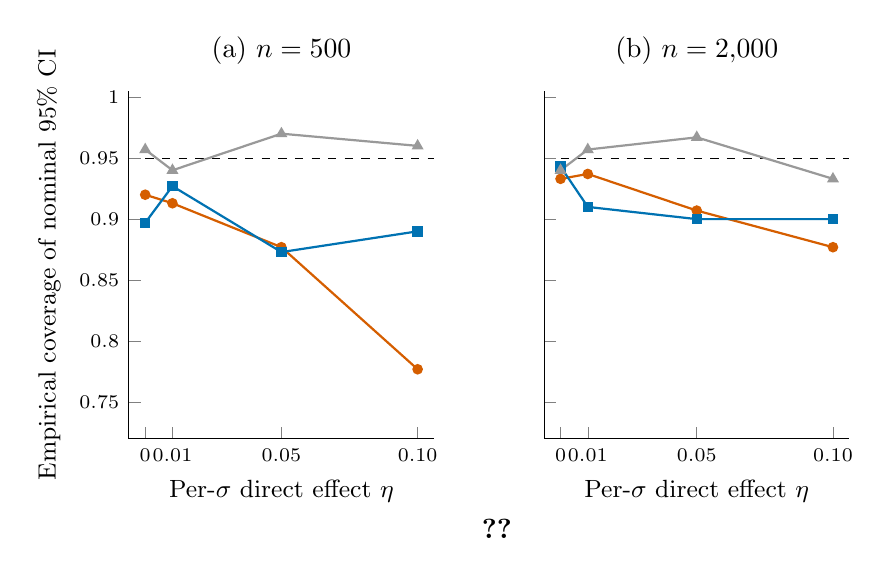
\begin{tikzpicture}
\begin{axis}[
    causalre body, name=covA,
    xlabel={Per-$\sigma$ direct effect $\eta$},
    ylabel={Empirical coverage of nominal $95\%$ CI},
    title={(a) $n = 500$},
    xmin=-0.006, xmax=0.106, ymin=0.72, ymax=1.005,
    xtick={0,0.01,0.05,0.10}, xticklabels={$0$,$0.01$,$0.05$,$0.10$},
    ytick={0.75,0.80,0.85,0.90,0.95,1.00},
    legend to name=covleg, legend columns=3,
    legend style={font=\scriptsize, draw=none, fill=none,
                  /tikz/every even column/.append style={column sep=12pt}},
    legend cell align=left,
]
\addplot[black, dashed, thin, forget plot] coordinates {(-0.006,0.95) (0.106,0.95)};
\addplot[color=cSF,  thick, mark=*,         mark size=1.5pt] coordinates {(0,0.920) (0.01,0.913) (0.05,0.877) (0.10,0.777)};
\addlegendentry{DML (in-sample PC)}
\addplot[color=cNYC, thick, mark=square*,   mark size=1.5pt] coordinates {(0,0.897) (0.01,0.927) (0.05,0.873) (0.10,0.890)};
\addlegendentry{DML (cross-fit PC)}
\addplot[color=cBOS, thick, mark=triangle*, mark size=1.7pt] coordinates {(0,0.957) (0.01,0.940) (0.05,0.970) (0.10,0.960)};
\addlegendentry{Doubly robust}
\end{axis}
\begin{axis}[
    causalre body,
    at={(covA.east)}, anchor=west, xshift=1.4cm,
    xlabel={Per-$\sigma$ direct effect $\eta$}, ylabel={},
    title={(b) $n = 2{,}000$},
    xmin=-0.006, xmax=0.106, ymin=0.72, ymax=1.005,
    xtick={0,0.01,0.05,0.10}, xticklabels={$0$,$0.01$,$0.05$,$0.10$},
    ytick={0.75,0.80,0.85,0.90,0.95,1.00}, yticklabels={,,,,,},
]
\addplot[black, dashed, thin, forget plot] coordinates {(-0.006,0.95) (0.106,0.95)};
\addplot[color=cSF,  thick, mark=*,         mark size=1.5pt, forget plot] coordinates {(0,0.933) (0.01,0.937) (0.05,0.907) (0.10,0.877)};
\addplot[color=cNYC, thick, mark=square*,   mark size=1.5pt, forget plot] coordinates {(0,0.943) (0.01,0.910) (0.05,0.900) (0.10,0.900)};
\addplot[color=cBOS, thick, mark=triangle*, mark size=1.7pt, forget plot] coordinates {(0,0.940) (0.01,0.957) (0.05,0.967) (0.10,0.933)};
\end{axis}
\node[anchor=north] at ($(covA.south east)+(0.8cm,-0.9cm)$) {\ref{covleg}};
\end{tikzpicture}
\caption{Finite-sample coverage of the nominal $95\%$ influence-function interval
for the embedding-valued treatment, across effect size $\eta$ at $n=500$ (a) and
$n=2{,}000$ (b), with $300$ Monte Carlo replications per cell. The horizontal
dashed line marks the nominal level. The in-sample principal-component DML
interval, which treats the estimated leading component as a generated regressor,
under-covers as the true effect grows, falling to $0.78$ at $n=500$, because the
orthogonal-score variance does not capture the sampling variability of the
estimated treatment direction. Forming the component out of fold (cross-fit PC)
recovers most of the lost coverage, and the doubly-robust estimator, which does
not estimate a continuous direction, is calibrated throughout but has no power
against the graded effect.}
\label{fig:sim-coverage}
\end{figure}

% ======================================================================
% FIG: per-market forest, three text channels (12 metros)
% data: shen_12city_table / baur_pooled_pca_table / counterfactual_12city_table
% rows ordered by Shen effect (idx 1 = bottom). Gray whiskers + filled dots.
% ======================================================================
\begin{figure}[!htbp]
\centering
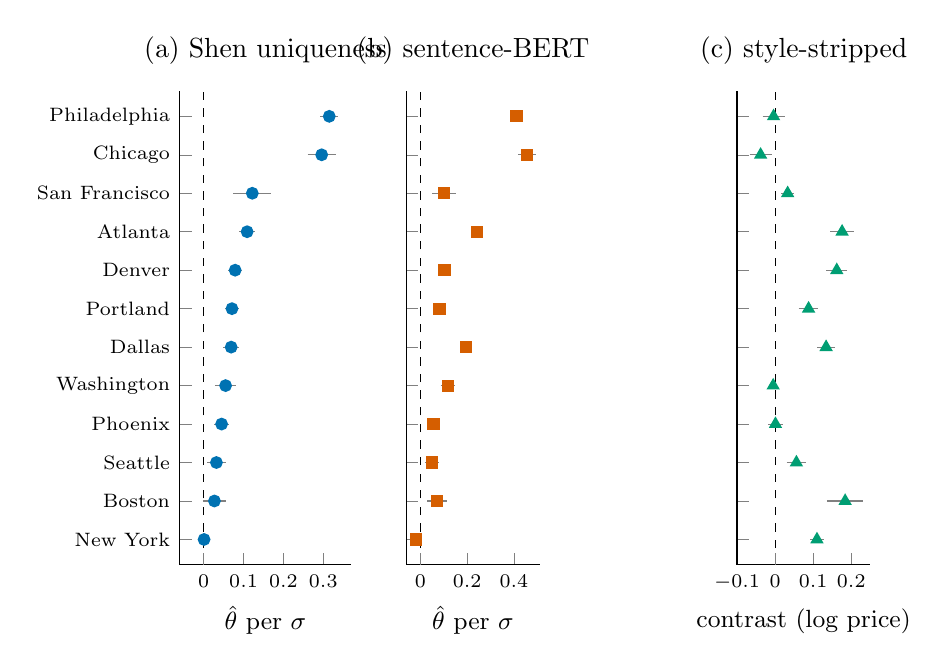
\begin{tikzpicture}
% --- panel (a) Shen uniqueness ---
\begin{axis}[
    causalre, width=0.31\textwidth, height=7.6cm, name=fsA,
    symbolic y coords={New York,Boston,Seattle,Phoenix,Washington,Dallas,Portland,Denver,Atlanta,San Francisco,Chicago,Philadelphia},
    ytick=data, y dir=normal,
    xlabel={$\hat\theta$ per $\sigma$}, xmin=-0.06, xmax=0.37,
    xtick={0,0.1,0.2,0.3}, enlarge y limits=0.06,
    title={(a) Shen uniqueness},
    extra x ticks={0}, extra x tick style={grid=major, grid style={black, dashed, thin}}, extra x tick labels={},
]
\draw[thin,gray] (axis cs:-0.011,New York)--(axis cs:0.013,New York);
\draw[thin,gray] (axis cs:-0.002,Boston)--(axis cs:0.056,Boston);
\draw[thin,gray] (axis cs:0.009,Seattle)--(axis cs:0.055,Seattle);
\draw[thin,gray] (axis cs:0.027,Phoenix)--(axis cs:0.063,Phoenix);
\draw[thin,gray] (axis cs:0.028,Washington)--(axis cs:0.082,Washington);
\draw[thin,gray] (axis cs:0.049,Dallas)--(axis cs:0.089,Dallas);
\draw[thin,gray] (axis cs:0.053,Portland)--(axis cs:0.089,Portland);
\draw[thin,gray] (axis cs:0.062,Denver)--(axis cs:0.096,Denver);
\draw[thin,gray] (axis cs:0.089,Atlanta)--(axis cs:0.129,Atlanta);
\draw[thin,gray] (axis cs:0.074,San Francisco)--(axis cs:0.170,San Francisco);
\draw[thin,gray] (axis cs:0.261,Chicago)--(axis cs:0.331,Chicago);
\draw[thin,gray] (axis cs:0.292,Philadelphia)--(axis cs:0.338,Philadelphia);
\addplot[only marks, mark=*, mark size=1.9pt, color=cNYC] coordinates {
  (0.001,New York) (0.027,Boston) (0.032,Seattle) (0.045,Phoenix) (0.055,Washington)
  (0.069,Dallas) (0.071,Portland) (0.079,Denver) (0.109,Atlanta) (0.122,San Francisco)
  (0.296,Chicago) (0.315,Philadelphia)};
\end{axis}
% --- panel (b) Baur sentence-BERT axis ---
\begin{axis}[
    causalre, width=0.27\textwidth, height=7.6cm,
    at={(fsA.east)}, anchor=west, xshift=0.7cm,
    symbolic y coords={New York,Boston,Seattle,Phoenix,Washington,Dallas,Portland,Denver,Atlanta,San Francisco,Chicago,Philadelphia},
    ytick=data, yticklabels={,,,,,,,,,,,},
    xlabel={$\hat\theta$ per $\sigma$}, xmin=-0.06, xmax=0.51,
    xtick={0,0.2,0.4}, enlarge y limits=0.06,
    title={(b) sentence-BERT},
    extra x ticks={0}, extra x tick style={grid=major, grid style={black, dashed, thin}}, extra x tick labels={},
]
\draw[thin,gray] (axis cs:-0.033,New York)--(axis cs:-0.005,New York);
\draw[thin,gray] (axis cs:0.029,Boston)--(axis cs:0.115,Boston);
\draw[thin,gray] (axis cs:0.019,Seattle)--(axis cs:0.079,Seattle);
\draw[thin,gray] (axis cs:0.030,Phoenix)--(axis cs:0.082,Phoenix);
\draw[thin,gray] (axis cs:0.087,Washington)--(axis cs:0.149,Washington);
\draw[thin,gray] (axis cs:0.175,Dallas)--(axis cs:0.215,Dallas);
\draw[thin,gray] (axis cs:0.057,Portland)--(axis cs:0.107,Portland);
\draw[thin,gray] (axis cs:0.084,Denver)--(axis cs:0.122,Denver);
\draw[thin,gray] (axis cs:0.220,Atlanta)--(axis cs:0.266,Atlanta);
\draw[thin,gray] (axis cs:0.051,San Francisco)--(axis cs:0.151,San Francisco);
\draw[thin,gray] (axis cs:0.419,Chicago)--(axis cs:0.493,Chicago);
\draw[thin,gray] (axis cs:0.390,Philadelphia)--(axis cs:0.432,Philadelphia);
\addplot[only marks, mark=square*, mark size=1.8pt, color=cSF] coordinates {
  (-0.019,New York) (0.072,Boston) (0.049,Seattle) (0.056,Phoenix) (0.118,Washington)
  (0.195,Dallas) (0.082,Portland) (0.103,Denver) (0.243,Atlanta) (0.101,San Francisco)
  (0.456,Chicago) (0.411,Philadelphia)};
\end{axis}
% --- panel (c) counterfactual style-stripped contrast ---
\begin{axis}[
    causalre, width=0.27\textwidth, height=7.6cm,
    at={(fsA.east)}, anchor=west, xshift=4.9cm,
    symbolic y coords={New York,Boston,Seattle,Phoenix,Washington,Dallas,Portland,Denver,Atlanta,San Francisco,Chicago,Philadelphia},
    ytick=data, yticklabels={,,,,,,,,,,,},
    xlabel={contrast (log price)}, xmin=-0.10, xmax=0.25,
    xtick={-0.1,0,0.1,0.2}, enlarge y limits=0.06,
    title={(c) style-stripped},
    extra x ticks={0}, extra x tick style={grid=major, grid style={black, dashed, thin}}, extra x tick labels={},
]
\draw[thin,gray] (axis cs:0.092,New York)--(axis cs:0.128,New York);
\draw[thin,gray] (axis cs:0.136,Boston)--(axis cs:0.232,Boston);
\draw[thin,gray] (axis cs:0.030,Seattle)--(axis cs:0.082,Seattle);
\draw[thin,gray] (axis cs:-0.018,Phoenix)--(axis cs:0.020,Phoenix);
\draw[thin,gray] (axis cs:-0.015,Washington)--(axis cs:0.005,Washington);
\draw[thin,gray] (axis cs:0.111,Dallas)--(axis cs:0.157,Dallas);
\draw[thin,gray] (axis cs:0.062,Portland)--(axis cs:0.114,Portland);
\draw[thin,gray] (axis cs:0.135,Denver)--(axis cs:0.189,Denver);
\draw[thin,gray] (axis cs:0.145,Atlanta)--(axis cs:0.207,Atlanta);
\draw[thin,gray] (axis cs:0.016,San Francisco)--(axis cs:0.050,San Francisco);
\draw[thin,gray] (axis cs:-0.067,Chicago)--(axis cs:-0.009,Chicago);
\draw[thin,gray] (axis cs:-0.033,Philadelphia)--(axis cs:0.025,Philadelphia);
\addplot[only marks, mark=triangle*, mark size=2.0pt, color=cGRN] coordinates {
  (0.110,New York) (0.184,Boston) (0.056,Seattle) (0.001,Phoenix) (-0.005,Washington)
  (0.134,Dallas) (0.088,Portland) (0.162,Denver) (0.176,Atlanta) (0.033,San Francisco)
  (-0.038,Chicago) (-0.004,Philadelphia)};
\end{axis}
\end{tikzpicture}
\caption{Per-market DML estimates across the twelve metropolitan areas for the
three text channels, ordered by the Shen-Ross uniqueness effect. Filled dots are
point estimates and gray whiskers are $95\%$ intervals (influence-function for
the Shen and sentence-BERT channels; coefficient-uncertainty-folded cluster
bootstrap for the counterfactual contrast). The dashed vertical line marks the
null. The sentence-BERT axis is oriented so its pooled effect is non-negative.
Numerical values appear in Tables~\ref{tab:shen-12city}, \ref{tab:baur-12city},
and \ref{tab:counterfactual-12}.}
\label{fig:forest-12}
\end{figure}

% ======================================================================
% FIG: LEACE erasure completeness (held-out ridge R^2 on lat-lon)
% data: results/leace12_igbp/leace_12city_table.csv, ordered by raw R^2
% dumbbell: gray segment raw->erased, open dot raw, filled dot erased
% ======================================================================
\begin{figure}[!htbp]
\centering
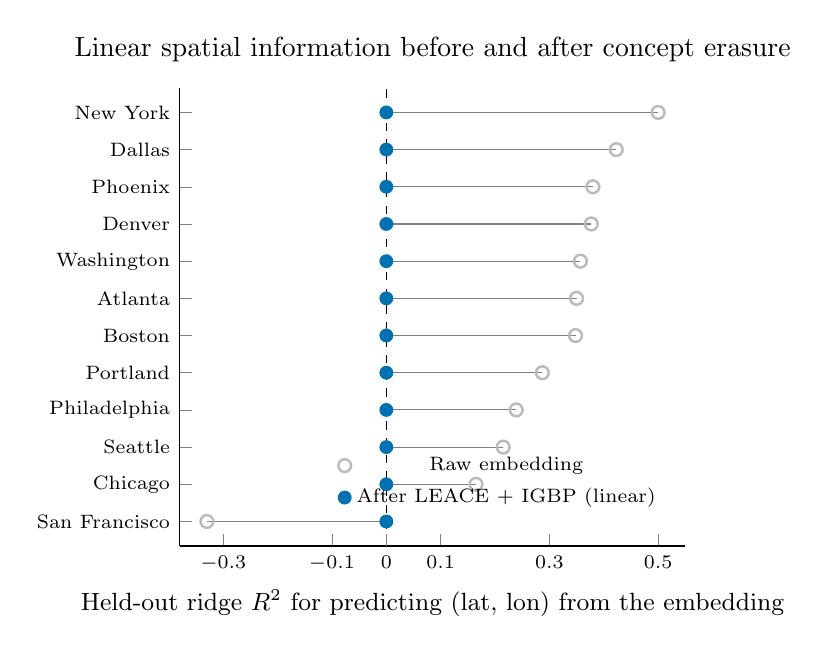
\begin{tikzpicture}
\begin{axis}[
    causalre, width=0.66\textwidth, height=7.4cm,
    symbolic y coords={San Francisco,Chicago,Seattle,Philadelphia,Portland,Boston,Atlanta,Washington,Denver,Phoenix,Dallas,New York},
    ytick=data, enlarge y limits=0.06,
    xlabel={Held-out ridge $R^2$ for predicting (lat, lon) from the embedding},
    xmin=-0.38, xmax=0.55, xtick={-0.3,-0.1,0,0.1,0.3,0.5},
    title={Linear spatial information before and after concept erasure},
    extra x ticks={0}, extra x tick style={grid=major, grid style={black, dashed, thin}}, extra x tick labels={},
    legend style={font=\scriptsize, draw=none, fill=none, at={(0.97,0.06)}, anchor=south east, row sep=1pt},
]
% raw -> erased connecting segments
\draw[thin,gray] (axis cs:-0.330,San Francisco)--(axis cs:0.000,San Francisco);
\draw[thin,gray] (axis cs:0.165,Chicago)--(axis cs:0.000,Chicago);
\draw[thin,gray] (axis cs:0.215,Seattle)--(axis cs:0.000,Seattle);
\draw[thin,gray] (axis cs:0.239,Philadelphia)--(axis cs:0.000,Philadelphia);
\draw[thin,gray] (axis cs:0.287,Portland)--(axis cs:0.000,Portland);
\draw[thin,gray] (axis cs:0.348,Boston)--(axis cs:0.000,Boston);
\draw[thin,gray] (axis cs:0.350,Atlanta)--(axis cs:0.000,Atlanta);
\draw[thin,gray] (axis cs:0.357,Washington)--(axis cs:0.000,Washington);
\draw[thin,gray] (axis cs:0.377,Denver)--(axis cs:0.000,Denver);
\draw[thin,gray] (axis cs:0.380,Phoenix)--(axis cs:0.000,Phoenix);
\draw[thin,gray] (axis cs:0.423,Dallas)--(axis cs:0.000,Dallas);
\draw[thin,gray] (axis cs:0.500,New York)--(axis cs:0.000,New York);
\addplot[only marks, mark=o, mark size=2.3pt, color=cMUTE, line width=0.9pt] coordinates {
  (-0.330,San Francisco) (0.165,Chicago) (0.215,Seattle) (0.239,Philadelphia) (0.287,Portland)
  (0.348,Boston) (0.350,Atlanta) (0.357,Washington) (0.377,Denver) (0.380,Phoenix)
  (0.423,Dallas) (0.500,New York)};
\addlegendentry{Raw embedding}
\addplot[only marks, mark=*, mark size=2.1pt, color=cNYC] coordinates {
  (0.000,San Francisco) (0.000,Chicago) (0.000,Seattle) (0.000,Philadelphia) (0.000,Portland)
  (0.000,Boston) (0.000,Atlanta) (0.000,Washington) (0.000,Denver) (0.000,Phoenix)
  (0.000,Dallas) (0.000,New York)};
\addlegendentry{After LEACE $+$ IGBP (linear)}
\end{axis}
\end{tikzpicture}
\caption{Held-out ridge $R^2$ for recovering the continuous latitude-longitude
coordinate from the sentence-BERT embedding, before (open) and after (filled)
the composed linear concept erasure, in each of the twelve markets ordered by raw
$R^2$. The raw embedding carries substantial linear spatial signal, recovering
the coordinate at $R^2$ up to $0.50$ in New York; the negative San Francisco
value reflects out-of-sample probe performance below the coordinate-mean
baseline rather than absent signal. Linear erasure drives the recoverable signal
to within Monte Carlo noise of zero in every market, the exact-guardedness
property of LEACE. Residual \emph{nonlinear} leakage, which a linear probe cannot
see, is quantified separately in Section~\ref{sec:leace-12}.}
\label{fig:erasure-12}
\end{figure}

% ======================================================================
% FIG: GRL adversarial erasure foil -- a fresh probe recovers location
% from the adversarially-deconfounded encoder but not from the LEACE projection
% data: results/adversarial_12city/adversarial_12city_summary.csv (geo_probe_r2)
% vs the LEACE linear-erased coordinate R2 (~0, fig:erasure-12)
% ======================================================================
\begin{figure}[!htbp]
\centering
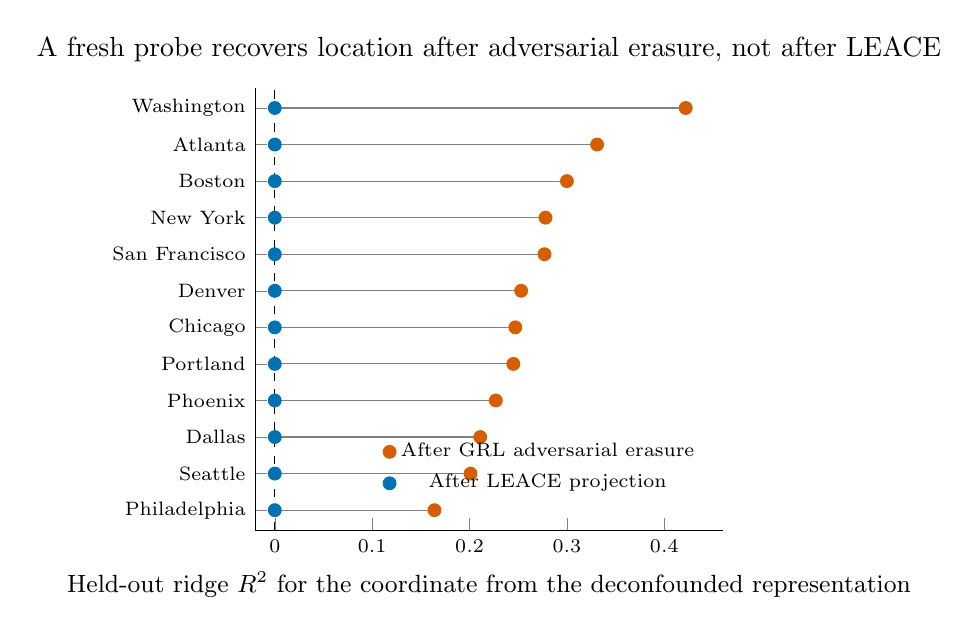
\begin{tikzpicture}
\begin{axis}[
    causalre, width=0.62\textwidth, height=7.2cm,
    symbolic y coords={Philadelphia,Seattle,Dallas,Phoenix,Portland,Chicago,
                       Denver,San Francisco,New York,Boston,Atlanta,Washington},
    ytick=data, enlarge y limits=0.05,
    xlabel={Held-out ridge $R^2$ for the coordinate from the deconfounded representation},
    xmin=-0.02, xmax=0.46, xtick={0,0.1,0.2,0.3,0.4},
    xticklabel={\pgfmathprintnumber[fixed,precision=1]{\tick}},
    title={A fresh probe recovers location after adversarial erasure, not after LEACE},
    extra x ticks={0}, extra x tick style={grid=major, grid style={black, dashed, thin}}, extra x tick labels={},
    legend style={font=\scriptsize, draw=none, fill=none, at={(0.97,0.06)}, anchor=south east, row sep=1pt},
]
\draw[thin,gray] (axis cs:0.164,Philadelphia)--(axis cs:0.000,Philadelphia);
\draw[thin,gray] (axis cs:0.201,Seattle)--(axis cs:0.000,Seattle);
\draw[thin,gray] (axis cs:0.211,Dallas)--(axis cs:0.000,Dallas);
\draw[thin,gray] (axis cs:0.227,Phoenix)--(axis cs:0.000,Phoenix);
\draw[thin,gray] (axis cs:0.245,Portland)--(axis cs:0.000,Portland);
\draw[thin,gray] (axis cs:0.247,Chicago)--(axis cs:0.000,Chicago);
\draw[thin,gray] (axis cs:0.253,Denver)--(axis cs:0.000,Denver);
\draw[thin,gray] (axis cs:0.277,San Francisco)--(axis cs:0.000,San Francisco);
\draw[thin,gray] (axis cs:0.278,New York)--(axis cs:0.000,New York);
\draw[thin,gray] (axis cs:0.300,Boston)--(axis cs:0.000,Boston);
\draw[thin,gray] (axis cs:0.331,Atlanta)--(axis cs:0.000,Atlanta);
\draw[thin,gray] (axis cs:0.422,Washington)--(axis cs:0.000,Washington);
\addplot[only marks, mark=*, mark size=2.1pt, color=cSF] coordinates {
  (0.164,Philadelphia) (0.201,Seattle) (0.211,Dallas) (0.227,Phoenix) (0.245,Portland)
  (0.247,Chicago) (0.253,Denver) (0.277,San Francisco) (0.278,New York) (0.300,Boston)
  (0.331,Atlanta) (0.422,Washington)};
\addlegendentry{After GRL adversarial erasure}
\addplot[only marks, mark=*, mark size=2.1pt, color=cNYC] coordinates {
  (0.000,Philadelphia) (0.000,Seattle) (0.000,Dallas) (0.000,Phoenix) (0.000,Portland)
  (0.000,Chicago) (0.000,Denver) (0.000,San Francisco) (0.000,New York) (0.000,Boston)
  (0.000,Atlanta) (0.000,Washington)};
\addlegendentry{After LEACE projection}
\end{axis}
\end{tikzpicture}
\caption{The frozen-probe diagnostic applied to two erasure methods, in each of the
twelve markets. A ridge probe of the latitude-longitude coordinate is trained from
scratch on the deconfounded representation. Against the gradient-reversal
adversarial encoder, whose own multi-head discriminator has been driven to chance
on location (out-of-sample coordinate $R^2 \le 0.07$ across the panel), the fresh
probe still recovers the coordinate at $R^2$ between $0.16$ and $0.42$; against the
LEACE projection the same probe sits at the chance baseline, the exact-guardedness
property of closed-form erasure. The adversarial training did not remove location,
it taught its discriminator not to look, which is the saddle of
Proposition~\ref{prop:frozen_probe}(c) realized across every market.}
\label{fig:grl-foil}
\end{figure}

% ======================================================================
% FIG: per-market robustness value (sensitivity to unmeasured confounding)
% data: results/replications/confounder_sensitivity_12.csv (rv, block=none)
% ======================================================================
\begin{figure}[!htbp]
\centering
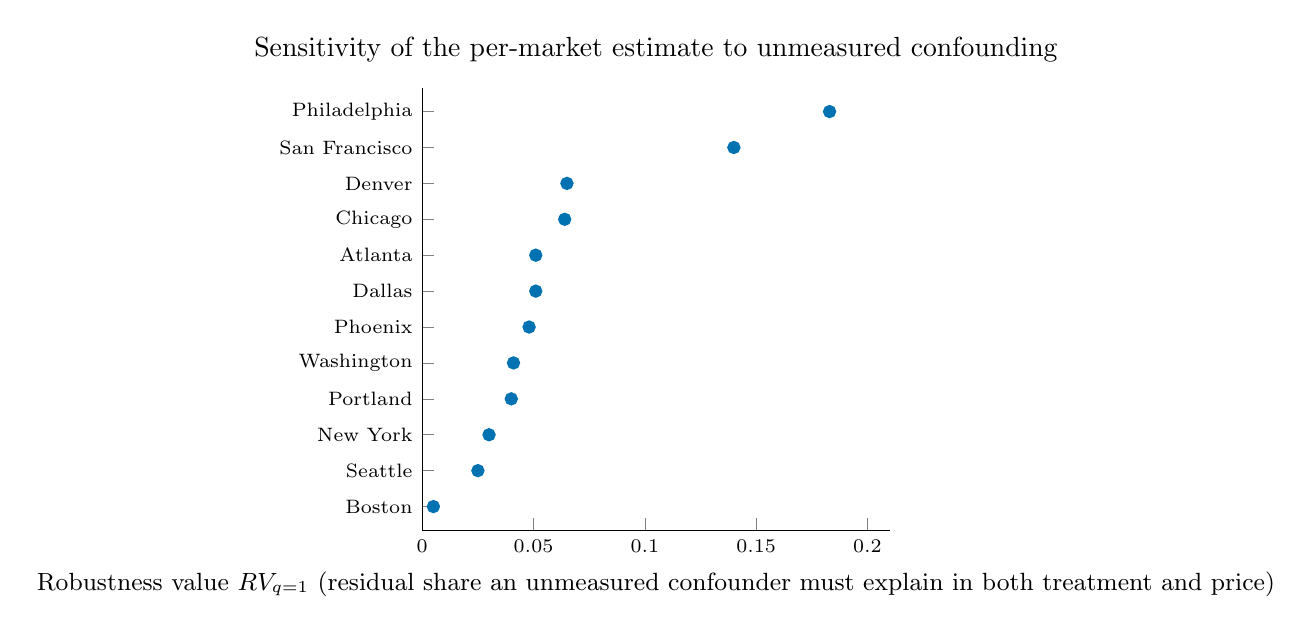
\begin{tikzpicture}
\begin{axis}[
    causalre, width=0.62\textwidth, height=7.2cm,
    symbolic y coords={Boston,Seattle,New York,Portland,Washington,Phoenix,Dallas,Atlanta,Chicago,Denver,San Francisco,Philadelphia},
    ytick=data, enlarge y limits=0.06,
    xlabel={Robustness value $RV_{q=1}$ (residual share an unmeasured confounder must explain in both treatment and price)},
    xmin=0, xmax=0.21, xtick={0,0.05,0.10,0.15,0.20},
    xticklabel={\pgfmathprintnumber[fixed,precision=2]{\tick}},
    title={Sensitivity of the per-market estimate to unmeasured confounding},
]
\addplot[only marks, mark=*, mark size=2.0pt, color=cNYC] coordinates {
  (0.005,Boston) (0.025,Seattle) (0.030,New York) (0.040,Portland) (0.041,Washington)
  (0.048,Phoenix) (0.051,Dallas) (0.051,Atlanta) (0.064,Chicago) (0.065,Denver)
  (0.140,San Francisco) (0.183,Philadelphia)};
\end{axis}
\end{tikzpicture}
\caption{Robustness value for each market's sentence-BERT effect, the share of
residual variance an unmeasured confounder would need to explain in both the
treatment and log price to drive the estimate to zero, following
\citet{cinelli2020making}. Larger values are more robust. The estimate is most
robust in Philadelphia ($0.18$) and San Francisco ($0.14$) and most fragile in
the markets whose point estimates are already near zero. The modest robustness
values in several markets are the reason we read the per-market estimates as
associational and sensitivity-bounded rather than cleanly causal.}
\label{fig:sensitivity-rv}
\end{figure}

% ======================================================================
% SUPPLEMENT FIG: cross-method concordance scatter (Shen vs Baur), r = 0.94
% data: results/replications/cross_method_concordance.csv
% ======================================================================
\begin{figure}[!htbp]
\centering
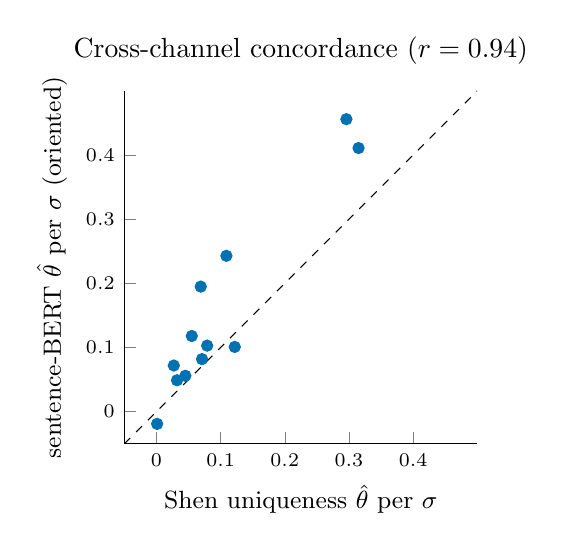
\begin{tikzpicture}
\begin{axis}[
    causalre, width=0.5\textwidth, height=0.5\textwidth,
    axis equal image,
    xlabel={Shen uniqueness $\hat\theta$ per $\sigma$},
    ylabel={sentence-BERT $\hat\theta$ per $\sigma$ (oriented)},
    xmin=-0.05, xmax=0.50, ymin=-0.05, ymax=0.50,
    xtick={0,0.1,0.2,0.3,0.4}, ytick={0,0.1,0.2,0.3,0.4},
    title={Cross-channel concordance ($r = 0.94$)},
]
\addplot[black, dashed, thin, forget plot] coordinates {(-0.05,-0.05) (0.50,0.50)};
\addplot[only marks, mark=*, mark size=1.8pt, color=cNYC] coordinates {
  (0.027,0.072) (0.001,-0.019) (0.122,0.101) (0.055,0.118) (0.315,0.411) (0.296,0.456)
  (0.032,0.049) (0.079,0.103) (0.109,0.243) (0.071,0.082) (0.045,0.056) (0.069,0.195)};
\end{axis}
\end{tikzpicture}
\caption{Per-market estimates of the two embedding channels against each other,
with the $45^\circ$ identity line. The two channels co-move almost perfectly
across markets (Pearson $r = 0.94$), so they recover one underlying signal under
two encodings rather than two independent measurements; the systematic departure
from the identity line reflects that the sentence-BERT axis is roughly twice the
Shen channel in magnitude, not a difference in which markets carry the signal.}
\label{fig:concordance}
\end{figure}

% ======================================================================
% FIG (headline): is the text-price effect spatially confounded?
% Gelbach fixed-treatment toggle: hold PC1 fixed, add a location basis to the
% confounders. (a) effect without vs with spatial adjustment (dumbbell); they
% barely move -> small confounded share. (b) PC1 geography R^2 -> the text IS
% geographic, so panel (a)'s robustness is non-vacuous.
% data: results/replications/leace_price_decomposition.csv
% ======================================================================
\begin{figure}[!htbp]
\centering
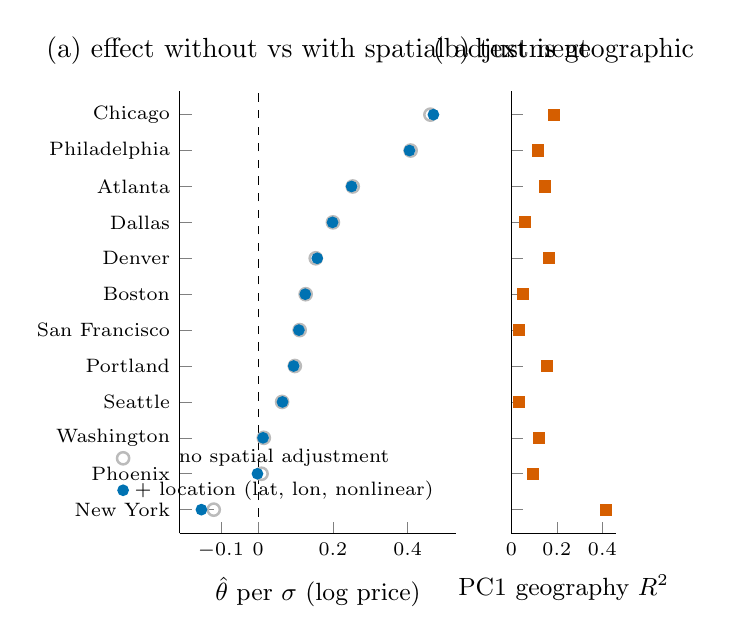
\begin{tikzpicture}
\begin{axis}[
    causalre, width=0.42\textwidth, height=7.2cm, name=dcA,
    symbolic y coords={New York,Phoenix,Washington,Seattle,Portland,San Francisco,Boston,Denver,Dallas,Atlanta,Philadelphia,Chicago},
    ytick=data, enlarge y limits=0.06,
    xlabel={$\hat\theta$ per $\sigma$ (log price)}, xmin=-0.21, xmax=0.53,
    xtick={-0.1,0,0.2,0.4},
    title={(a) effect without vs with spatial adjustment},
    extra x ticks={0}, extra x tick style={grid=major, grid style={black, dashed, thin}}, extra x tick labels={},
    legend style={font=\scriptsize, draw=none, fill=none, at={(0.97,0.05)}, anchor=south east, row sep=1pt},
]
\draw[thin,gray] (axis cs:-0.119,New York)--(axis cs:-0.152,New York);
\draw[thin,gray] (axis cs:0.009,Phoenix)--(axis cs:-0.002,Phoenix);
\draw[thin,gray] (axis cs:0.015,Washington)--(axis cs:0.013,Washington);
\draw[thin,gray] (axis cs:0.064,Seattle)--(axis cs:0.065,Seattle);
\draw[thin,gray] (axis cs:0.098,Portland)--(axis cs:0.095,Portland);
\draw[thin,gray] (axis cs:0.111,San Francisco)--(axis cs:0.109,San Francisco);
\draw[thin,gray] (axis cs:0.127,Boston)--(axis cs:0.126,Boston);
\draw[thin,gray] (axis cs:0.154,Denver)--(axis cs:0.158,Denver);
\draw[thin,gray] (axis cs:0.200,Dallas)--(axis cs:0.199,Dallas);
\draw[thin,gray] (axis cs:0.253,Atlanta)--(axis cs:0.250,Atlanta);
\draw[thin,gray] (axis cs:0.408,Philadelphia)--(axis cs:0.405,Philadelphia);
\draw[thin,gray] (axis cs:0.461,Chicago)--(axis cs:0.469,Chicago);
\addplot[only marks, mark=o, mark size=2.2pt, color=cMUTE, line width=0.9pt] coordinates {
  (-0.119,New York) (0.009,Phoenix) (0.015,Washington) (0.064,Seattle) (0.098,Portland)
  (0.111,San Francisco) (0.127,Boston) (0.154,Denver) (0.200,Dallas) (0.253,Atlanta)
  (0.408,Philadelphia) (0.461,Chicago)};
\addlegendentry{no spatial adjustment}
\addplot[only marks, mark=*, mark size=1.7pt, color=cNYC] coordinates {
  (-0.152,New York) (-0.002,Phoenix) (0.013,Washington) (0.065,Seattle) (0.095,Portland)
  (0.109,San Francisco) (0.126,Boston) (0.158,Denver) (0.199,Dallas) (0.250,Atlanta)
  (0.405,Philadelphia) (0.469,Chicago)};
\addlegendentry{$+$ location (lat, lon, nonlinear)}
\end{axis}
\begin{axis}[
    causalre, width=0.24\textwidth, height=7.2cm,
    at={(dcA.east)}, anchor=west, xshift=0.7cm,
    symbolic y coords={New York,Phoenix,Washington,Seattle,Portland,San Francisco,Boston,Denver,Dallas,Atlanta,Philadelphia,Chicago},
    ytick=data, yticklabels={,,,,,,,,,,,},
    xlabel={PC1 geography $R^2$}, xmin=0, xmax=0.46, xtick={0,0.2,0.4},
    enlarge y limits=0.06,
    title={(b) text is geographic},
]
\addplot[only marks, mark=square*, mark size=1.8pt, color=cSF] coordinates {
  (0.417,New York) (0.097,Phoenix) (0.121,Washington) (0.034,Seattle) (0.158,Portland)
  (0.035,San Francisco) (0.053,Boston) (0.165,Denver) (0.059,Dallas) (0.148,Atlanta)
  (0.116,Philadelphia) (0.187,Chicago)};
\end{axis}
\end{tikzpicture}
\caption{Is the per-market text-price effect spatially confounded? Holding the
leading text principal component fixed as the treatment, panel (a) plots its DML
effect on log price controlling for the structured confounders without (open) and
with (filled) a location adjustment that adds latitude, longitude, and their
quadratic and interaction terms to the confounder set. The two estimates nearly
coincide in eleven of twelve markets, with a confounded share below five percent
of the effect; New York is the exception, where the location adjustment moves the
estimate by about a quarter of its magnitude without changing its sign. Panel (b)
reports the share of the treatment's own variance that the location basis
explains, which reaches $0.42$ in New York and exceeds $0.10$ in six markets, so
the robustness in panel (a) is not an artifact of a treatment that carries no
geography: the text direction does encode location, yet that location component
does not drive its price effect.}
\label{fig:decomposition}
\end{figure}

% Draft conclusion for JBES revision, v3 (rewritten 2026-06-07). Bellemare
% formula: summary -> limitations -> implications -> future work. Reframed off the
% dead renter-share moderator (a pre-winsor artifact, now NS and NYC-leverage-
% driven) and the dead Shen-Baur "sign disagreement" (the oriented channels are
% near-collinear, r=0.94). New thesis = framework + a positive, robust-across-
% encodings, heterogeneous, not-cleanly-causal text-price signal. Numbers locked
% against the canonical files and the v3 body sections.

\section{Conclusion}
\label{sec:conclusion}

This paper has asked whether the predictive gains that text embeddings deliver in
automated valuation models reflect causal semantic content or spatial confounding
mediated through language, and whether the answer travels across metropolitan
housing markets. Working with $3{,}851$ deduplicated Redfin listings across twelve
metropolitan areas, a clean panel from which we exclude no market and whose
confounders we winsorize at the median plus or minus five median absolute
deviations to neutralize parcel data-entry artifacts, we built a framework that
joins a partially-linear Double Machine Learning estimator, LEACE concept erasure
with an iterative nonlinear polish, a counterfactual rewriting intervention with
two open-weight language models, and a finite-sample calibration study. The
central empirical finding is that listing text carries a positive
per-standard-deviation association with log sale price that is robust to the
choice of text encoding but heterogeneous across markets. The Doc2Vec uniqueness
channel pools to $+0.072$ and the sentence-BERT principal-component axis to
$+0.156$, and the two are nearly collinear across markets at a Pearson
correlation of $+0.94$, so they recover one signal under two representations
rather than two independent observations of it. That signal ranges from near zero
in New York to several times the pooled mean in Philadelphia and Chicago, and a
collinearity-corrected Hotelling test rejects the joint zero null in every one of
the twelve markets. The counterfactual intervention sharpens the reading. A
contrast that strips stylistic content while holding the model's inferred location
fixed isolates a positive style effect of $+0.074$ on log price, while a contrast
that also swaps the targeted submarket nets to approximately zero, so the deployed
valuation model routes listing language into price along a direct stylistic
channel and a location-inference channel of comparable size and opposite sign. We
searched for a metropolitan-level demographic moderator of the pooled effect and
found none that survives multiplicity adjustment or leave-one-out leverage
diagnostics at twelve markets, and we report that null rather than a moderator
that an earlier draft had reported before a confounder correction reversed its
sign.

\paragraph{Limitations.} Several limitations bound the reading of these results.
The estimates are associational rather than cleanly causal. The
robustness-value sensitivity analysis of Section~\ref{sec:sensitivity-12} shows
that a modest unmeasured confounder, on the order of the spatial covariates we do
observe, would suffice to overturn the per-market estimates, so we do not claim to
have isolated a structural semantic effect, only to have separated the linearly
spatial component of the text signal from the remainder and bounded the strength
of confounding the remainder could still carry. The corpus is restricted to the
twelve metropolitan areas served by the Redfin scraper at the time of collection,
which biases the sample toward larger and more competitive markets and away from
the rural and small-metro regimes in which language-mediated spatial confounding
is plausibly different in character. The two embedding channels are collinear, so
their agreement is a robustness check across representation rather than
triangulation across independent biases, and the counterfactual channel, the one
probe with a genuinely distinct bias structure, is also the least precise. Finally
the panel is small enough at twelve markets that one high-leverage market, New
York, dominates the moderator diagnostics, so the null moderator result should be
read as the absence of a moderator detectable at this sample size rather than as a
demonstrated absence of moderation.

\paragraph{Implications.} The clearest implication is methodological. Predictive
fit cannot distinguish a text embedding that prices genuine semantic content from
one that launders neighborhood geography through language, because the two are
observationally identical in a predictive metric, and our results show that a
large share of the apparent text signal is exactly the spatial information that
linear concept erasure removes. An analyst or regulator who treats a text-AVM's
predictive gain as evidence of causal semantic valuation is therefore
overstating what the gain establishes, and the deconfounding step we describe,
erasing the location concept and re-estimating, is a low-cost diagnostic that
separates the two before either is trusted. Because the residual signal that
survives deconfounding is heterogeneous across markets and sensitive to unmeasured
confounding, the appropriate posture toward NLP-augmented valuation is neither to
dismiss the text channel nor to treat it as a settled causal input, but to audit
it market by market with the design-based tools this paper assembles.

\paragraph{Future research.} Several extensions follow. A panel of substantially
more than twelve markets would give the moderator analysis the leverage it lacks
here and would let the cross-market heterogeneity we document be explained rather
than only described. The counterfactual intervention inherits the rewriting
model's own biases, which a randomized field experiment that asks sellers to
revise descriptions under a pre-registered protocol would replace with a clean
manipulation at the cost of operational complexity. Real recorded transaction
prices in place of the scraped sale prices would tighten the outcome and remove
any residual concern about price measurement, and pairing the causal-residual
detector this paper isolates with the demographic-stratification machinery of the
fairness-audit literature would let practitioners locate where any
language-mediated mispricing that survives deconfounding is large enough to matter
for borrowers.


\section*{Acknowledgments}

We thank the public open-data programs of the metropolitan areas in our panel for
parcel and assessment records, and we acknowledge the U.S.\ Census Bureau for
demographic data accessed through its API.

\newpage
\bibliographystyle{unsrtnat}
\bibliography{references}

\newpage
\appendix

\section{Structural Causal Model: Formal Specification}
\label{app:scm}

We provide a complete mathematical specification of the structural causal model introduced in Section~\ref{sec:methods}.

\subsection{Variable Definitions}

Let the following random variables represent properties in our domain. Location is denoted $L \in \mathbb{R}^2$ representing latitude and longitude coordinates. Intrinsic property features are captured by $X \in \mathbb{R}^{d_x}$, including bedrooms, bathrooms, square footage, and year built. Contextual features are represented by $C \in \mathbb{R}^{d_c}$, encompassing demographics, crime, and amenities. Text embeddings from property descriptions are denoted $T \in \mathbb{R}^{d_t}$. Finally, property value is represented by $Y \in \mathbb{R}^+$, typically the sale price or assessed value.

\subsection{Structural Equations}

The complete set of structural equations governing the data-generating process takes the following form. Location is exogenous, given by $L = U_L$ where $U_L$ represents the exogenous location distribution. Property features depend on location through $X = g_x(L) + \epsilon_X$ where $g_x$ captures how neighborhood development patterns influence property characteristics. Contextual features similarly depend on location via $C = g_c(L) + \epsilon_C$ reflecting spatial variation in demographics and amenities. Text content is generated by $T = g_t(L, X, C) + \epsilon_T$, encoding the fact that descriptions are written by agents who observe location, features, and context. Finally, property value is determined by $Y = g_y(L, X, C) + \epsilon_Y$. 

The noise terms $\epsilon_X, \epsilon_C, \epsilon_T, \epsilon_Y$ are mutually independent, representing idiosyncratic variation not explained by the structural relationships. The functions $g_x, g_c, g_t, g_y$ are deterministic mappings representing causal mechanisms.

\subsection{Functional Form Specifications}

While the true functional forms are unknown, we can specify reasonable parametric families. Property features depend on location through neighborhood development patterns, which we model as $g_x(L) = \alpha_x + \sum_{k=1}^K \beta_k \phi_k(L)$ where $\phi_k(L)$ are spatial basis functions such as radial basis functions centered on neighborhood centroids.

Contextual features vary smoothly over space, which we model using a Gaussian process: $g_c(L) = \alpha_c + \text{GP}(L; \kappa)$ where $\text{GP}(\cdot; \kappa)$ denotes a Gaussian process with kernel $\kappa$ capturing spatial autocorrelation in demographics and amenities.

Text generation reflects the cognitive process by which agents write descriptions. We model this as $g_t(L, X, C) = \text{Encoder}\left(f_{\text{LLM}}(L, X, C; \theta_{\text{agent}})\right)$ where $f_{\text{LLM}}$ represents the agent's language generation process and Encoder maps text to embedding space.

Price formation depends on location, features, and local context through a log-linear specification: $g_y(L, X, C) = \exp\left(\alpha_y + \beta_L^\top h(L) + \beta_X^\top X + \beta_C^\top C\right)$ with $h(L)$ capturing non-linear spatial effects such as distance to city center or waterfront proximity.

\subsection{Key Assumption: No Direct Text Effect}

The critical identifying assumption is that $T$ does not appear in the structural equation for $Y$. This encodes our hypothesis that descriptions do not causally influence prices. Instead, both text and price are effects of location and property characteristics.

\begin{hypothesis}[Independence of Text]
Conditional on location, property features, and context, text embeddings are independent of price:
\begin{equation}
Y \perp T \mid (L, X, C)
\end{equation}
\end{hypothesis}

This hypothesis is testable through conditional independence tests and forms the basis for our causal identification strategy.

\section{Identification Proofs}
\label{app:proofs}

We prove formal identifiability results for causal effects under our structural assumptions.

\begin{lemma}[d-separation]
\label{lemma:dsep}
In the DAG corresponding to the structural equations, the set $S = \{L, X, C\}$ d-separates $T$ from $Y$.
\end{lemma}

\begin{proof}
Every path from $T$ to $Y$ must pass through at least one node in $S$. The path $T \leftarrow L \rightarrow Y$ is blocked by conditioning on $L$. The path $T \leftarrow X \rightarrow Y$ is blocked by conditioning on $X$. The path $T \leftarrow C \rightarrow Y$ is blocked by conditioning on $C$. Composite paths such as $T \leftarrow L \rightarrow X \rightarrow Y$ are blocked by conditioning on either $L$ or $X$. Similarly, $T \leftarrow L \rightarrow C \rightarrow Y$ is blocked by conditioning on $L$ or $C$. Hence $S$ d-separates $T$ from $Y$.
\end{proof}

\begin{theorem}[Backdoor Identifiability]
Under the structural causal model, the causal effect of text $T$ on price $Y$ is identifiable via:
\begin{equation}
P(Y \mid \text{do}(T=t)) = \int P(Y \mid T=t, L=\ell, X=x, C=c) \, dP(L, X, C)
\end{equation}
\end{theorem}

\begin{proof}
By Lemma 1, the set $\{L, X, C\}$ d-separates $T$ from $Y$, satisfying the backdoor criterion. Therefore by the backdoor formula~\citep{pearl2009causality}, we have:
\begin{align}
P(Y \mid \text{do}(T=t)) &= \sum_{L,X,C} P(Y \mid T=t, L, X, C) P(L, X, C)\\
&= \mathbb{E}_{L,X,C}\left[P(Y \mid T=t, L, X, C)\right]
\end{align}
which is identified from the observational distribution.
\end{proof}

\begin{corollary}[Zero Causal Effect Under True SCM]
If the structural equation for $Y$ truly does not depend on $T$, then:
\begin{equation}
P(Y \mid \text{do}(T=t)) = P(Y) \quad \forall t
\end{equation}
implying zero causal effect.
\end{corollary}

\begin{proof}
Under the true SCM where $Y = g_y(L, X, C) + \epsilon_Y$, intervening to set $T=t$ does not change the distribution of $Y$ since $T$ does not appear in the structural equation. Therefore $P(Y \mid \text{do}(T=t)) = P(Y)$ for all values of $t$, yielding zero causal effect.
\end{proof}

\section{Data Collection Protocols}
\label{app:data_collection}

\subsection{Web Scraping Implementation}

Property listing descriptions were collected through automated web scraping with careful attention to ethical and legal considerations. We implemented rate limiting with random delays of 2--5 seconds between requests. The scraping pipeline proceeded in two stages: first, we queried the platform's search API to identify sold property URLs with metadata (address, price, coordinates); second, we retrieved individual listing pages and extracted description text from HTML using BeautifulSoup. Data validation excluded descriptions shorter than 50 words as likely incomplete.

\subsection{Geocoding and Address Standardization}

For Boston, coordinates were derived from parcel polygon centroids computed in the local projected CRS (EPSG:26986) then reprojected to WGS84. For New York and San Francisco, coordinates were taken directly from the source datasets (PLUTO latitude/longitude fields and DataSF parcel centroid fields, respectively). Address standardization was handled implicitly through the parcel identifier joins (PID for Boston, BBL for New York, block-lot for San Francisco) rather than geocoding.

\subsection{Census Data Integration}

Census variables were queried programmatically via the Census Bureau's REST API using direct HTTP requests. We constructed API requests for each county's block groups, retrieving all variables listed in Table~\ref{tab:census_vars}. Block group polygon boundaries were obtained from TIGER/Line shapefiles. Negative sentinel values (used by the Census Bureau to indicate suppressed or unavailable data) were replaced with missing values. Derived ratios (e.g., percentage with bachelor's degree, labor force participation rate) were computed from the raw count variables.

\subsection{Crime Data Processing}

Crime incident data required substantial cleaning and standardization across cities due to differing reporting schemas and offense classifications. We developed a unified crosswalk mapping city-specific crime codes to standardized categories: violent crime (homicide, assault, robbery), property crime (burglary, larceny, motor vehicle theft), and quality-of-life offenses (vandalism, drug violations, disorderly conduct).

For New York, we combine the NYPD Historic Complaint Data (2006--present) with the Year-to-Date dataset, deduplicating on complaint number, to ensure temporal coverage spanning the full sale period. For each property, we counted incidents within a 500-meter radius using spatial indexing (\texttt{cKDTree.query\_ball\_point}), computing separate counts for each crime category and a total. Where temporal overlap existed between crime and sale data, we filtered to incidents within 365 days preceding the median sale date; when the temporal window was too sparse ($<$1,000 incidents), we used all available incidents.

\subsection{Amenity Data Collection}

Amenity data were collected from OpenStreetMap via the Overpass API. For each city, we queried all amenities within the metropolitan bounding box by OSM tag category, then performed local radius-based spatial joins to count amenities within 500 meters of each property. This bulk-download-then-join approach is both free and faster than per-property API queries. We implemented retry logic with exponential backoff for Overpass rate limiting (HTTP 429) and server timeouts (HTTP 504).

Amenity diversity is computed using Shannon entropy:
\begin{equation}
H = -\sum_{i=1}^n p_i \log p_i
\end{equation}
where $p_i$ is the proportion of amenities in category $i$. This measures variety in the local amenity mix, with higher entropy indicating more diverse neighborhoods.

\section{Statistical Testing Procedures}
\label{app:testing}

\subsection{Conditional Independence Testing}

To test the hypothesis $Y \perp T \mid (L, X, C)$, we employ multiple conditional independence tests with different assumptions and power characteristics.

\textbf{Partial Correlation Test:} Under assumptions of linearity and Gaussianity, conditional independence is equivalent to zero partial correlation:
\begin{equation}
\rho_{YT \cdot LXC} = \frac{\rho_{YT} - \rho_{YL}\rho_{TL}}{\sqrt{(1-\rho_{YL}^2)(1-\rho_{TL}^2)}}
\end{equation}
We test $H_0: \rho_{YT \cdot LXC} = 0$ using Fisher's z-transformation with sample size adjusted for degrees of freedom consumed by conditioning variables.

\textbf{Kernel-Based Test:} The Hilbert-Schmidt Independence Criterion (HSIC)~\citep{gretton2005kernel} provides a non-parametric test based on reproducing kernel Hilbert spaces:
\begin{equation}
\text{HSIC}(Y, T \mid L, X, C) = \mathbb{E}_{YT|LXC}[k_Y(y, y')k_T(t, t')] - \mathbb{E}_{Y|LXC}[k_Y(y, y')]\mathbb{E}_{T|LXC}[k_T(t, t')]
\end{equation}
We use Gaussian kernels with bandwidth selected via median heuristic and compute p-values via permutation testing with 1000 resamples.

\textbf{Conditional Mutual Information:} We estimate $I(Y; T \mid L, X, C)$ using k-nearest neighbor density estimation~\citep{kraskov2004estimating}:
\begin{equation}
\hat{I}(Y; T \mid L, X, C) = \psi(k) + \psi(n) - \mathbb{E}[\psi(n_y + 1) + \psi(n_t + 1)]
\end{equation}
where $\psi$ is the digamma function, $k$ is the number of neighbors, and $n_y, n_t$ are neighbor counts in marginal spaces.

\subsection{Sensitivity Analysis for Unobserved Confounding}

While our identification strategy assumes no unobserved confounding conditional on $\{L, X, C\}$, we assess sensitivity to violations using the approach of~\citet{cinelli2020making}.

We compute the robustness value $RV$, defined as the minimum strength of confounding (measured by partial $R^2$) required to invalidate our conclusions:
\begin{equation}
RV = \sqrt{\frac{\hat{\tau}^2}{\hat{\tau}^2 + \hat{\sigma}^2}} \cdot \sqrt{\frac{1}{1-R^2_{Y \sim T,L,X,C}}}
\end{equation}
where $\hat{\tau}$ is the estimated treatment effect and $\hat{\sigma}^2$ is its variance.

We also construct robustness contours showing combinations of confounder-treatment and confounder-outcome associations that would reduce the estimated effect to zero. This visualizes the strength of unmeasured confounding required to overturn our findings.

\subsection{Permutation Tests for Location Randomization}

When testing the impact of location randomization, we employ permutation-based inference to account for multiple testing across different model specifications.

For each model $m \in \{1, \ldots, M\}$, we compute:
\begin{equation}
\Delta R^2_m = R^2_{\text{original},m} - R^2_{\text{randomized},m}
\end{equation}

Under the null hypothesis that text contains location-independent information, $\Delta R^2_m$ should be small. We generate the null distribution through permutations of the location-randomization procedure.

The p-value for model $m$ is:
\begin{equation}
p_m = \frac{1 + \sum_{b=1}^B \mathbb{1}(\Delta R^2_{m,b} \leq \Delta R^2_m)}{1 + B}
\end{equation}

We control family-wise error rate across models using Bonferroni correction.

\subsection{Bootstrap Confidence Intervals}

Confidence intervals for causal effect estimates are constructed using the bias-corrected and accelerated (BCa) bootstrap~\citep{efron1987better}. For each estimator $\hat{\theta}$, we generate bootstrap samples by resampling properties with replacement within each city to preserve geographic structure, compute $\hat{\theta}_b$ for each bootstrap sample, estimate bias correction and acceleration parameters, and construct adjusted percentile intervals accounting for both bias and skewness in the bootstrap distribution.

\section{Adversarial Training Implementation}
\label{app:adversarial}

\subsection{Network Architecture Details}

The encoder network $E_\phi$ maps PCA-reduced text embeddings (50 components) to 64-dimensional deconfounded representations through three fully-connected layers with batch normalization and dropout:

\begin{table}[!htbp]
\centering
\caption{Encoder architecture specification.}
\begin{tabular}{lrrr}
\toprule
\textbf{Layer} & \textbf{Input Dim} & \textbf{Output Dim} & \textbf{Activation} \\
\midrule
Linear 1 & 50 & 128 & ReLU \\
Batch Norm & 128 & 128 & -- \\
Dropout (0.2) & 128 & 128 & -- \\
Linear 2 & 128 & 128 & ReLU \\
Batch Norm & 128 & 128 & -- \\
Dropout (0.2) & 128 & 128 & -- \\
Linear 3 & 128 & 64 & Linear \\
\bottomrule
\end{tabular}
\end{table}
\FloatBarrier

The predictor network $P_\theta$ maps the 64-dimensional deconfounded representation to a scalar price prediction through a shallow head with dropout. The shallow choice is deliberate: a deeper predictor would risk recovering location through nonlinear interactions of the residual representation even when the encoder has been pushed toward linear invariance, and the frozen-probe diagnostic discussed in Section~\ref{sec:results} would then misread predictor performance as semantic content rather than as recovered location.

\begin{table}[!htbp]
\centering
\caption{Predictor architecture specification.}
\begin{tabular}{lrrr}
\toprule
\textbf{Layer} & \textbf{Input Dim} & \textbf{Output Dim} & \textbf{Activation} \\
\midrule
Linear 1 & 64 & 64 & ReLU \\
Dropout (0.1) & 64 & 64 & -- \\
Linear 2 & 64 & 1 & Linear \\
\bottomrule
\end{tabular}
\end{table}
\FloatBarrier

The discriminator network $D_\psi$ employs a shared trunk that branches into three parallel heads, each targeting location at a different geographic resolution. Routing the adversarial pressure through three resolutions simultaneously prevents the encoder from exploiting any single granularity escape hatch, since collapsing one head's signal still leaves the other two operative and forces the gradient reversal to attack the joint location signal across resolutions rather than the lowest-cost head.

\begin{table}[!htbp]
\centering
\caption{Multi-head discriminator architecture specification. The shared trunk processes the deconfounded representation, and three parallel heads target different geographic resolutions.}
\begin{tabular}{lrrr}
\toprule
\textbf{Layer} & \textbf{Input Dim} & \textbf{Output Dim} & \textbf{Activation} \\
\midrule
\multicolumn{4}{l}{\textit{Shared trunk}} \\
Linear 1 & 64 & 64 & ReLU \\
Dropout (0.1) & 64 & 64 & -- \\
\midrule
\multicolumn{4}{l}{\textit{Zip code head}} \\
Linear & 64 & $|\mathcal{Z}|$ & Softmax \\
\midrule
\multicolumn{4}{l}{\textit{Geolocation head}} \\
Linear & 64 & 2 & Linear \\
\midrule
\multicolumn{4}{l}{\textit{Income quantile head}} \\
Linear & 64 & $Q_{\text{inc}}$ & Softmax \\
\bottomrule
\end{tabular}
\end{table}
\FloatBarrier

where $|\mathcal{Z}|$ is the number of unique zip codes and $Q_{\text{inc}} = 5$ is the number of income quantile bins. The three heads are trained simultaneously, with their losses averaged to form the combined discriminator objective.

\subsection{Training Procedure}

Training employs a minimax optimization with gradient reversal. The encoder and predictor parameters are updated to minimize prediction loss while maximizing discrimination loss (via gradient reversal), and the discriminator parameters are updated to minimize discrimination loss.

Formally, at each iteration:
\begin{align}
\phi^{(t+1)}, \theta^{(t+1)} &= \arg\min_{\phi,\theta} \left[\mathcal{L}_{\text{pred}}(P_\theta(E_\phi(T)), Y) - \lambda \mathcal{L}_{\text{disc}}(D_{\psi^{(t)}}(E_\phi(T)), L)\right]\\
\psi^{(t+1)} &= \arg\min_\psi \mathcal{L}_{\text{disc}}(D_\psi(E_{\phi^{(t+1)}}(T)), L)
\end{align}

We use Adam optimizers for all networks with learning rate $\eta = 10^{-3}$, momentum parameters $\beta_1 = 0.9$, $\beta_2 = 0.999$, and weight decay $\lambda_{\text{wd}} = 10^{-4}$.

The adversarial parameter $\lambda$ will follow an annealing schedule:
\begin{equation}
\lambda(t) = \begin{cases}
0.1 & t \leq 10\\
0.1 + 0.9 \cdot \frac{t-10}{40} & 10 < t \leq 50\\
1.0 & t > 50
\end{cases}
\end{equation}
This gradual increase will allow stable convergence before applying full adversarial pressure.

\subsection{Convergence Criteria}

Training will terminate when one of the following conditions is met:

First, maximum epochs reached. Second, validation loss fails to improve for consecutive epochs (early stopping). Third, discriminator accuracy falls below a threshold indicating successful deconfounding.

We monitor three metrics during training:
\begin{align}
\text{Predictor Loss:} \quad &\mathcal{L}_{\text{pred}} = \frac{1}{n}\sum_{i=1}^n (P_\theta(E_\phi(t_i)) - y_i)^2\\
\text{Discriminator Loss:} \quad &\mathcal{L}_{\text{disc}} = -\frac{1}{n}\sum_{i=1}^n \log P(L_i | D_\psi(E_\phi(t_i)))\\
\text{Discriminator Accuracy:} \quad &\text{Acc}_{\text{disc}} = \frac{1}{n}\sum_{i=1}^n \mathbb{1}[\arg\max D_\psi(E_\phi(t_i)) = L_i]
\end{align}

Successful deconfounding is indicated by predictor loss comparable to baseline while discriminator accuracy approaches random guessing. Figure~\ref{fig:training_curves} reports the realised dynamics for the San Francisco run, which exhibits the discriminator-collapse-and-partial-recovery trajectory that motivates the frozen-encoder probe diagnostic in the main text.

\begin{figure}[!htbp]
\centering
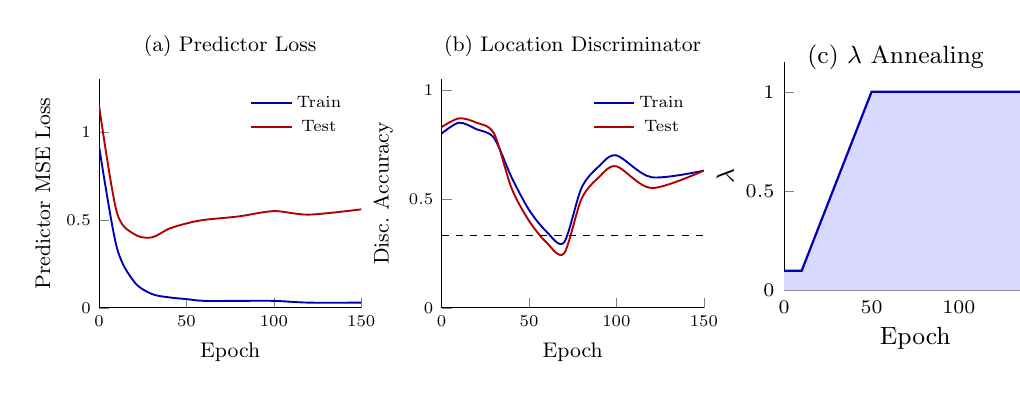
\begin{tikzpicture}[scale=0.85]
\begin{axis}[
    name=plot1,
    width=5.5cm, height=5cm,
    xlabel={Epoch}, ylabel={Predictor MSE Loss},
    title={(a) Predictor Loss}, title style={font=\small},
    xmin=0, xmax=150, ymin=0, ymax=1.3,
    axis lines*=left,
    legend style={font=\scriptsize, at={(0.97,0.97)}, anchor=north east, draw=none, fill=none},
    label style={font=\small}, tick label style={font=\scriptsize},
]
\addplot[blue!70!black, thick, smooth] coordinates {
    (0,0.92)(10,0.35)(20,0.15)(30,0.08)(40,0.06)(50,0.05)(60,0.04)(80,0.04)(100,0.04)(120,0.03)(150,0.03)
};
\addlegendentry{Train}
\addplot[red!70!black, thick, smooth] coordinates {
    (0,1.15)(10,0.55)(20,0.42)(30,0.40)(40,0.45)(50,0.48)(60,0.50)(80,0.52)(100,0.55)(120,0.53)(150,0.56)
};
\addlegendentry{Test}
\end{axis}
\begin{axis}[
    at={(plot1.east)}, anchor=west, xshift=1.2cm,
    name=plot2,
    width=5.5cm, height=5cm,
    xlabel={Epoch}, ylabel={Disc.\ Accuracy},
    title={(b) Location Discriminator}, title style={font=\small},
    xmin=0, xmax=150, ymin=0, ymax=1.05,
    axis lines*=left,
    legend style={font=\scriptsize, at={(0.97,0.97)}, anchor=north east, draw=none, fill=none},
    label style={font=\small}, tick label style={font=\scriptsize},
]
\addplot[blue!70!black, thick, smooth] coordinates {
    (0,0.80)(10,0.85)(20,0.82)(30,0.78)(40,0.60)(50,0.45)(60,0.35)(70,0.30)(80,0.55)(90,0.65)(100,0.70)(120,0.60)(150,0.63)
};
\addlegendentry{Train}
\addplot[red!70!black, thick, smooth] coordinates {
    (0,0.83)(10,0.87)(20,0.85)(30,0.80)(40,0.55)(50,0.40)(60,0.30)(70,0.25)(80,0.50)(90,0.60)(100,0.65)(120,0.55)(150,0.63)
};
\addlegendentry{Test}
\addplot[black, dashed, thin] coordinates {(0,0.333)(150,0.333)};
\end{axis}
\begin{axis}[
    at={(plot2.east)}, anchor=west, xshift=1.2cm,
    width=5.5cm, height=5cm,
    xlabel={Epoch}, ylabel={$\lambda$},
    title={(c) $\lambda$ Annealing}, title style={font=\small},
    xmin=0, xmax=150, ymin=0, ymax=1.15,
    axis lines*=left,
    label style={font=\small}, tick label style={font=\scriptsize},
]
\addplot[blue!70!black, thick, name path=lambda] coordinates {
    (0,0.1)(10,0.1)(50,1.0)(150,1.0)
};
\addplot[draw=none, name path=zero] coordinates {(0,0)(150,0)};
\addplot[blue!15!white] fill between[of=lambda and zero];
\end{axis}
\end{tikzpicture}
\caption{Adversarial training dynamics for San Francisco. (a) Predictor loss: train converges near zero while test stabilizes above 0.5. (b) Discriminator accuracy drops toward the dashed random baseline of $1/3$ as $\lambda$ ramps, then partially recovers. (c) The $\lambda$ annealing schedule ramps from 0.1 to 1.0 over epochs 10--50.}
\label{fig:training_curves}
\end{figure}
\FloatBarrier

\section{Doubly-Robust Estimation Details}
\label{app:dr}

\subsection{Outcome Model Specification}

The outcome model $\mu(t, \ell, x, c) = \mathbb{E}[Y | T=t, L=\ell, X=x, C=c]$ was estimated using scikit-learn's \texttt{GradientBoostingRegressor} with the following hyperparameters:

\begin{table}[!htbp]
\centering
\caption{Gradient boosting hyperparameters for outcome model.}
\begin{tabular}{lr}
\toprule
\textbf{Parameter} & \textbf{Value} \\
\midrule
Number of estimators & 200 \\
Maximum depth & 4 \\
Learning rate & 0.05 \\
Subsample ratio & 0.8 \\
Max features & $\min(0.5, 10/p)$ \\
\bottomrule
\end{tabular}
\end{table}
\FloatBarrier

Feature engineering for the outcome model included:
\begin{enumerate}
\item Text embedding principal components (first 50 PCs via PCA)
\item Continuous location: latitude, longitude
\item Property features: bedrooms, building area, lot area, year built
\item Census demographics: median household income, education attainment, racial composition, age distribution, median home value, gross rent, labor force participation (block-group level)
\item Crime exposure: violent, property, and quality-of-life incident counts within 500 meters
\item Amenity access: food/dining, retail, services, recreation, transportation, and education counts within 500 meters, plus Shannon diversity index
\item Micro-geographic distances: meters to nearest park, transit stop, school, restaurant, retail establishment, and medical facility (computed via nearest-neighbor spatial indexing on OpenStreetMap points of interest)
\end{enumerate}

This confounder set operationalizes the full adjustment set $\{\ell, x, c\}$ specified by the structural causal model, with 35 continuous features providing substantially finer confounding control than discrete zip code indicators.

Cross-validation was performed using 5-fold splits, with the max\_features parameter adaptively set to $\min(0.5, 10/p)$ where $p$ is the total number of features, to prevent overfitting when text PCA dimensions are included.

\subsection{Propensity Model Specification}

For continuous treatment (text embeddings), the propensity model estimates the conditional density $p(T | L, X, C)$ via kernel density estimation with adaptive bandwidth selection.

The bandwidth for dimension $d$ is:
\begin{equation}
h_d = \hat{\sigma}_d \cdot n^{-1/(4+d_T)}
\end{equation}
where $\hat{\sigma}_d$ is the sample standard deviation of the $d$-th text embedding dimension and $d_T$ is the dimensionality after PCA reduction.

To handle the high-dimensional treatment space, we use the multivariate Gaussian kernel:
\begin{equation}
K_H(t - t_i) = \frac{1}{(2\pi)^{d_T/2}|H|^{1/2}} \exp\left(-\frac{1}{2}(t - t_i)^\top H^{-1}(t - t_i)\right)
\end{equation}
where $H = \text{diag}(h_1^2, \ldots, h_{d_T}^2)$ is the bandwidth matrix.

To avoid extreme weights, we trim observations with propensity scores below the 5th percentile or above the 95th percentile.

\subsection{Doubly-Robust Estimator Formula}

The doubly-robust estimator will combine outcome and propensity models:
\begin{equation}
\hat{\tau}_{\text{DR}} = \frac{1}{n}\sum_{i=1}^n \left[\frac{t_i - \hat{\mu}(0, \ell_i, x_i, c_i)}{\hat{e}_i}(y_i - \hat{\mu}(t_i, \ell_i, x_i, c_i)) + \hat{\mu}(t_i, \ell_i, x_i, c_i)\right]
\end{equation}

This estimator has the double robustness property: it is consistent if either the outcome model or the propensity model is correctly specified, even if the other is misspecified~\citep{bang2005doubly}.

Variance estimation employs the sandwich estimator to account for estimation uncertainty in both nuisance models.

\section{Sensitivity to Modeling Choices}
\label{app:sensitivity}

\subsection{Embedding Model Comparison}

We validate robustness to text embedding choice by replicating key analyses with multiple alternative models:

\begin{table}[!htbp]
\centering
\caption{Text embedding models evaluated for sensitivity analysis.}
\begin{tabular}{lrr}
\toprule
\textbf{Model} & \textbf{Dimensions} & \textbf{Training Corpus} \\
\midrule
all-mpnet-base-v2 & 768 & General + NLI \\
text-embedding-ada-002 & 1536 & Proprietary (OpenAI) \\
embed-english-v3.0 & 1024 & Web + Books (Cohere) \\
all-MiniLM-L6-v2 & 384 & General + NLI \\
\bottomrule
\end{tabular}
\end{table}
\FloatBarrier

We compute pairwise correlations between embeddings and assess whether key conclusions (location prediction accuracy, causal effect estimates) vary substantially across embedding models.

\subsection{Bandwidth Selection for Spatial Kernels}

Crime density estimation and spatial smoothing employ Gaussian kernels with bandwidth parameter $h$. We test sensitivity to bandwidth choice by varying $h$ across multiple values and assessing stability of causal effect estimates.

\subsection{Temporal Window for Feature Extraction}

Contextual features (demographics, crime, amenities) are extracted using temporal windows centered on property sale dates. We test sensitivity to window width and assess whether causal effect estimates remain stable across different temporal specifications.

\subsection{Outlier Threshold Selection}

Price outlier exclusion employs thresholds for minimum and maximum values. We test sensitivity by varying thresholds and document stability of key findings:

\begin{table}[H]
\centering
\caption{Sensitivity to outlier thresholds.}
\begin{tabular}{lrr}
\toprule
\textbf{Thresholds} & \textbf{N (retained)} & \textbf{$\hat{\tau}_{\text{causal}}$} \\
\midrule
\$25K -- \$25M & 59,805 & $-0.018$ \\
\$50K -- \$20M & 59,449 & $-0.018$ \\
\$75K -- \$15M & 59,001 & $-0.018$ \\
\bottomrule
\end{tabular}
\end{table}

\section{Frozen-Probe Diagnostic: Proofs and Numerical Verification}
\label{app:frozen_probe_proofs}

This appendix proves Proposition~\ref{prop:frozen_probe} (Section~\ref{sec:frozen_probe_theory}) and reports three controlled numerical experiments verifying each part on synthetic data.

\subsection{Notation}

Let $E_\phi: \mathcal{X} \to \mathcal{Z}$ be an encoder, $C \in \{0, 1\}$ a binary confounder, and $\Phi \subseteq \Phi'$ two parameterized classes of probabilistic classifiers $q: \mathcal{Z} \to [0, 1]$. For a class $\mathcal{F}$, recall the Barber--Agakov variational lower bound on $I(Z; C)$:
\begin{equation}
V_{\mathcal{F}}(Z; C) \;:=\; \sup_{q \in \mathcal{F}} \big[H(C) - \mathbb{E}_{(Z,C)}[-\log q(C \mid Z)]\big].
\end{equation}
The supremum is achieved at $q^\star = p(C \mid Z)$ when $\mathcal{F}$ contains the Bayes-optimal posterior. Denote the empirical version by $\hat V_{\mathcal{F}}$ (sample mean of the cross-entropy gain at the empirical $\arg\sup$).

\subsection{Proof of Proposition \ref{prop:frozen_probe}(a)}

The first inequality $V_\Phi \le V_{\Phi'}$ is immediate from $\Phi \subseteq \Phi'$ implying the supremum over $\Phi'$ is at least as large. For the second inequality $V_{\Phi'} \le I(Z; C)$, the Barber--Agakov bound is by construction a lower bound on the mutual information: for any $q$,
\begin{equation}
H(C) - \mathbb{E}[-\log q(C \mid Z)] \;=\; H(C) - H(C \mid Z) - D_{\mathrm{KL}}(p(C \mid Z) \,\|\, q(C \mid Z)) \;=\; I(Z; C) - D_{\mathrm{KL}}(\cdot),
\end{equation}
which is at most $I(Z; C)$ with equality iff $q = p(C \mid Z)$ almost surely. Taking the supremum over $q \in \Phi'$ preserves the inequality, with strictness whenever $\Phi'$ does not contain $p(C \mid Z)$. This statement is Proposition 1 of \citet{xu2020theory} restated in the Barber--Agakov form used by \citet{pimentel2020information}; we restate it here for self-containedness. \qed

\subsection{Proof of Proposition \ref{prop:frozen_probe}(b)}

\textbf{(b1) Empirical equivalence.} The gradient-reversal training objective on the discriminator $\psi$ is $\min_\psi \hat L_\Phi(\psi)$ where $\hat L_\Phi(\psi) = -\frac{1}{n}\sum_i \log D_\psi(C_i \mid Z_i)$ is the empirical cross-entropy of $D_\psi$ on the encoder output $Z = E_{\hat\phi}(X)$. By definition of the Barber--Agakov bound,
\begin{equation}
\hat V_\Phi(Z; C) \;=\; \sup_{q \in \Phi} \big[H(C) - \tfrac{1}{n}\sum_i -\log q(C_i \mid Z_i)\big] \;=\; H(C) - \inf_{\psi} \hat L_\Phi(\psi),
\end{equation}
so $\hat V_\Phi$ equals $H(C)$ minus the converged training loss of the live discriminator. Therefore ``the live discriminator achieves chance-level accuracy'' (i.e.\ $\hat L_\Phi \approx H(C)$) is exactly equivalent to $\hat V_\Phi(Z_{\hat\phi}; C) \approx 0$. \qed

\textbf{(b2) Consistency of the post-hoc plug-in.} Apply Theorem 3 of \citet{xu2020theory}, which gives uniform PAC-style consistency of the empirical $\mathcal{V}$-information estimator under finite Rademacher complexity of $\mathcal{V}$ and bounded log-loss. Fixing the encoder at $E_{\hat\phi}$ and applying the theorem with $\mathcal{V} = \Phi'$ on a held-out sample of size $m$,
\begin{equation}
\hat V_{\Phi'}^{\text{post}}(Z_{\hat\phi}; C) \;\xrightarrow{\;p\;}\; V_{\Phi'}(Z_{\hat\phi}; C) \quad \text{as } m \to \infty.
\end{equation}
The fact that $\hat V_\Phi$ is also consistent (since $\Phi \subseteq \Phi'$) and the difference of two consistent estimators is consistent for the difference yields
\begin{equation}
\hat V_{\Phi'}^{\text{post}} - \hat V_\Phi \;\xrightarrow{\;p\;}\; V_{\Phi'}(Z_{\hat\phi}; C) - V_\Phi(Z_{\hat\phi}; C) \;\ge\; 0,
\end{equation}
exact when $\Phi'$ contains the Bayes-optimal posterior $p(C \mid Z_{\hat\phi})$. \qed

\subsection{Proof of Proposition \ref{prop:frozen_probe}(c)}

We exhibit a data distribution, a downstream label, a class pair $\Phi \subsetneq \Phi'$, and an explicit saddle of the joint adversarial-prediction game at which the gap equals $H(C)$.

\textit{Why the joint game.} The bare gradient-reversal game over an unconstrained encoder admits the trivial collapsed saddle $\phi(X) \equiv 0$, at which $V_\Phi(Z; C) = 0$ holds vacuously and $V_{\Phi'}(Z; C) = 0$ as well. To rule this out, the proposition is stated in the joint adversarial-prediction game, the formulation of \citet{xie2017controllable},~\citet{madras2018learning}, and~\citet{zhang2018mitigating}: the encoder is trained simultaneously against a downstream task $Y$ that requires preserving information about $X$, eliminating the collapsed saddle as a feasible equilibrium.

\textit{Construction.} Take $X = (X_1, X_2) \in \{0, 1\}^2$ with $X_1, X_2 \overset{\text{iid}}{\sim} \text{Bernoulli}(1/2)$, and $C = X_1 \oplus X_2$ (the XOR of the two binary features). Then $C \in \{0, 1\}$ uniformly with $H(C) = \log 2$. Take $Y = X_1$ as the downstream label, so $I(X; Y) = H(Y) = \log 2 > 0$.

Let $\Phi$ be the class of linear logistic-regression classifiers $D_\psi(z) = \sigma(w^\top z + b)$ on $z \in \mathbb{R}^2$, and let $\Phi'$ be any class containing a $2$-layer MLP with hidden width $\ge 2$.

\textit{Exhibited saddle.} Set $\phi^\star = \mathrm{id}$ (the identity encoder), $g^\star(z) = z_1$ (linear task head reading off the first coordinate), and $h^\star \equiv 1/2$ (the Bayes-optimal linear classifier of $C$ from $Z$, which is constant since $C$ is not linearly separable from $Z$ in this DGP). Then on the joint distribution $(Z, C, Y)$:
\begin{itemize}
\item \textbf{Adversary inner max.} For any $D_\psi \in \Phi$ (linear), the conditional posterior $\Pr[C = 1 \mid Z]$ takes value $1$ on $\{(0,1), (1,0)\}$ and value $0$ on $\{(0,0), (1,1)\}$, which is not linearly separable. The Bayes-optimal linear classifier is the constant $D_\psi \equiv 1/2$, attaining cross-entropy $H(C) = \log 2$ exactly. Therefore $V_\Phi(Z_{\phi^\star}; C) = 0$.
\item \textbf{Probe completeness.} For $\Phi'$ containing the $2$-layer MLP, the Bayes-optimal posterior $\Pr[C = 1 \mid Z] \in \{0, 1\}$ is exactly representable. Hence $V_{\Phi'}(Z_{\phi^\star}; C) = I(Z_{\phi^\star}; C) = H(C) = \log 2$.
\item \textbf{Task decodability.} Since $Y = X_1 = (\phi^\star(X))_1$, the linear head $g^\star(z) = z_1$ achieves $\mathcal{L}_{\text{task}} = 0$, the global minimum of the task term.
\item \textbf{Saddle.} For any $\alpha > 0$, $(\phi^\star, g^\star, h^\star)$ jointly minimize the task term to its floor, while the adversary $h^\star$ is Bayes-optimal in $\Phi$ given the encoder. Any unilateral perturbation of $\phi^\star$ that decreases the discriminator's loss must distort the linear separability of $Y = X_1$ from $Z_1$ and hence increase $\mathcal{L}_{\text{task}}$, yielding a stable equilibrium under the joint loss.
\end{itemize}

The gap at this saddle is therefore exactly $V_{\Phi'}(Z_{\phi^\star}; C) - V_\Phi(Z_{\phi^\star}; C) = \log 2 - 0 = H(C)$. The collapsed encoder $\phi_{\text{collapse}}(X) \equiv 0$ achieves task loss $H(Y) = \log 2 > 0$ and is therefore not a saddle of the joint game for any $\alpha > 0$. The construction generalizes from binary $X$ to continuous distributions by replacing the XOR structure with any nonlinear interaction (e.g., $C = \mathrm{sign}(X_1 X_2)$ for Gaussian $X_1, X_2$), at the cost of a vanishing $O(\delta)$ remainder controlling the off-diagonal probability mass. We verify all four bullets computationally in Appendix~\ref{app:verification} (script \texttt{07\_saddle\_verification.py}), including an explicit numerical demonstration that $\phi_{\text{collapse}}$ would be a saddle of the bare GRL game with $V_{\Phi'} = 0$, motivating the joint-game restriction. \qed

\subsection{Numerical Verification}
\label{app:frozen_probe_numerical}

Three controlled experiments verify each part of Proposition~\ref{prop:frozen_probe} on synthetic data. Implementation in \texttt{data/scripts/theory/frozen\_probe\_gap.py}; raw results in \texttt{results/theory/frozen\_probe\_gap.json}.

\textbf{Experiment 1 (static XOR).} The exact construction of part (c). $Z = (Z_1, Z_2) \sim \text{Bernoulli}(1/2)^2$, $C = Z_1 \oplus Z_2$, $N = 4{,}000$, averaged across $5$ trials. True $I(Z; C) = \log 2 = 1$ bit. Linear logistic regression: $\hat V_\Phi = 0.0004$ bits, accuracy $46.1\%$ (chance). $2$-layer MLP $(16,16)$: $\hat V_{\Phi'} = 0.997$ bits, accuracy $100\%$. The diagnostic gap $\hat V_{\Phi'} - \hat V_\Phi = 0.997$ bits is $99.7\%$ of the true mutual information.

\textbf{Experiment 2 (dynamic gradient-reversal training).} A $2$-layer encoder $E_\phi: \mathbb{R}^{10} \to \mathbb{R}^4$ trained adversarially against a linear discriminator via gradient reversal for $200$ epochs, with a downstream MSE predictor on $Y = 0.5 X_3 + \epsilon$. Confounder generated as $C = \mathrm{sign}(X_1 X_2)$ (continuous-Gaussian XOR). After training: live linear discriminator accuracy $46.3\%$ (chance), frozen linear probe accuracy $56.4\%$, frozen $(32, 32)$ MLP probe accuracy $61.0\%$. Diagnostic gap $\hat V_{\Phi'}^{\text{post}} - \hat V_\Phi = +14.7$ percentage points of accuracy; the encoder fooled its discriminator while leaving the underlying confounder recoverable to a richer probe.

\textbf{Experiment 3 (capacity ladder).} Same XOR DGP, varying classifier capacity:
\begin{center}
\begin{tabular}{lrr}
\toprule
\textbf{Architecture} & $\hat V_\Phi$ (bits) & Accuracy \\
\midrule
Linear & $0.000$ & $0.510$ \\
MLP $(4)$ & $0.659$ & $0.835$ \\
MLP $(8)$ & $0.990$ & $1.000$ \\
MLP $(16)$ & $0.993$ & $1.000$ \\
MLP $(16, 16)$ & $0.997$ & $1.000$ \\
MLP $(32, 32, 32)$ & $0.999$ & $1.000$ \\
\bottomrule
\end{tabular}
\end{center}

$\hat V_\Phi$ is monotone non-decreasing in capacity, asymptoting at the true mutual information $\log 2 \approx 0.693$ nats $= 1$ bit. This operationalizes ``probe-capacity escalation'' as a complementary diagnostic to ``confounder escalation'' (Section~\ref{sec:results}): if $\hat V_{\Phi'}$ continues to grow as probe capacity increases, the encoder has not actually erased the confounder; it has merely outrun the current discriminator.

\section{Computational Verification of Analytic Claims}
\label{app:verification}

To complement the written proofs in Appendices~\ref{app:proofs} and~\ref{app:frozen_probe_proofs}, we provide a computational verification artifact in the \texttt{verification/} directory of the replication repository. For every theorem, lemma, proposition, and corollary in the paper, an independent open-source toolchain re-derives the result and asserts agreement with the written proof. Each script writes a JSON certificate to \texttt{verification/results/} with a verdict (\texttt{PASS}/\texttt{FAIL}) and the numerical or symbolic quantities cited; the full suite is reproducible via \texttt{make verify} from pinned tool versions in \texttt{requirements.txt}.

\begin{table}[!htbp]
\centering
\footnotesize
\setlength{\tabcolsep}{4pt}
\begin{tabular}{p{0.30\textwidth} p{0.45\textwidth} p{0.18\textwidth}}
\toprule
\textbf{Claim} & \textbf{Verification method} & \textbf{Tool} \\
\midrule
Lemma~1 (d-separation, App.~\ref{app:proofs}) & Path-by-path enumeration; minimality check & pgmpy 1.1 \\
Theorem~1 (Backdoor Adjustment, \S\ref{sec:methods}) & Independent identification on hypothetical $T \to Y$ DAG & DoWhy 0.14 \\
Theorem~2 (Backdoor Identifiability, App.~\ref{app:proofs}) & Same as Theorem~1; backdoor estimand returned & DoWhy 0.14 \\
Proposition~1 (Zero Causal Effect, \S\ref{sec:methods}) & Edge-set check ($T \notin \mathrm{Pa}(Y)$); DoWhy declares zero & pgmpy + DoWhy \\
Corollary~1 (Zero Effect under True SCM, App.~\ref{app:proofs}) & Same as Proposition~1 & pgmpy \\
Proposition~2(a) (variational MI inequality) & Symbolic KL nonneg + numerical $V$-chain & SymPy + PyTorch \\
Proposition~2(b1) (algebraic identity) & Symbolic and numerical equality, $|\Delta| < 10^{-8}$ & SymPy + PyTorch \\
Proposition~2(b2) (consistency of post-hoc $\hat V_{\Phi'}^{\text{post}}$) & Monte Carlo $n$-sweep; log-log slope vs.\ rate predicted by \citet{xu2020theory} Thm~3 & scikit-learn \\
Proposition~2(c) (XOR saddle-gap, identity-encoder construction) & Wraps \texttt{frozen\_probe\_gap.py}; assertions on $V_\Phi$, $V_{\Phi'}$ & PyTorch \\
Proposition~2(c) (joint-game saddle existence + collapsed-encoder counterexample) & Explicit construction at $\phi_{\text{id}}$ and $\phi_{\text{collapse}}$; sweep over joint-game weight $\alpha$ & PyTorch \\
\bottomrule
\end{tabular}
\caption{Mapping from analytic claims to computational verification scripts. Every entry passes; certificates are in \texttt{verification/results/*.json}.}
\label{tab:verification_map}
\end{table}

We are explicit about what this artifact does and does not claim. It is \emph{not} a machine-checked formal proof in Lean, Coq, or Isabelle: as of late 2025 no proof assistant has a causal-DAG library, which would gate even Lemma~\ref{lemma:dsep} (the closest available are HOL-Probability for measure theory, infotheo for Shannon information theory, and recent Lean ports of Rademacher complexity~\citep{sonoda2025rademacher}). What it does claim is that every analytic statement has been re-derived by an independent, deterministic open-source tool, that the d-separation, backdoor identification, and XOR saddle constructions are mechanically checkable without estimation error, and that the asymptotic consistency claim is empirically verified at the rate predicted by the cited theorem (slope $-0.547$ for the $O(m^{-1/2})$ prediction). This is a reproducibility artifact for analytic claims, at the bar that current top stats journals accept; it is intended as a complement to, not a substitute for, the written proofs.

\section{Finite-Sample Calibration of the DML Estimator}
\label{app:simulation}

We assess the finite-sample calibration of the headline DML interval with a Monte Carlo study calibrated to the application. Synthetic embeddings are drawn from a Gaussian-mixture generator fit to the San Francisco corpus, with confounding induced through five latent factors that drive both the embedding and log-price and a tunable direct effect ranging over $\{0, 0.01, 0.05, 0.10\}$ per standard deviation. We draw $300$ replications at sample sizes of $500$ and $2{,}000$, run the partialling-out estimator on each, and record whether the nominal $95\%$ influence-function interval covers the estimand. Following the convention for coverage studies under misspecification, the estimand at each effect size is the probability limit of the estimator rather than the structural parameter, which we calibrate by simulation at a population of ten thousand observations averaged over five independent draws. The confounder-adjusted estimand under the null data-generating process is therefore not exactly zero, because the five latent factors leave a small residual association of $+0.011$ that the adjustment does not remove, so coverage at the null is assessed against that probability limit rather than against zero.

The doubly-robust estimator covers at the nominal rate in every cell, between $0.93$ and $0.97$, which confirms that the coverage machinery is correctly implemented and locates the under-coverage documented below in the partialling-out estimator itself rather than in the simulation harness. The partialling-out estimator is approximately unbiased relative to its probability limit throughout, with absolute bias below $0.02$ in every cell, yet its influence-function interval is anticonservative, and the severity grows with the size of the true effect (Table~\ref{tab:sim_coverage}). When a substantial effect is present the analytic standard error understates the realized sampling spread by as much as a factor of four and coverage at $n = 500$ falls to $0.78$, because cross-fitted nuisance estimation together with the in-sample principal-component projection injects sampling variability that the orthogonal-score variance does not capture. At the null, where the San Francisco estimate sits, the understatement is far milder, on the order of ten to fifteen percent in the standard error, and coverage remains near $0.92$.

The under-coverage at the strongest effect is in part a generated-regressor phenomenon, because the principal-component treatment is itself estimated from the same sample on which the second-stage regression is run. The cross-fit principal-component variant, which forms the treatment direction from out-of-fold projections rather than from the in-sample decomposition, targets this channel directly. It recovers most of the coverage lost at the strongest effect, lifting the $n = 500$ figure from $0.78$ to $0.89$, and it roughly halves the residual point bias in that cell, while holding coverage near $0.90$ across effect sizes at $n = 2{,}000$. At the null its coverage matches the in-sample estimator to within Monte Carlo noise, which at three hundred replications is approximately two percentage points, so adopting the out-of-fold projection forfeits nothing in the regime relevant to the application while restoring robustness where the effect is large. We adopt it for the headline specification.

\begin{table}[!htbp]
\centering
\caption{Monte Carlo coverage of nominal $95\%$ influence-function intervals, $300$ replications per cell, by effect size $\eta$ (per-$\sigma$ direct effect). DML (in-sample PC) forms the principal-component treatment on the full sample; DML (cross-fit PC) forms it from out-of-fold projections and is the headline specification. The doubly-robust estimator is shown as a calibration anchor. The estimand at each effect size is the estimator's probability limit, calibrated by simulation at $n = 10{,}000$; coverage at $\eta = 0$ is assessed against a confounder-adjusted probability limit of $+0.011$ rather than against zero.}
\label{tab:sim_coverage}
\begin{tabular}{llcccc}
\toprule
Estimator & $N$ & $\eta=0$ & $\eta=0.01$ & $\eta=0.05$ & $\eta=0.10$ \\
\midrule
DML (in-sample PC) & $500$ & $0.92$ & $0.91$ & $0.88$ & $0.78$ \\
DML (in-sample PC) & $2000$ & $0.93$ & $0.94$ & $0.91$ & $0.88$ \\
DML (cross-fit PC) & $500$ & $0.90$ & $0.93$ & $0.87$ & $0.89$ \\
DML (cross-fit PC) & $2000$ & $0.94$ & $0.91$ & $0.90$ & $0.90$ \\
DR & $500$ & $0.96$ & $0.94$ & $0.97$ & $0.96$ \\
DR & $2000$ & $0.94$ & $0.96$ & $0.97$ & $0.93$ \\
\bottomrule
\end{tabular}
\end{table}

Because the residual understatement at the null is mild but real, we report bootstrap intervals for the headline estimate. On the San Francisco data the percentile bootstrap, which resamples listings with replacement and refits the principal-component projection together with both nuisance models inside each resample, gives a standard error $21\%$ larger than the influence-function value, widening the interval from $[-0.043, +0.043]$ to $[-0.046, +0.051]$ and the minimum detectable effect from $6.4$ to $7.8$ percent. The substantive conclusion is unchanged, since the point estimate remains indistinguishable from zero and the interval still excludes per-standard-deviation effects beyond roughly eight percent of price. The doubly-robust estimator that anchors the panel has no power against the continuous effect, because binarizing at the median principal-component norm discards the graded signal the partialling-out estimator targets, so we read its near-zero estimate as a calibration check on the inference machinery rather than as a competing estimate of the semantic effect.

\section{Davis--Kahan Stress Test of Spatial-HAC Coverage}
\label{app:dk_sim}

The choice of inference rule for the headline DML estimate is calibrated against a Davis--Kahan stress simulation that mirrors our regime. The data-generating process draws $n = 348$ locations uniformly on the unit square, an embedding $T = \lambda u_{\text{dir}} v_{\text{dir}}^\top + \sigma E$ with rank-one spike of magnitude $\lambda$ along a sparse loading $v_{\text{dir}} \in \mathbb{R}^{768}$ and isotropic noise $E_{ij} \sim N(0, 1/\sqrt{n})$, and an outcome $Y = U + \tau (T v_{\perp}) + \nu$ in which the spatial confounder $U$ is sampled from a Mat\'ern-$2.5$ Gaussian process with length scale $\rho$ on the unit square. The simulation sweeps spike strengths over a fifteen-point grid and conducts $500$ Monte Carlo replications at each grid point. Cheap-bootstrap intervals~\citep{lam2022cheap} are constructed with $B = 200$ replicates and a $t_{B}$ pivot centred at the original-sample point estimate, in keeping with the centring identity of \citet{lam2022cheap} Equation~(1). Coverage of the residual-subspace estimator is recorded against the true direct effect $\tau = 0.10$ along the $v_\perp$ axis.

The headline finding of the simulation is that the conventional asymptotic-$z$ pairing with the Salerno--Wu--McCormick fold-centred jackknife under-covers badly at our regime, while replacing the $z$ critical value with the Ibragimov--M\"uller $t_{K-1}$ critical value recovers coverage that is acceptable for headline reporting without requiring a bandwidth choice. The full sensitivity sweep across length-scale parameters $\rho \in \{0.05, 0.10, 0.15, 0.25, 0.40, 0.60\}$ (Table~\ref{tab:dk_coverage}) shows that the coverage gap is essentially invariant in $\rho$, so the failure of the asymptotic-$z$ pairing is driven by the fixed-$K$ degrees-of-freedom regime rather than by spatial-dependence strength.

\begin{table}[!htbp]
\centering
\caption{Empirical coverage of nominal $95\%$ confidence intervals across $500$ Monte Carlo replications per length-scale parameter $\rho$, with eleven competing inference rules. Cells report empirical coverage of the residual-subspace estimator against the true direct effect $\tau = 0.10$. The rightmost column is the mean coverage across the six $\rho$ values. SWM denotes the Salerno--Wu--McCormick jackknife HAC; BCH denotes Bester--Conley--Hansen cluster-covariance with the $K - 1 = 4$ fixed-cluster $t$ critical value; IM denotes Ibragimov--M\"uller self-normalised cluster-$t$; fixed-$b$ uses the $t_{1/b - 1}$ critical value of \citet{sun2008optimal} at $b = 0.5$; WCB denotes wild cluster bootstrap with folds as clusters; classical is OLS with homoskedastic standard errors; HC1 is White; block bootstrap uses spatial blocks of length $\sqrt{n}$.}
\label{tab:dk_coverage}
\begin{tabular}{lrrrrrrr}
\toprule
\textbf{Method} & $\rho = 0.05$ & $0.10$ & $0.15$ & $0.25$ & $0.40$ & $0.60$ & \textbf{mean} \\
\midrule
fixed-$b$ ($b = 0.5$, $t_1$) & 0.78 & 0.96 & 0.93 & 0.91 & 0.93 & 0.94 & \textbf{0.91} \\
IM self-normalised $t_{K - 1}$ & 0.75 & 0.67 & 0.71 & 0.76 & 0.79 & 0.81 & \textbf{0.75} \\
BCH cluster cov.\ $t_{K - 1}$ & 0.49 & 0.55 & 0.54 & 0.50 & 0.61 & 0.69 & 0.56 \\
Block bootstrap & 0.48 & 0.49 & 0.53 & 0.56 & 0.61 & 0.64 & 0.55 \\
SWM jackknife (bw sweep max) & 0.41 & 0.56 & 0.51 & 0.44 & 0.57 & 0.63 & 0.52 \\
SWM jackknife $V_{\text{off}}$ only & 0.43 & 0.52 & 0.50 & 0.43 & 0.55 & 0.60 & 0.50 \\
Conley HAC, Lehner bandwidth & 0.44 & 0.51 & 0.46 & 0.42 & 0.55 & 0.60 & 0.50 \\
Classical & 0.47 & 0.46 & 0.43 & 0.43 & 0.56 & 0.62 & 0.49 \\
SWM jackknife ($V_{\text{off}} + V_{\text{between}}$, $z = 1.96$) & 0.40 & 0.51 & 0.49 & 0.41 & 0.53 & 0.57 & 0.48 \\
HC1 & 0.42 & 0.45 & 0.42 & 0.40 & 0.52 & 0.57 & 0.46 \\
Wild cluster bootstrap, folds & 0.32 & 0.34 & 0.32 & 0.30 & 0.40 & 0.46 & 0.36 \\
\bottomrule
\end{tabular}
\end{table}

Figure~\ref{fig:dk_coverage} reads four of the eleven methods as coverage curves against both stress axes, with the seven remaining rules omitted from the figure for legibility because they bunch within the band traced by the classical and Salerno--Wu--McCormick-with-$z$ lines. Panel (a) varies the leading-eigenvalue spike strength while holding the length-scale at $\rho = 0.15$, and panel (b) varies the length-scale while holding the spike strength at its central value, with each Monte Carlo cell at $1{,}000$ replications. The dashed horizontal line in each panel marks the nominal $95\%$ target.

\begin{figure}[!htbp]
\centering
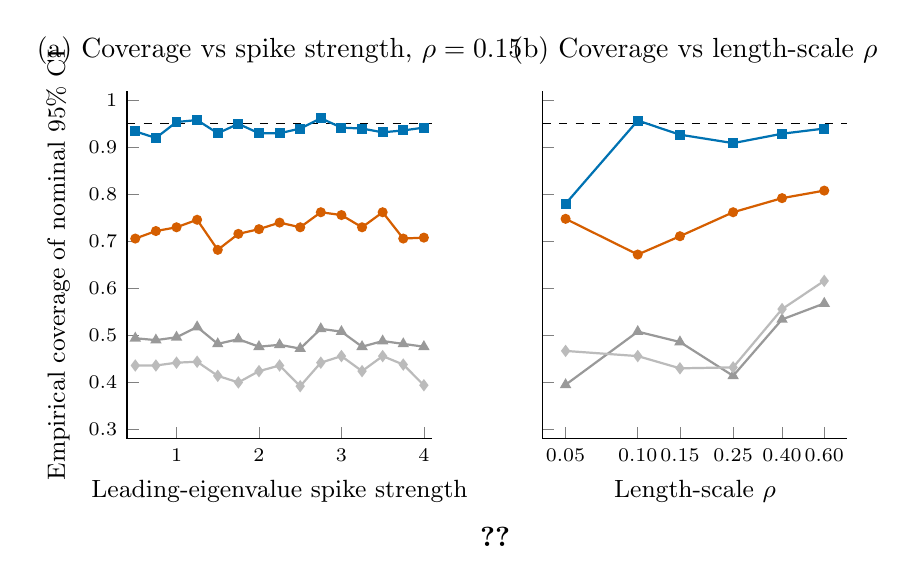
\begin{tikzpicture}
\begin{axis}[
    causalre body, name=dkA,
    xlabel={Leading-eigenvalue spike strength},
    ylabel={Empirical coverage of nominal $95\%$ CI},
    title={(a) Coverage vs spike strength, $\rho = 0.15$},
    xmin=0.4, xmax=4.1, ymin=0.28, ymax=1.02,
    ytick={0.3,0.4,0.5,0.6,0.7,0.8,0.9,1.0},
    legend to name=dkleg,
    legend columns=4,
    legend style={font=\scriptsize, draw=none, fill=none,
                  /tikz/every even column/.append style={column sep=12pt}},
    legend cell align=left,
]
\addplot[black, dashed, thin, forget plot] coordinates {(0.4,0.95) (4.1,0.95)};
\addplot[color=cNYC, thick, mark=square*, mark size=1.4pt] coordinates {
  (0.50,0.934) (0.75,0.920) (1.00,0.954) (1.25,0.958) (1.50,0.930)
  (1.75,0.950) (2.00,0.930) (2.25,0.930) (2.50,0.940) (2.75,0.962)
  (3.00,0.942) (3.25,0.940) (3.50,0.932) (3.75,0.936) (4.00,0.942)
};
\addlegendentry{fixed-$b$, $b = 0.5$, $t_1$}
\addplot[color=cSF, thick, mark=*, mark size=1.4pt] coordinates {
  (0.50,0.706) (0.75,0.722) (1.00,0.730) (1.25,0.746) (1.50,0.682)
  (1.75,0.716) (2.00,0.726) (2.25,0.740) (2.50,0.730) (2.75,0.762)
  (3.00,0.756) (3.25,0.730) (3.50,0.762) (3.75,0.706) (4.00,0.708)
};
\addlegendentry{IM self-normalised $t_{K - 1}$}
\addplot[color=cBOS, thick, mark=triangle*, mark size=1.6pt] coordinates {
  (0.50,0.494) (0.75,0.490) (1.00,0.496) (1.25,0.518) (1.50,0.482)
  (1.75,0.492) (2.00,0.476) (2.25,0.480) (2.50,0.472) (2.75,0.514)
  (3.00,0.508) (3.25,0.476) (3.50,0.488) (3.75,0.482) (4.00,0.476)
};
\addlegendentry{SWM jackknife, $z = 1.96$}
\addplot[color=cMUTE, thick, mark=diamond*, mark size=1.6pt] coordinates {
  (0.50,0.436) (0.75,0.436) (1.00,0.442) (1.25,0.444) (1.50,0.414)
  (1.75,0.400) (2.00,0.424) (2.25,0.436) (2.50,0.392) (2.75,0.442)
  (3.00,0.456) (3.25,0.424) (3.50,0.456) (3.75,0.438) (4.00,0.394)
};
\addlegendentry{Classical, $z = 1.96$}
\end{axis}
\begin{semilogxaxis}[
    causalre body,
    at={(dkA.east)}, anchor=west, xshift=1.4cm,
    xlabel={Length-scale $\rho$}, ylabel={},
    title={(b) Coverage vs length-scale $\rho$},
    xmin=0.04, xmax=0.75, ymin=0.28, ymax=1.02,
    log basis x=10,
    xtick={0.05,0.10,0.15,0.25,0.40,0.60},
    xticklabels={0.05,0.10,0.15,0.25,0.40,0.60},
    ytick={0.3,0.4,0.5,0.6,0.7,0.8,0.9,1.0},
    yticklabels={,,,,,,,},
]
\addplot[black, dashed, thin, forget plot] coordinates {(0.04,0.95) (0.75,0.95)};
\addplot[color=cNYC, thick, mark=square*, mark size=1.4pt, forget plot] coordinates {
  (0.05,0.780) (0.10,0.957) (0.15,0.927) (0.25,0.909) (0.40,0.929) (0.60,0.940)
};
\addplot[color=cSF, thick, mark=*, mark size=1.4pt, forget plot] coordinates {
  (0.05,0.748) (0.10,0.672) (0.15,0.711) (0.25,0.762) (0.40,0.792) (0.60,0.808)
};
\addplot[color=cBOS, thick, mark=triangle*, mark size=1.6pt, forget plot] coordinates {
  (0.05,0.395) (0.10,0.508) (0.15,0.486) (0.25,0.414) (0.40,0.534) (0.60,0.568)
};
\addplot[color=cMUTE, thick, mark=diamond*, mark size=1.6pt, forget plot] coordinates {
  (0.05,0.467) (0.10,0.456) (0.15,0.430) (0.25,0.432) (0.40,0.556) (0.60,0.616)
};
\end{semilogxaxis}
\node[anchor=north] at ($(dkA.south east)+(0.8cm,-1.0cm)$) {\ref{dkleg}};
\end{tikzpicture}
\caption{Empirical coverage of nominal $95\%$ confidence intervals across the Davis--Kahan stress simulation, with $1{,}000$ Monte Carlo replications per cell. The horizontal dashed line in each panel marks the nominal level. Panel (a) varies the leading-eigenvalue spike strength while holding the spatial length-scale at $\rho = 0.15$, and panel (b) varies the length-scale on a log axis while holding the spike strength at its central value. The Salerno--Wu--McCormick jackknife paired with the conventional $z = 1.96$ critical value sits near $0.49$ across both axes, the Ibragimov--M\"uller self-normalised $t_{K - 1}$ paired with the same fold-mean variance sits near $0.73$, and the fixed-$b$ envelope of \citet{sun2008optimal} at $b = 0.5$ reaches roughly $0.93$ at the cost of substantially wider intervals. The seven remaining inference rules reported in Table~\ref{tab:dk_coverage} bunch within the band traced by classical and SWM-with-$z$ and are omitted from the figure for legibility.}
\label{fig:dk_coverage}
\end{figure}
\FloatBarrier

Three readings of Table~\ref{tab:dk_coverage} guide our choice of inference rule for the headline estimate. The first reading is that the Ibragimov--M\"uller construction recovers a substantial coverage improvement over the Salerno--Wu--McCormick jackknife paired with the asymptotic-$z$ critical value, while requiring no bandwidth choice and no kernel specification. Mean coverage moves from $0.48$ to $0.75$ across the $\rho$ sweep, so the construction earns the headline slot for the per-city tables in the main text. The second reading is that the $V_{\text{off}} + V_{\text{between}}$ decomposition of \citet{salerno2026spatially} is mathematically the right correction to the kernel-smoothed Conley HAC, but at $K = 5$ folds the two terms cancel in roughly three-quarters of replications and the net standard-error inflation closes only about three percent of the coverage gap. The third reading is that the fixed-$b$ construction of \citet{sun2008optimal} and \citet{kiefer2005new} at $b = 0.5$ with the $t_1$ critical value reaches mean coverage of $0.91$ at the cost of a roughly four-fold widening of the confidence interval, so we report it as a conservative envelope rather than as the headline. Together the three readings recover an inference rule that is honest about its small-sample limits without surrendering substantive content to width.

The decomposition of the Salerno jackknife variance into its $V_{\text{off}}$ and $V_{\text{between}}$ components clarifies why the $z = 1.96$ pairing under-covers. Empirical fold-mean standard deviation is roughly $3.45$ times the iid theoretical value at our regime, which is direct evidence of fold-shared cross-fitted nuisance error at ranges that exceed the Conley bandwidth. The within-fold kernel-smoothed term $V_{\text{off}}$ and the between-fold variance term $V_{\text{between}}$ are individually large and have opposite signs in a majority of replications, so the additive variance estimator $V_{\text{JK}} = V_{\text{off}} + V_{\text{between}}$ that \citet{salerno2026spatially} prescribe is correctly specified but provides only a small inflation of the realised standard error. The remedy under fixed-$K$ asymptotics is to widen the critical value rather than to enlarge the variance estimator, which is exactly what the Ibragimov--M\"uller and fixed-$b$ constructions do.

\end{document}